\documentclass[a4paper, 10pt]{scrartcl}\usepackage[]{graphicx}\usepackage[]{xcolor}
% maxwidth is the original width if it is less than linewidth
% otherwise use linewidth (to make sure the graphics do not exceed the margin)
\makeatletter
\def\maxwidth{ %
  \ifdim\Gin@nat@width>\linewidth
    \linewidth
  \else
    \Gin@nat@width
  \fi
}
\makeatother

\definecolor{fgcolor}{rgb}{0.345, 0.345, 0.345}
\newcommand{\hlnum}[1]{\textcolor[rgb]{0.686,0.059,0.569}{#1}}%
\newcommand{\hlstr}[1]{\textcolor[rgb]{0.192,0.494,0.8}{#1}}%
\newcommand{\hlcom}[1]{\textcolor[rgb]{0.678,0.584,0.686}{\textit{#1}}}%
\newcommand{\hlopt}[1]{\textcolor[rgb]{0,0,0}{#1}}%
\newcommand{\hlstd}[1]{\textcolor[rgb]{0.345,0.345,0.345}{#1}}%
\newcommand{\hlkwa}[1]{\textcolor[rgb]{0.161,0.373,0.58}{\textbf{#1}}}%
\newcommand{\hlkwb}[1]{\textcolor[rgb]{0.69,0.353,0.396}{#1}}%
\newcommand{\hlkwc}[1]{\textcolor[rgb]{0.333,0.667,0.333}{#1}}%
\newcommand{\hlkwd}[1]{\textcolor[rgb]{0.737,0.353,0.396}{\textbf{#1}}}%
\let\hlipl\hlkwb

\usepackage{framed}
\makeatletter
\newenvironment{kframe}{%
 \def\at@end@of@kframe{}%
 \ifinner\ifhmode%
  \def\at@end@of@kframe{\end{minipage}}%
  \begin{minipage}{\columnwidth}%
 \fi\fi%
 \def\FrameCommand##1{\hskip\@totalleftmargin \hskip-\fboxsep
 \colorbox{shadecolor}{##1}\hskip-\fboxsep
     % There is no \\@totalrightmargin, so:
     \hskip-\linewidth \hskip-\@totalleftmargin \hskip\columnwidth}%
 \MakeFramed {\advance\hsize-\width
   \@totalleftmargin\z@ \linewidth\hsize
   \@setminipage}}%
 {\par\unskip\endMakeFramed%
 \at@end@of@kframe}
\makeatother

\definecolor{shadecolor}{rgb}{.97, .97, .97}
\definecolor{messagecolor}{rgb}{0, 0, 0}
\definecolor{warningcolor}{rgb}{1, 0, 1}
\definecolor{errorcolor}{rgb}{1, 0, 0}
\newenvironment{knitrout}{}{} % an empty environment to be redefined in TeX

\usepackage{alltt}
\usepackage[ngerman]{babel}
% -----------------------------------------------------------------------

% -----------------------------------------------------------------------
%% ------------------------------------------------------------
%% by J.Kruppa on Friday, February 11, 2022 (11:31)
%% \def\mainDir{\Sexpr{exam_path}}
\def\source{/Users/jokruppa/source/tex}
\usepackage[margin=2cm, includefoot]{geometry}
\setlength{\parindent}{0cm}
\usepackage{booktabs}
\usepackage{amsmath}
\usepackage{scalerel,amssymb}
\usepackage{setspace}
\def\csquare{{\Large $\boxtimes$}}
\def\msquare{{\Large $\square$}}
\usepackage[normalem]{ulem}
\usepackage{array}
\usepackage{xcolor}
\usepackage{float}
\usepackage{currfile}
\usepackage{tikz}
\usepackage[nomessages]{fp}

%% beamer defs
\def\lecture{Klausurfragen der Bio Data Science}

%% exam defs
\def\examtitle{\lecture}
\def\exammodule{
\vspace{-1.75cm}  
\begin{graybox}{}
\vspace{2Ex}
\textbf{\large Name:} \rule[0ex]{16.75em}{.4pt}
\hfill \textnormal{\textit{Nicht bestanden:}} \msquare \\[2.5Ex]
\textbf{\large Vorname:} \rule[0ex]{15em}{.4pt} \\[2.5Ex]
\textbf{\large Matrikelnummer:} \rule[0ex]{10.8em}{.4pt}
\hfill Endnote: \rule[0ex]{7em}{.4pt} 
\end{graybox}
\vspace{3Ex}
\phantom{text}
}
\def\examsemester{Sommersemester \& Wintersemester}
\def\examdate{\today}
%% ------------------------------------------------------------
\definecolor{darkblue}{rgb}{0,0,.5}
\definecolor{darkpurple}{rgb}{0.4117, 0.2, 0.4117}
\definecolor{uni}{rgb}{0,0.3137,0.6078}
\definecolor{gray}{gray}{0.7}

\usepackage{tcolorbox}
\definecolor{logo1}{RGB}{0, 158, 227}
\definecolor{gray5}{RGB}{247, 247, 247}
\definecolor{gray2}{RGB}{102, 102, 102}

\newtcolorbox{graybox}[1]{
  colback=gray5,%%red!5!white,
  colframe=gray2,%%red!75!black,
  fonttitle=\bfseries\Large,
  %%valign=center,
  fontupper=\large,
  before skip=10pt plus 2pt,
  after skip=20pt plus 4pt,
  title=#1}

\newtcolorbox{takehomebox}[1]{
  colback=gray5,%%red!5!white,
  colframe=logo1,%%red!75!black,
  fonttitle=\bfseries\Large,
  %%valign=center,
  fontupper=\large,
  before skip=10pt plus 2pt,
  after skip=10pt plus 2pt,
  title=#1}

\def\Rlogo{
\includegraphics[width = 0.5cm]{\string~/Documents/GitHub/exam/img/Rlogo}\;}

\usepackage[scaled=.90]{helvet} 
\usepackage{fancyhdr}
\usepackage{lastpage}
\usepackage{hyperref}
\hypersetup{
    colorlinks=true,       % false: boxed links; true: colored links
    linkcolor=black,          % color of internal links 
    urlcolor=magenta           % color of external links
}
\renewcommand{\familydefault}{\sfdefault}

\title{
\large \exammodule \\[5Ex]
\Huge \examtitle \\[2Ex] 
\Large Hochschule Osnabr{\"u}ck
}
\author{Pr{\"u}fer: Prof. Dr. Jochen Kruppa \\
Fakult{\"a}t f{\"u}r Agrarwissenschaften und Landschaftsarchitektur \\ 
j.kruppa@hs-osnabrueck.de}
\date{Version vom \examdate}

%% ------------------------------------------------------------
%% by J.Kruppa on Tuesday, September 23, 2014 (12:50)
%% Header
\renewcommand{\headrulewidth}{0pt}
\renewcommand{\footrulewidth}{0pt}
\pagestyle{fancy}

\fancyhf{}
\fancyhead[L]{}
\fancyhead[R]{}
\fancyfoot[R]{\thepage}
\fancyfoot[L]{\footnotesize \examtitle}

\fancypagestyle{empty}{
 \fancyhf{}
 \fancyhead[L]{}
 \fancyhead[R]{}
 \fancyfoot[R]{\thepage}
 \fancyfoot[L]{\footnotesize \examtitle}
}

\usepackage{arevtext,arevmath}

\newcommand\Tstrut{\rule{0pt}{2.6ex}}         % = `top' strut
\newcommand\Bstrut{\rule[-0.9ex]{0pt}{0pt}}   % = `bottom' strut
\def\strut{\Tstrut\Bstrut}

\def\textpoints{60}
\FPeval{\overallpoints}{clip(\textpoints + 20)}
% -----------------------------------------------------------------------

% -----------------------------------------------------------------------
\IfFileExists{upquote.sty}{\usepackage{upquote}}{}
\begin{document}
% -----------------------------------------------------------------------

\begin{graybox}{Checkbox für die Version vom \today}
  \Large Die gesamte Klausur beinhaltet aktuell in Summe
  \textbf{126}
  Fragen.\\[1Ex]
  Davon sind \textbf{50} Multiple
  Choice Fragen sowie \textbf{76} Rechen- und
  Textaufgaben.
\end{graybox}

\vfill

\begin{takehomebox}{Frequently asked questions (FAQ)}
  \paragraph{Was ist das hier?} Im Folgenden findet sich die Sammlung
  \textit{aller} Klausurfragen der Bio Data Science über \textit{alle}
  Veranstaltungen, die ich an der Fakultät für Agrarwissenschaften und
  Landschaftsarchitektur anbiete.
  \vspace{1Ex}
  \paragraph{Sind aber ein bisschen \textit{viele} Fragen...} Ja, das
  stimmt. Die Überlegung welche Fragen zur Veranstaltung
  passen obliegt dem Studierenden. Gerne stehe ich für Rückfragen
  bereit. Teilweise sind Fragen auch ähnlich.
  \vspace{1Ex}
  \paragraph{Sind die Fragen fix?} Ein klares Jein. Die Zahlen und die
  \textit{Reihenfolge} der Aufgaben - auch im Multiple Choice Teil - werden
  sich ändern, da die Klausurfragen zufällig erstellt werden. Die
  Aufgaben\textit{fragen} hindoch werden die gleichen Fragen bleiben.
  \vspace{1Ex}
  \paragraph{Okay, aber woher weiß ich jetzt welche Fragen zu meiner
    Veranstaltung gehören?} Das ist der Trick. Durch das Durchlesen und das
  selbstständige Sortieren der Fragen merkt man
  ziemlich schnell, welche Inhalte zu der Veranstaltung gehören und welche
  nicht. Ist also alles Teil des Lernprozesses. \textit{Und} wenn
  Unsicherheiten da sind, gerne in der Wiederholungsveranstaltung - letzte
  Vorlesung - einfach mich fragen.
  \vspace{1Ex}
  \paragraph{Wie sieht denn die finale Klausur aus?} Die Klausur hat am
  Ende 10 Multiple Choice Fragen mit jeweils 2 Punkten sowie Rechen- und
  Textaufgaben mit in Summe ca. 60 Punkten. Ich peile daher eine Klausur
  mit 80 Punkten an, wobei 40 Punkte zum Bestehen der Klausur notwendig
  sind. \textcolor{red}{Bei geteilten Veranstaltungen
    mit mehr als einem Dozenten ändert sich die Zusammensetzung der
    endgültigen Punkteanzahl!}
  \vspace{1Ex}
  \paragraph{Sind aber mehr als \textit{zehn} Multiple Choice Fragen...} Ja,
  aber es werden in der finalen Klausur nur zehn Multiple Choice Fragen
  sein. Ich wähle die Fragen dann zufällig aus. Ich berücksichtige
  natürlich die Veranstaltung und das Lernniveau.
  \vspace{1Ex}
  \paragraph{Solange kann ich nicht warten...} Dann einfach eine Mail an
  mich schreiben:
  \begin{center}
    \url{j.kruppa@hs-onsabrueck.de}
  \end{center}
  Ich versuche dann die Frage kurzfristig zu beantworten oder
  aber in der Vorlesung nochmal (anonym) aufzugreifen.
\end{takehomebox}
  
% -----------------------------------------------------------------------
\maketitle
\thispagestyle{empty}
\clearpage
% -----------------------------------------------------------------------

\begin{graybox}{Erlaubte Hilfsmittel für die Klausur}
  \vspace{1Ex}
  \begin{itemize}
  \item Normaler Taschenrechner ohne Möglichkeit der Kommunikation mit anderen
    Geräten - also ausdrücklich kein Handy!
  \item Eine DIN A4-Seite als beidseitig, selbstgeschriebene,
    handschriftliche Formelsammlung - keine digitalen Ausdrucke. 
  \end{itemize}
\end{graybox}
\vfill

\begin{graybox}{Ergebnis der Klausur}
  \vspace{1Ex}
  \begin{itemize}
  \item[] \rule[0ex]{3em}{.4pt}\, von 20\, Punkten sind aus dem Multiple
    Choice Teil erreicht.
  \item[] \rule[0ex]{3em}{.4pt}\, von \textpoints\, Punkten sind aus dem Rechen- und
    Textteil erreicht. 
  \item[] \rule[0ex]{3em}{.4pt}\, von \overallpoints\, Punkten in Summe.
  \item[] Es wird folgender Notenschlüssel angewendet.   
  \end{itemize}
  \vspace{1ex}
\begin{center}
  \begin{tabular}[c]{cc}
    \toprule
    \textbf{Punkte}	&	\textbf{Note}	\\
    \midrule
    78 - \overallpoints	&	1,0	\\
    75 - 77	&	1,3	\\
    70 - 74	&	1,7	\\
    65 - 69	&	2,0	\\
    59 - 64	&	2,3	\\
    54 - 58	&	2,7	\\
    49 - 53	&	3,0	\\
    44 - 48	&	3,3	\\
    41 - 43	&	3,7	\\
    40	&	4,0	\\
    \bottomrule
  \end{tabular}
\end{center}
  \vspace{1ex}
\begin{itemize}
\item[] Es ergibt sich eine Endnote von \rule[0ex]{4em}{.4pt}.
\end{itemize}
  \vspace{1Ex}
\end{graybox}

% -----------------------------------------------------------------------
\newpage
% -----------------------------------------------------------------------

\begin{graybox}{Multiple Choice Aufgaben}
  \begin{itemize}
  \item Pro Multipe Choice Frage ist \emph{genau} eine Antwort richtig.
  \item \textbf{Übertragen Sie Ihre Kreuze in die Tabelle auf
      dieser Seite.}
  \item Es werden nur Antworten berücksichtigt, die in dieser Tabelle
    angekreuzt sind!
  \end{itemize}

\begin{center}
  \large
  \begin{tabular}{|r|c|c|c|c|c||c|}
    \hline
    & \textbf{A} & \textbf{B} & \textbf{C} & \textbf{D} & \textbf{E} & $\boldsymbol{\checkmark}$\strut\\
    \hline
    1 Aufgabe &   &   &   &   &   & \strut\\
    \hline
    2 Aufgabe &   &   &   &   &   & \strut\\
    \hline
    3 Aufgabe &   &   &   &   &   & \strut\\
    \hline
    4 Aufgabe &   &   &   &   &   & \strut\\
    \hline
    5 Aufgabe &   &   &   &   &   & \strut\\
    \hline
    6 Aufgabe &   &   &   &   &   & \strut\\
    \hline
    7 Aufgabe &   &   &   &   &   & \strut\\
    \hline
    8 Aufgabe &   &   &   &   &   & \strut\\
    \hline
    9 Aufgabe &   &   &   &   &   & \strut\\
    \hline
    10 Aufgabe &   &   &   &   &   & \strut\\
    \hline
  \end{tabular}
\end{center}

\begin{itemize}
\item Es sind \rule[0ex]{2em}{.4pt}\, von 20 Punkten erreicht worden.
\end{itemize}
\end{graybox}

\vfill

\begin{graybox}{Rechen- und Textaufgaben}
  \begin{itemize}
  \item Die Tabelle wird vom Dozenten ausgefüllt.
  \end{itemize}
  \begin{center}
    \large
    \begin{tabular}{|l|c|c|c|c|c|c|c|}
      \hline
      \textbf{Aufgabe} & 11 & 12 & 13 & 14 & 15 & 16 & 17 \strut\\
      \hline
      \textbf{Punkte} & \phantom{1111}  & \phantom{1212}  & \phantom{1313}  & \phantom{1414}  & \phantom{1515}  & \phantom{1616}  & \phantom{1717}
                                                                                                                                    \strut\\
      \hline
  \end{tabular}
\end{center}
\begin{itemize}
\item Es sind \rule[0ex]{2em}{.4pt}\, von \textpoints\, Punkten erreicht worden.
\end{itemize}
\end{graybox}

% -----------------------------------------------------------------------
\clearpage
% -----------------------------------------------------------------------
\begin{graybox}{Multiple Choice Aufgaben}
  \begin{itemize}
  \item Es wird nie mehr als fünfzig Multiple Choice Fragen geben.
  \item Im Laufe der Zeit werden einzelne Fragen durch andere Fragen \textit{ersetzt}, bitte beachten Sie diesen Sachstand, wenn Sie eine \textit{Wiederholungsklausur} im nächsten Semester schreiben. 
  \end{itemize}
\end{graybox}
    

\section{Aufgabe \hfill (2 Punkte)}



Welche Aussage {\"u}ber die \textbf{$confounder$} Adjustierung ist richtig?



\begin{enumerate}
\item [\textbf{A} \msquare] Die $confounder$ ist notwendig um Effekte gegeneinander aufzurechnen. Ohne diese Adjustierung w{"u}rde der eigentliche Effekt nicht richtig gesch{"a}tzt. Daher handelt es sich um eine Adjustierung der Fehlerwahrscheinlichkeiten.
\item [\textbf{B} \msquare] Die $confounder$ Adjustierung wird durchgef{"u}hrt um bei multiplen Vergleichen den Fehler 1. Art zu kontrollieren. Es wird die Irrtumswahrscheinlichkeit adjustiert, daher das $\alpha$-Niveau.
\item [\textbf{C} \msquare] Die $confounder$ Adjustierung wird durchgef{"u}hrt um den Fehler 2. Art zu kontrollieren. Ohne diese Adjustierung w{"u}rde der Fehler 2. Art nicht bei 80\% liegen sondern sehr schnell gegen 0 laufen.
\item [\textbf{D} \msquare] Die $confounder$ Adjustierung wird meist ignoriert. Wenn die Annahmen an den statistischen Test richtig sind, kann auf eine Adjustierung verzichtet werden.
\item [\textbf{E} \msquare] Die $confounder$ Adjustierung wird durchgef{"u}hrt um den Effekt von Interesse, meist die Behandlung, von anderen Effekten zu trennen. Daher eine Adjustierung auf den $\beta$-Werten einer Regression.
\end{enumerate} 

\section{Aufgabe \hfill (2 Punkte)}



Sie haben folgende unadjustierten p-Werte gegeben: 0.42, 0.21, 0.03, 0.02 und 0.34. Sie adjustieren die p-Werte nach
Bonferroni. Welche Aussage ist richtig?



\begin{enumerate}
\item [\textbf{A} \msquare] Nach der Bonferroni-Adjustierung ergeben sich die adjustierten p-Werte von 0.084, 0.042, 0.006, 0.004 und 0.068. Die adjustierten p-Werte werden zu einem $\alpha$-Niveau von 5\% verglichen.
\item [\textbf{B} \msquare] Nach der Bonferroni-Adjustierung ergeben sich die adjustierten p-Werte von 0.084, 0.042, 0.006, 0.004 und 0.068. Die adjustierten p-Werte werden zu einem $\alpha$-Niveau von 1\% verglichen.
\item [\textbf{C} \msquare] Nach der Bonferroni-Adjustierung ergeben sich die adjustierten p-Werte von 1, 1, 0.15, 0.1 und 1. Die adjustierten p-Werte werden zu einem $\alpha$-Niveau von 1\% verglichen.
\item [\textbf{D} \msquare] Nach der Bonferroni-Adjustierung ergeben sich die adjustierten p-Werte von 2.1, 1.05, 0.15, 0.1 und 1.7. Die adjustierten p-Werte werden zu einem $\alpha$-Niveau von 5\% verglichen.
\item [\textbf{E} \msquare] Nach der Bonferroni-Adjustierung ergeben sich die adjustierten p-Werte von 1, 1, 0.15, 0.1 und 1. Die adjustierten p-Werte werden zu einem $\alpha$-Niveau von 5\% verglichen.
\end{enumerate} 

\section{Aufgabe \hfill (2 Punkte)}



Der Datensatz \texttt{PlantGrowth} enth{\"a}lt das Gewicht von Pflanzen, die
unter einer Kontrolle und zwei verschiedenen Behandlungsbedingungen erzielt
wurden. Nach der Berechnung einer einfaktoriellen ANOVA ergibt sich ein
$\eta^2 = 0.29$. Welche Aussage ist richtig?



\begin{enumerate}
\item [\textbf{A} \msquare] Das $\eta^2$ ist die Korrelation der ANOVA. Mit der Ausnahme, dass 0 der beste Wert ist.
\item [\textbf{B} \msquare] Das $\eta^2$ beschreibt den Anteil der Varianz, der von den Behandlungsbedingungen erkl{"a}rt wird. Das $\eta^2$ ist damit mit dem $R^2$ aus der linearen Regression zu vergleichen.
\item [\textbf{C} \msquare] Die Berechnung von $\eta^2$ ist ein Wert f{"u}r die Interaktion.
\item [\textbf{D} \msquare] Das $\eta^2$ beschreibt den Anteil der Varianz, der von den Behandlungsbedingungen nicht erkl{"a}rt wird. Somit der Rest an nicht erkl{"a}rbarer Varianz.
\item [\textbf{E} \msquare] Das $\eta^2$ ist ein Wert f{"u}r die G{"u}te der ANOVA. Je kleiner desto besser. Ein $\eta^2$ von 0 bedeutet ein perfektes Modell mit keiner Abweichung. Die Varianz ist null.
\end{enumerate} 

\section{Aufgabe \hfill (2 Punkte)}

Die folgende Abbildung enth{\"a}lt die Daten aus einer Studie zur
Bewertung der Wirkung von Vitamin C auf das Zahnwachstum bei
Meerschweinchen. Der Versuch wurde an 60 Schweinen durchgef{\"u}hrt, wobei
jedes Tier eine von drei Vitamin-C-Dosen (0.5, 1 und 1.5 mg/Tag) {\"u}ber eine
von zwei Verabreichungsmethoden mit Orangensaft (OJ)  oder
Ascorbins{\"a}ure (VC) erhielt. 



{\centering 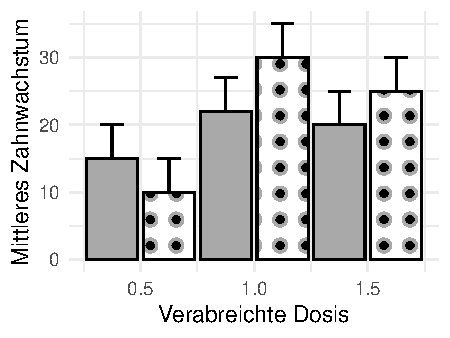
\includegraphics[width=\maxwidth]{img/mc-anova-02-a-1} 

}




Welche Aussage ist richtig im Bezug auf eine zweifaktorielle ANOVA?



\begin{enumerate}
\item [\textbf{A} \msquare] Eine starke Interaktion ist zu erwarten. Die Geraden schneiden sich und die Abst{"a}nde sind nicht gleichbleibend.
\item [\textbf{B} \msquare] Keine Interaktion liegt vor. Die Geraden scheiden sich und laufen nicht parallel.
\item [\textbf{C} \msquare] Eine starke Interaktion liegt vor. Die Geraden laufen parallel und schneiden sich nicht.
\item [\textbf{D} \msquare] Keine Interaktion ist zu erwatzen. Die Geraden der Verabreichungsmethode laufen parallel und mit {"a}hnlichen Abst{"a}nden.
\item [\textbf{E} \msquare] Eine leichte Interaktion ist zu erwarten. Die Geraen schneiden sich noch nicht, aber die Abst{"a}nde unterscheiden sich stark.
\end{enumerate} 

\section{Aufgabe \hfill (2 Punkte)}

Eine einfaktorielle ANOVA berechnet eine Teststatistik um zu die Nullhypothese abzulehnen. Welche Aussage {\"u}ber die Teststatistik der ANOVA ist richtig?



\begin{enumerate}
\item [\textbf{A} \msquare] Die ANOVA berechnet die T-Statistik indem den Mittelwertsunterschied der Gruppen simultan durch die Standardabweichung der Gruppen teilt. Wenn die T-Statistik h{"o}her als 1.96 ist, kann die Nullhypothese abgelehnt werden.
\item [\textbf{B} \msquare] Die ANOVA berechnet die F-Statistik indem die MS der Behandlung durch die MS des Fehlers geteilt werden. Wenn die F-Statistik sich der 0 ann{"a}hert kann die Nullhypothese nicht abgelehnt werden.
\item [\textbf{C} \msquare] Die ANOVA berechnet die T-Statistik aus der Multiplikation der MS Behandlung mit der MS der Fehler. Wenn die F-Statistik genau 0 ist, kann die Nullhypothese abgelehnt werden.
\item [\textbf{D} \msquare] Die ANOVA berechnet die F-Statistik indem die MS des Fehlers durch die MS der Behandlung geteilt werden. Wenn die F-Statistik sich der 1 ann{"a}hert kann die Nullhypothese nicht abgelehnt werden.
\item [\textbf{E} \msquare] Die ANOVA berechnt die F-Statistik aus den SS Behandlung geteilt durch die SS Fehler.
\end{enumerate} 

\section{Aufgabe \hfill (2 Punkte)}




Sie haben das abstrakte Modell $Y \sim X$ mit $X$ als Faktor mit zwei
Leveln vorliegen. Welche Aussage {\"u}ber $s^2_1 \neq s^2_2$ ist richtig?



\begin{enumerate}
\item [\textbf{A} \msquare] Es liegt Varianzhetrogenit{"a}t vor.
\item [\textbf{B} \msquare] Es handelt sich um ein unbalanciertes Design
\item [\textbf{C} \msquare] Es liegt Varianzhomogenit{"a}t vor.
\item [\textbf{D} \msquare] Es handelt sich um abh{"a}ngige Beobachtungen.
\item [\textbf{E} \msquare] Es handelt sich um ein balanciertes Design.
\end{enumerate} 

\section{Aufgabe \hfill (2 Punkte)}

Die Mindestanzahl an Beobachtungen f{\"u}r eine Zelle der Vierfeldertafel bei
der Nutzung eines Chi-Quadrat-Testes ist...



\begin{enumerate}
\item [\textbf{A} \msquare] 10 Beobachtungen
\item [\textbf{B} \msquare] 2 Beobachtungen
\item [\textbf{C} \msquare] 5 Beobachtungen
\item [\textbf{D} \msquare] 1 Beobachtung
\item [\textbf{E} \msquare] 0 Beobachtungen
\end{enumerate} 

\section{Aufgabe \hfill (2 Punkte)}




Welche Aussage {\"u}ber den Korrelationskoeffizienten nach Spearman
ist richtig?



\begin{enumerate}
\item [\textbf{A} \msquare] Der Korrelationskoeffizienten nach Spearman wird genutzt, wenn das Outcome Y normalverteilt ist. Der Korrelationskoeffizienten liegt zwischen 0 und 1.
\item [\textbf{B} \msquare] Der Korrelationskoeffizienten nach Spearman wird genutzt, wenn der Korrelationskoeffizienten zwischen -1 und 1 liegt. Dann sind die Residuen normalverteilt.
\item [\textbf{C} \msquare] Der Korrelationskoeffizienten nach Spearman wird genutzt, wenn das Outcome Y normalverteilt ist. Der Korrelationskoeffizienten liegt zwischen -1 und 1.
\item [\textbf{D} \msquare] Der Korrelationskoeffizienten nach Spearman wird genutzt, wenn das Outcome Y nicht normalverteilt ist. Der Korrelationskoeffizienten liegt zwischen 0 und 1.
\item [\textbf{E} \msquare] Der Korrelationskoeffizienten nach Spearman wird genutzt, wenn das Outcome Y nicht normalverteilt ist. Der Korrelationskoeffizienten liegt zwischen -1 und 1.
\end{enumerate} 

\section{Aufgabe \hfill (2 Punkte)}




Berechnen Sie den Mittelwert und Standardabweichung von $y$ mit 10, 16, 9, 9 und 9.



\begin{enumerate}
\item [\textbf{A} \msquare] Es ergibt sich 11.6 +/- 1.525
\item [\textbf{B} \msquare] Es ergibt sich 10.6 +/- 9.3
\item [\textbf{C} \msquare] Es ergibt sich 10.6 +/- 3.05
\item [\textbf{D} \msquare] Es ergibt sich 10.6 +/- 1.525
\item [\textbf{E} \msquare] Es ergibt sich 9.6 +/- 4.65
\end{enumerate} 

\section{Aufgabe \hfill (2 Punkte)}




Berechnen Sie den Median, das $1^{st}$ Quartile sowie das $3^{rd}$ Quartile von $y$ mit 21, 26, 9, 23, 34, 33 und 51.



\begin{enumerate}
\item [\textbf{A} \msquare] Es ergibt sich 26 [21, 34]
\item [\textbf{B} \msquare] Es ergibt sich 26 +/- 34
\item [\textbf{C} \msquare] Es ergibt sich 26 +/- 21
\item [\textbf{D} \msquare] Es ergibt sich 28 [22, 35]
\item [\textbf{E} \msquare] Es ergibt sich 28 +/- 21
\end{enumerate}

\section{Aufgabe \hfill (2 Punkte)}

Eine der g{\"a}ngigsten Methode der Statistik um einen Fehler zu bestimmen ist...



\begin{enumerate}
\item [\textbf{A} \msquare] ... die Methode der aufaddierten, quadrierten Abst{"a}nde.
\item [\textbf{B} \msquare] ... die Methode des absoluten Abstands.
\item [\textbf{C} \msquare] ... die Methode des absoluten, quadrierten Abstands.
\item [\textbf{D} \msquare] ... die Methode der aufaddierten, absoluten Abst{"a}nde.
\item [\textbf{E} \msquare] ... das Produkt der kleinsten Quadrate.
\end{enumerate} 

\section{Aufgabe \hfill (2 Punkte)}

Welche Aussage {\"u}ber Cook's d und Cohen's d ist richtig? 



\begin{enumerate}
\item [\textbf{A} \msquare] Wir nutzen Cook's d um Outlier in den Daten zu finden und Cohen's d um einen standardisierten Effektsch{"a}tzer f{"u}r Gruppenvergeliche zu erhalten.
\item [\textbf{B} \msquare] Wir nutzen Cook's d um Outlier in den Daten zu finden und Cohen's d um standardisierte Outlier f{"u}r Gruppenvergeliche zu erhalten.
\item [\textbf{C} \msquare] Wir nutzen Cook's d um Outlier in den Daten zu finden. Cohen's d findet auch Outlier, ist aber ein veraltetetes Konzept in der Statistik.
\item [\textbf{D} \msquare] Wir nutzen Cohen's d um Outlier in den Daten zu finden und Cook's d um einen standardisierten Effektsch{"a}tzer f{"u}r Gruppenvergeliche zu erhalten.
\item [\textbf{E} \msquare] Wir nutzen Cook's d um Outlier in den Daten zu finden und Cohen's d um einen nicht standardisierten Effektsch{"a}tzer f{"u}r Gruppenvergeliche zu erhalten.
\end{enumerate} 

\section{Aufgabe \hfill (2 Punkte)}



Die empfohlene Mindestanzahl an Beobachtungen f{\"u}r einen Dotplot sind...



\begin{enumerate}
\item [\textbf{A} \msquare] 10 Beobachtungen.
\item [\textbf{B} \msquare] mindestens 20 Beobachtungen.
\item [\textbf{C} \msquare] 5 und mehr Beobachtungen.
\item [\textbf{D} \msquare] 1 Beobachtung.
\item [\textbf{E} \msquare] 2-5 Beobachtungen.
\end{enumerate} 

\section{Aufgabe \hfill (2 Punkte)}



Mit einem Boxplot wird Folgendes in der Statistik und der explorativen Datenanalyse haupts{\"a}chlich dargestellt.



\begin{enumerate}
\item [\textbf{A} \msquare] Die Eigenschaften von Daten anhand der fehlenden Werte und den Leveln eines Faktors $x$.
\item [\textbf{B} \msquare] Die Verteilung von Daten. Meistens dem Outcome oder auch $y$ genannt. Die Darstellung ist auch mit einer kleinen Fallzahl von Minimum 5 Beoabchtungen m{"o}glich.
\item [\textbf{C} \msquare] Die Verteilung von Daten. Auch 2 bis 5 Beonachtungen k{"o}nnen noch dargestellt werden.
\item [\textbf{D} \msquare] Die Eigenschaften von Daten aufgeteilt nach zwei Gruppen eines Faktors $x$.
\item [\textbf{E} \msquare] Die Verteilung von Daten. Meistens dem Outcome oder auch $y$ genannt. Hierbei ist eine hohe Fallzahl notwendig mit mehr als 20 Beoabchtungen.
\end{enumerate} 

\section{Aufgabe \hfill (2 Punkte)}



Nachdem Sie in einem Experiment die Daten $D$ erhoben haben, berechnen Sie den
Mittelwert und den Median. Der Mittelwert $\bar{y}$ und der Median
$\tilde{y}$ unterscheiden sich. Welche Aussage ist richtig?




\begin{enumerate}
\item [\textbf{A} \msquare] Da sich der Mittelwert und der Median nicht unterscheiden, liegen vermutlich Outlier in den Daten vor.
\item [\textbf{B} \msquare] Da sich der Mittelwert und der Median unterscheiden, liegen vermutlich keine Outlier in den Daten vor.
\item [\textbf{C} \msquare] Da sich der Mittelwert und der Median unterscheiden, liegen vermutlich Outlier in den Daten vor. Wir untersuchen den Datensatz nach auff{"a}lligen Beobachtungen.
\item [\textbf{D} \msquare] Da sich der Mittelwert und der Median unterscheiden, ist der Datensatz nicht zu verwenden. Mittelwert und Median m{"u}ssen gleich sein.
\item [\textbf{E} \msquare] Da sich der Mittelwert und der Median nicht unterscheiden, liegen vermutlich keine Outlier in den Daten vor. Wir verweden den Datensatz so wie er ist.
\end{enumerate}

\section{Aufgabe \hfill (2 Punkte)}

Price et al. (2016) untersuchte die Auswirkungen des Bergbaus und der
Talauff{\"u}llung auf den Bestand und die H{\"a}ufigkeit von Bachsalamandern. Um
den Effekt zu Berechnen nutze Price et al. (2016) eine Possion-Regression
auf die Anzahl an aufgefundenen Bachsalamandern an den jeweiligen
Suchorten. Welche Aussage zur Possion-Regression auf Z{\"a}hldaten ist richtig?






\begin{enumerate}
\item [\textbf{A} \msquare] Die Possion-Regression sch{"a}tzt nur einen Verteilungsparameter. Deshalb muss {"u}berpr{"u}ft werden, ob Overdispersion vorliegt. Mit einer gesch{"a}tzen Overdispersion von 2.63 liegt Overdispersion vor. Damit kann keine Possion-Regression gerechnet werden. Die L{"o}sung ist eine Gaussian Regression mit Nullanpassung.
\item [\textbf{B} \msquare] Die Possion-Regression sch{"a}tzt drei Verteilungsparameter. Deshalb muss {"u}berpr{"u}ft werden, ob Overdispersion vorliegt. Mit einer gesch{"a}tzen Overdispersion von 2.63 liegt Overdispersion vor. Die L{"o}sung ist die Nutzung von nur zwei der drei Verteilungsparameter: $\gamma_1$ und $\gamma_3$.
\item [\textbf{C} \msquare] Die Possion-Regression sch{"a}tzt nur einen Verteilungsparameter. Deshalb muss {"u}berpr{"u}ft werden, ob Overdispersion vorliegt. Mit einer gesch{"a}tzen Overdispersion von 2.63 liegt keine Overdispersion vor. Overdispersion liegt vor, wenn die gesch{"a}tzte Overdispersion unter 1 liegt.
\item [\textbf{D} \msquare] Die Possion-Regression sch{"a}tzt nur einen Verteilungsparameter. Deshalb muss {"u}berpr{"u}ft werden, ob Overdispersion vorliegt. Mit einer gesch{"a}tzen Overdispersion von 2.63 liegt Overdispersion vor. Die L{"o}sung ist die Nutzung einer anderen Verteilungsfamilie wie die Quasipossion Verteilung.
\item [\textbf{E} \msquare] Die Possion-Regression sch{"a}tzt zwei Verteilungsparameter. Deshalb muss {"u}berpr{"u}ft werden, ob Overdispersion vorliegt. Mit einer gesch{"a}tzen Overdispersion von 2.63 liegt keine Overdispersion vor.
\end{enumerate}

\section{Aufgabe \hfill (2 Punkte)}

In dem folgenden Histogramm von $n = 200$ Pflanzen ist welche Verteilung
mit welchen korrekten Verteilungsparametern dargestellt?



{\centering 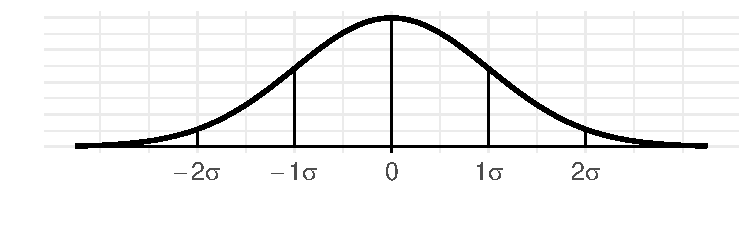
\includegraphics[width=\maxwidth]{img/mc-distribution-02-a-1} 

}







\begin{enumerate}
\item [\textbf{A} \msquare] Es handelt sich um eine Poisson-Verteilung mit Pois(10).
\item [\textbf{B} \msquare] Es handelt sich um eine Normalverteilung mit N(10, 5).
\item [\textbf{C} \msquare] Es handelt sich um eine Binomial-Verteilung mit Binom(10).
\item [\textbf{D} \msquare] Eine Standardnormalverteilung mit N(0,1).
\item [\textbf{E} \msquare] Eine rechtsschiefe, multivariate Normalverteilung.
\end{enumerate}

\section{Aufgabe \hfill (2 Punkte)}




Price et al. (2016) untersuchte die Auswirkungen des Bergbaus und der
Talauff{\"u}llung auf den Bestand und die H{\"a}ufigkeit von Bachsalamandern. Um
den Effekt zu Berechnen nutze Price et al. (2016) eine Possion-Regression
auf die Anzahl an aufgefundenen Bachsalamandern an den jeweiligen
Suchorten. Nach einer statistischen Beratung wurde Ihm nahegelegt auf
Overdispersion zu achten, wenn er statistische Aussagen zur Signifikanz
treffen will. Price et al. (2016) sch{\"a}tzt zwei Modelle. Modell 1 mit einer
Possion Verteilung und Modell 2 mit einer Quasi-Poisson Verteilung. Welche
Aussage zu einer gesch{\"a}tzen Overdispersion von 3.15 ist
richtig?




\begin{enumerate}
\item [\textbf{A} \msquare] Bei einer gesch{"a}tzen Overdispersion h{"o}her als 1.5 ist von keiner Overdispersion in den Daten auszugehen. Dennoch sind die p-Werte zu klein, dass diese p-Werte nat{"u}rlich entstanden sein k{"o}nnten. Die p-Werte m{"u}ssen adjustiert werden.
\item [\textbf{B} \msquare] Bei einer gesch{"a}tzen Overdispersion h{"o}her als 1.5 ist von Overdispersion in den Daten auszugehen. Daher wird die Varianz systematisch untersch{"a}tzt, was zu h{"o}heren p-Werten f{"u}hrt. Daher gibt es weniger signifikante Ergebnisse als es in Wirklichkeit gibt. Daher ist das Modell 1 die bessere Wahl.
\item [\textbf{C} \msquare] Bei einer gesch{"a}tzen Overdispersion h{"o}her als 1.5 ist von Overdispersion in den Daten auszugehen. Daher wird die Varianz systematisch {"u}bersch{"a}tzt, was zu h{"o}heren p-Werten f{"u}hrt. Daher gibt es mehr signifikante Ergebnisse als es in Wirklichkeit gibt. Daher ist das Modell 1 die bessere Wahl
\item [\textbf{D} \msquare] Bei einer gesch{"a}tzen Overdispersion h{"o}her als 1.5 ist von Overdispersion in den Daten auszugehen. Daher wird die Varianz systematisch untersch{"a}tzt, was zu kleineren p-Werten f{"u}hrt. Daher gibt es mehr signifikante Ergebnisse als es in Wirklichkeit gibt. Daher ist das Modell 2 die bessere Wahl.
\item [\textbf{E} \msquare] Das vergleichen von verschiedenen Modellen muss erst {"u}ber ein AIC Kriterium erfolgen. Die Absch{"a}tzung {"u}ber die Overdispersion ist nicht notwendig. Die Varianzen werden sp{"a}ter in einer ANOVA adjustiert. Die Confounder Adjustierung.
\end{enumerate}

\section{Aufgabe \hfill (2 Punkte)}

In einem Zuchtexperiment messen wir die Ferkel verschiedener Sauen. Die
Ferkel einer Muttersau sind daher im statistischen Sinne... 



\begin{enumerate}
\item [\textbf{A} \msquare] Untereinander stark korreliert. Die Ferkel sind von einer Mutter und sommit miteinander korreliert. Dies wird in der Statistik jedoch meist nicht modelliert.
\item [\textbf{B} \msquare] Untereinander unabh{"a}ngig. Sollten die M{"u}tter verwandt sein, so ist die Varianzstruktur {"a}hnlich und muss modelliert werden.
\item [\textbf{C} \msquare] Untereinander abh{"a}ngig, wenn die M{"u}tter ebenfalls miteinander verwandt sind. Erst die Abh{"a}ngigkeit 2. Grades wird in der Statistik modelliert.
\item [\textbf{D} \msquare] Untereinander abh{"a}ngig. Die Ferkel stammen von einem Muttertier und haben vermutliche eine {"a}hnliche Varianzstruktur.
\item [\textbf{E} \msquare] Untereinander unabh{"a}ngig. Die Ferkel sind eigenst{"a}ndig und ben{"o}tigen keine zus{"a}tzliche Behandlung.
\end{enumerate}

\section{Aufgabe \hfill (2 Punkte)}




Sie haben das abstrakte Modell $Y \sim \mathbf{X}$ vorliegen. Welche Aussage {\"u}ber
$\mathbf{X}$ ist richtig?



\begin{enumerate}
\item [\textbf{A} \msquare] $\mathbf{X}$ beinhaltet die Zeilen. Die Zeilen geben die Verteilungsfamilie vor.
\item [\textbf{B} \msquare] $\mathbf{X}$ beinhaltet eine Spalte. Die Spalte gibt die Verteilungsfamilie vor.
\item [\textbf{C} \msquare] $\mathbf{X}$ beinhaltet mehrere Spalten. Die Spalten geben die Verteilungsfamilie vor.
\item [\textbf{D} \msquare] $\mathbf{X}$ beinhaltet eine Spalte. Die Spalte gibt nicht die Verteilungsfamilie vor.
\item [\textbf{E} \msquare] $\mathbf{X}$ beinhaltet mehrere Spalten. Die Spalten enthalten die Behandlung und weitere potenzielle Einflussvariablen
\end{enumerate}

\section{Aufgabe \hfill (2 Punkte)}




Sie haben das Modell $Y \sim X$ vorliegen und wollen nun ein
kausales Modell rechnen. Welche Aussage ist richtig?



\begin{enumerate}
\item [\textbf{A} \msquare] Ein kausales Modell m{"o}chte die Zusammenh{"a}nge von X auf Y modellieren. Hierbei geht es um die Effekte von X auf Y. Man sagt, wenn X um 1 ansteigt {"a}ndert sich Y um einen Betrag $\beta$.
\item [\textbf{B} \msquare] Ein kausales Modell schliesst grunds{"a}tzlich lineare Modell aus. Es muss ein Graph gefunden werden, der alle Punkte beinhaltet. Erst dann kann das $R^2$ berechnet werden.
\item [\textbf{C} \msquare] Ein kausales Modell ben{"o}tigt mindestens eine Fallzahl von {"u}ber 100 Beobachtungen und darf keine fehlenden Werte beinhalten. Die Varianzkomponenten m{"u}ssen homogen sein.
\item [\textbf{D} \msquare] Ein kausales Modell wird auf einem Trainingsdatensatz trainiert und anschliessend {"u}ber eine explorative Datenanalyse validiert. Signifikanzen {"u}ber $\beta_i$ k{"o}nnen hier nicht festgestellt werden.
\item [\textbf{E} \msquare] Ein kausales Modell basiert auf einem Traingsdatensatz und einem Testdatensatz. Auf dem Trainingsdatensatz wird das Modell trainiert und auf dem Testdatensatz validiert.
\end{enumerate}

\section{Aufgabe \hfill (2 Punkte)}



In der folgenden Abbildung ist der Zusammenhang vom Modell zu der linearen
Regression und der ANOVA skizziert.

\begin{center}
  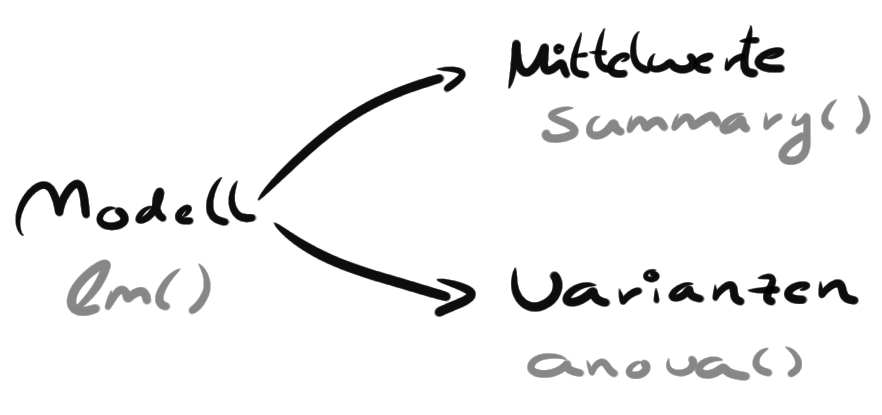
\includegraphics[width = 9cm]{/Users/kruppajo/Documents/GitHub/exam/question/img/mc-modeling-03}
\end{center}

Welche der folgenden Aussagen ist richtig?



\begin{enumerate}
\item [\textbf{A} \msquare] Die Effektsch{"a}tzer aus einem Modell, in diesem Fall ein lineares Modell, erlauben es sowohl eine ANOVA zurechnen sowie auch eine Zusammenfassung der Mittelwerte zu betrachten.
\item [\textbf{B} \msquare] Die Effektsch{"a}tzer aus einem Modell, in diesem Fall ein lineares Modell, erlauben es nur eine ANOVA zurechnen oder eine Zusammenfassung der Mittelwerte zu betrachten. Beides ist nicht m{"o}glich.
\item [\textbf{C} \msquare] Die Effektsch{"a}tzer aus einem Modell, erlauben es nur einen Mittelwertsvergleich zu rechnen.
\item [\textbf{D} \msquare] Die Effektsch{"a}tzer aus einem Modell, erlauben es nur eine ANOVA zu rechnen. 
\item [\textbf{E} \msquare] Die Effektsch{"a}tzer aus einem Modell, in diesem Fall ein polynomes Modell, erlauben es sowohl eine ANOVA zurechnen sowie auch eine Zusammenfassung der Mittelwerte zu betrachten.
\end{enumerate}

\section{Aufgabe \hfill (2 Punkte)}

In der Statistik werden die Daten D modelliert in dem ein Modell der Form
$Y \sim X$ aufgestellt wird. Welche statistische Kenngr{\"o}sse wird modelliert? 



\begin{enumerate}
\item [\textbf{A} \msquare] Die Varianzstruktur wird modelliert.
\item [\textbf{B} \msquare] Die Varianz der X unabh{"a}ngig vom Y wird modelliert.
\item [\textbf{C} \msquare] Die Mittelwerte werden modelliert.
\item [\textbf{D} \msquare] Die Y werden modelliert.
\item [\textbf{E} \msquare] Die X werden modelliert.
\end{enumerate}

\section{Aufgabe \hfill (2 Punkte)}



Sie f{\"u}hren ein Experiment zur Behandlung von Klaueninfektionen bei K{\"u}hen
durch. Bei 3 Tieren finden Sie eine Erkrankung der Klauen vor und
12 Tiere sind gesund. Welche Aussage {\"u}ber den Odds ratio
Effektsch{\"a}tzer ist richtig?



\begin{enumerate}
\item [\textbf{A} \msquare] Es ergibt sich ein Odds ratio von 0.25, da es sich um ein Anteil handelt.
\item [\textbf{B} \msquare] Es ergibt sich ein Odds ratio von 0.2, da es sich um ein Anteil handelt.
\item [\textbf{C} \msquare] Es ergibt sich ein Odds ratio von 4, da es sich um ein Anteil handelt.
\item [\textbf{D} \msquare] Es ergibt sich ein Odds ratio von 0.25, da es sich um eine Chancenverh{"a}ltnis handelt.
\item [\textbf{E} \msquare] Es ergibt sich ein Odds ratio von 0.2, da es sich um eine Chancenverh{"a}ltnis handelt.
\end{enumerate}

\section{Aufgabe \hfill (2 Punkte)}




Welche Aussage {\"u}ber die nicht-parametrische Statistik ist richtig?



\begin{enumerate}
\item [\textbf{A} \msquare] Die nicht-parametrische Statistik basiert auf dem Sch{"a}tzen von Parametern aus einer festgelegten Verteilung. Daher gibt es auch direkt zu interpretierenden Effektsch{"a}tzer.
\item [\textbf{B} \msquare] Die nicht-parametrische Statistik ist ein Vorg{"a}nger der parametrischen Statistik und wurde wegen dem Mangel an Effektsch{"a}tzern nicht mehr ab 1960 genutzt.
\item [\textbf{C} \msquare] Die nicht-parametrische Statistik basiert auf R{"a}ngen. Daher wird jeder Zahl ein Rang zugeteilt. Nur auf den R{"a}ngen wird die Auswertung gerechnet. Daher gibt es auch keinen direkt zu interpretierenden Effektsch{"a}tzer.
\item [\textbf{D} \msquare] Die nicht-parametrische Statistik basiert auf R{"a}ngen. Daher gibt es auch direkt zu interpretierenden Effektsch{"a}tzer.
\item [\textbf{E} \msquare] Die nicht-parametrische Statistik basiert auf dem Sch{"a}tzen von Parametern aus einer a priori festgelegten Verteilung. Daher gibt es auch direkt zu interpretierenden Effektsch{"a}tzer.
\end{enumerate}

\section{Aufgabe \hfill (2 Punkte)}

Die Randomisierung von Beobachtungen bzw. Samples zu den Versuchseinheiten
ist bedeutend in der Versuchsplanung. Welche der folgenden Aussagen ist richtig?



\begin{enumerate}
\item [\textbf{A} \msquare] Randomisierung erlaubt erst die Varianzen zu sch{"a}tzen. Ohne eine Randomisierung ist die Berechnung von Mittelwerten und Varianzen nicht m{"o}glich.
\item [\textbf{B} \msquare] Randomisierung sorgt f{"u}r Strukturgleichheit und erlaubt erst von der Stichprobe auf die Grundgesamtheit zur{"u}ckzuschliessen.
\item [\textbf{C} \msquare] Randomisierung erlaubt erst die Mittelwerte zu sch{"a}tzen. Ohne Randomisierung keine Mittelwerte.
\item [\textbf{D} \msquare] Randomisierung bringt starke Unstrukturiertheit in das Experiment und erlaubt erst von der Stichprobe auf die Grundgesamtheit zur{"u}ckzuschliessen.
\item [\textbf{E} \msquare] Randomisierung war bis 1952 bedeutend, wurde dann aber in Folge besserer Rechnerleistung nicht mehr verwendet. Aktuelle Statistik nutzt keine Randomisierung mehr.
\end{enumerate}

\section{Aufgabe \hfill (2 Punkte)}

Wenn Sie einen Datensatz erstellen, dann ist es ratsam die Spalten und die
Eintr{\"a}ge in englischer Sprache zu verfassen, wenn Sie sp{\"a}ter die Daten in
\Rlogo auswerten wollen. Welcher folgende Grund ist richtig?



\begin{enumerate}
\item [\textbf{A} \msquare] Programmiersprachen k{"o}nnen nur englische Begriffe verarbeiten. Zus{"a}tzliche Pakete k{"o}nnen zwar geladen werden, aber meist funktionieren diese Pakete nicht richtig. Deutsch ist International nicht bedeutend genug.
\item [\textbf{B} \msquare] Alle Funktionen und auch Anwendungen sind in \Rlogo in englischer Sprache. Die Nutzung von deutschen W{"o}rtern ist nicht schick und das ist zu vermeiden.
\item [\textbf{C} \msquare] Die Spracherkennung von \Rlogo ist nicht in der Lage Deutsch zu verstehen.
\item [\textbf{D} \msquare] Es gibt keinen Grund nicht auch deutsche W{"o}rter zu verwenden. Es ist ein Stilmittel.
\item [\textbf{E} \msquare] Im Allgemeinen haben Programmiersprachen Probleme mit Umlauten und Sonderzeichen, die in der deutschen Sprache vorkommen. Eine Nutzung der englischen Sprache umgeht dieses Problem auf einfache Art.
\end{enumerate}

\section{Aufgabe \hfill (2 Punkte)}

Bei der explorativen Datenanalyse (EDA) in \Rlogo gibt es eine richtige Abfolge von Prozessschritten, auch \textit{Circle of life} genannt. Wie lautet die richtige Reihenfolge f{\"u}r die Erstellung einer EDA?



\begin{enumerate}
\item [\textbf{A} \msquare] Wir lesen als erstes die Daten {"u}ber \texttt{read\_excel()} ein, transformieren die Spalten {"u}ber \texttt{mutate()} in die richtige Form und k{"o}nnen dann  {"u}ber \text{ggplot()} uns die Abbildungen erstellen lassen. Wichtig ist, dass wir keine Faktoren sondern nur numerische Variablen vorliegen haben.
\item [\textbf{B} \msquare] Wir lesen die Daten ein und mutieren die Daten. Dabei ist wichtig, dass wir nicht das Paket \texttt{tidyverse} nutzen, da dieses Paket veraltet ist. {"U}ber die Funktion \texttt{library(tidyverse)} entfernen wir das Paket von der Analyse.
\item [\textbf{C} \msquare] Wir transformieren die Spalten {"u}ber \texttt{mutate()} in ein \texttt{tibble} und k{"o}nnen dann {"u}ber \text{ggplot()} uns die Abbildungen erstellen lassen. Dabei beachten wir das wir keine Faktoren in den Daten haben.
\item [\textbf{D} \msquare] Wir lesen die Daten {"u}ber eine generische Funktion \texttt{read()} ein und m{"u}ssen dann die Funktion \texttt{ggplot()} nur noch installieren. Dann haben wir die Abbildungen als \texttt{*.png} vorliegen.
\item [\textbf{E} \msquare] Wir lesen als erstes die Daten {"u}ber \texttt{read\_excel()} ein, transformieren die Spalten {"u}ber \texttt{mutate()} in die richtige Form und k{"o}nnen dann {"u}ber \text{ggplot()} uns die Abbildungen erstellen lassen.
\end{enumerate}

\section{Aufgabe \hfill (2 Punkte)}



In einem Stallexperiment mit $n = 122$ Ferkeln wurden verschiedene
Outcomes gemessen: der Gewichtszuwachs, {\"U}berleben nach 21 Tagen sowie
Anzahl Verletzungen pro 7 Tagen. Zwei Lichtregime wurden als
Einflussfaktor gemessen. Sie erhalten den \Rlogo Output der Funktion
\texttt{tidy()} einer simplen $logistischen$ linearen
Regression. Welche Aussage {\"u}ber den \textbf{Effekt} ist richtig?

\begin{table}[!h]
\centering
\begin{tabular}{ccc}
\toprule
term & estimate & std.error\\
\midrule
(Intercept) & -0.08 & 0.28\\
light\_binhigh & -3.48 & 0.77\\
\bottomrule
\end{tabular}
\end{table}





\begin{enumerate}
\item [\textbf{A} \msquare] In einer logistischen Regression kann kein Effekt roh interpretiert werden. Es muss erst eine Confounderadjustierung durchgef{"u}hrt werden.
\item [\textbf{B} \msquare] In einer logistischen Regression wird die Mittelwertsdifferenz betrachtet. Daher ist der Effekt zwischen den beiden Lichtregimen eine Gewichts{"a}nderung von -3.48
\item [\textbf{C} \msquare] In einer logistischen Regression berechnet man das RR. Daher muss der Sch{"a}tzer des Effektes $\beta_1$ noch exponiert werden. Somit liegt das RR bei 12.08
\item [\textbf{D} \msquare] In einer logistischen Regression muss f{"u}r die Interpretation des Effektes das $\beta_1$ exponiert werden. Somit liegt das OR bei 12.08
\item [\textbf{E} \msquare] Eine logistischen Regression basiert auf dem maximum Likelihood Prinzip. Hierbei kann kein Effekt beschrieben werden. Im Zweifel hilft aber eine Quadrierung der Fehlerqudrate $\epsilon$.
\end{enumerate}

\section{Aufgabe \hfill (2 Punkte)}

In einer linearen Regression werden die $\epsilon$ oder Residuen
gesch{\"a}tzt. Welcher Verteilung folgen die Residuen bei einer optimalen
Modellierung? 



\begin{enumerate}
\item [\textbf{A} \msquare] Die Residuen sind binomialverteilt.
\item [\textbf{B} \msquare] Die Residuen sind normalverteilt mit $\mathcal{N}(0, 1)$.
\item [\textbf{C} \msquare] Die Residuen folgen einer Poissonverteilung mit Pois(0).
\item [\textbf{D} \msquare] Die Residuen sind normalverteilt mit $\mathcal{N}(0, s^2)$.
\item [\textbf{E} \msquare] Die Residuen sind normalverteilt mit $\mathcal{N}(\bar{y}, s^2)$.
\end{enumerate}

\section{Aufgabe \hfill (2 Punkte)}

Welche Aussage {\"u}ber das \textit{generalisierte lineare Modell (GLM)} ist richtig?  



\begin{enumerate}
\item [\textbf{A} \msquare] Das GLM ist eine allgemeine Erweiterung der linearen Regression auf die Normalverteilung.
\item [\textbf{B} \msquare] Das GLM erlaubt auch weitere Verteilungsfamilien f{"u}r das Y bzw. das Outcome in einer linearen Regression zu w{"a}hlen.
\item [\textbf{C} \msquare] Das GLM ist ein faktisch maschineller Lernalgorithmus, der selstst{"a}ndig die Verteilungsfamilie f{"u}r Y w{"a}hlt.
\item [\textbf{D} \msquare] Das GLM ist eine Vereinfachung des LM in R. Mit dem GLM lassen polygonale Regressionen rechnen.
\item [\textbf{E} \msquare] Das GLM erlaubt auch nicht normalverteilte Residuen in der Sch{"a}tzung der Regressionsgrade.
\end{enumerate}

\section{Aufgabe \hfill (2 Punkte)}



Sie rechnen in einer linearen Regression das Modell A und das Modell B. Nun
stellt sich die Frage, welches der beiden Modelle das bessere Modell
ist. Um die Modelle bewerten zu k{\"o}nnen berechnen Sie daf{\"u}r das AIC$_A$ f{\"u}r
Modell A mit 653 und f{\"u}r das Modell B das AIC$_B$ von
287. Welche Aussage {\"u}ber die beiden Modelle ist richtig?



\begin{enumerate}
\item [\textbf{A} \msquare] Da AIC$_A$ < AIC$_B$ ist das Modell A das bessere Modell.
\item [\textbf{B} \msquare] Da AIC$_A$ > AIC$_B$ ist das Modell B das bessere Modell.
\item [\textbf{C} \msquare] Da AIC$_A$ > AIC$_B$ ist das Modell A das bessere Modell.
\item [\textbf{D} \msquare] Da AIC$_A$ < AIC$_B$ ist das Modell B das bessere Modell.
\item [\textbf{E} \msquare] Da AIC$_A$ > 0 ist das Modell A das bessere Modell. Der AIC Wert f{"u}r B wird verworfen.
\end{enumerate}

\section{Aufgabe \hfill (2 Punkte)}

Sie rechnen in eine linearen Regression und erhalten folgenden QQ
Plot. Welche Aussage ist richtig?




{\centering 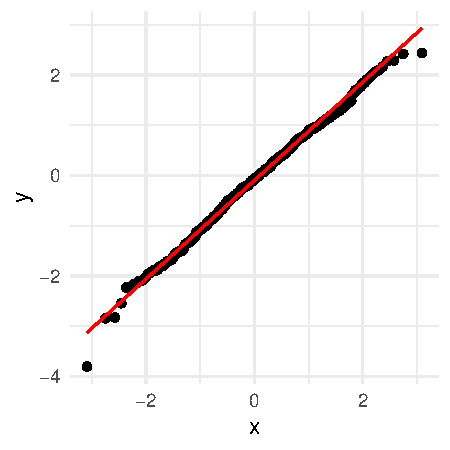
\includegraphics[width=\maxwidth]{img/mc-regression-05-a-1} 

}







\begin{enumerate}
\item [\textbf{A} \msquare] Die Annahme der normalverteilten Residuen ist nicht erf{"u}llt. Die Punkte liegen zum {"u}berwiegenden Teil auf der Geraden.
\item [\textbf{B} \msquare] Die Annahme der normalverteilten Residuen ist nicht erf{"u}llt. Die Punkte liegen zum {"u}berwiegenden Teil nicht auf der Geraden.
\item [\textbf{C} \msquare] Die Annahme der normalverteilten Residuen ist erf{"u}llt. Die Punkte liegen zum {"u}berwiegenden Teil auf der Geraden.
\item [\textbf{D} \msquare] Die Annahme der normalverteilten Residuen ist erf{"u}llt. Die Punkte liegen zum {"u}berwiegenden Teil nicht auf der Geraden.
\item [\textbf{E} \msquare] Die Annahme der normalverteilten Residuen ist erf{"u}llt. Die Punkte liegen zum {"u}berwiegenden Teil nicht auf der Geraden und Korrelation ist negativ.
\end{enumerate}

\section{Aufgabe \hfill (2 Punkte)}

Sie rechnen eine linearen Regression und erhalten folgenden Residual
Plot. Welche Aussage ist richtig?




{\centering 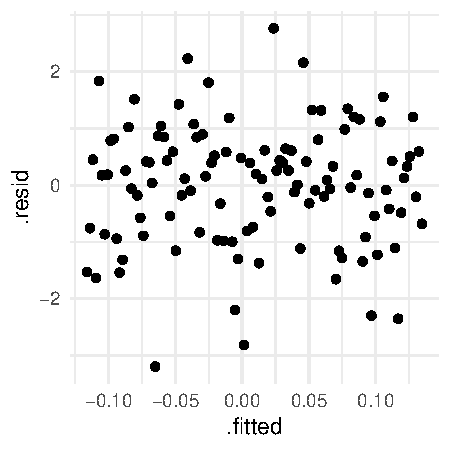
\includegraphics[width=\maxwidth]{img/mc-regression-06-a-1} 

}







\begin{enumerate}
\item [\textbf{A} \msquare] Die Annahme der normalverteilten Residuen ist erf{"u}llt. Es ist ein Muster zu erkennen.
\item [\textbf{B} \msquare] Die Annahme der normalverteilten Residuen ist erf{"u}llt. Die Punkte liegen zum {"u}berwiegenden Teil auf der Diagonalen.
\item [\textbf{C} \msquare] Die Annahme der normalverteilten Residuen ist nicht erf{"u}llt. Vereinzelte Punkte liegen oberhalb bzw. unterhalb der Geraden um die 0 Linie weiter entfernt. Ein klares Muster ist zu erkennen.
\item [\textbf{D} \msquare] Die Annahme der normalverteilten Residuen ist nicht erf{"u}llt. Es ist kein Muster zu erkennen.
\item [\textbf{E} \msquare] Die Annahme der normalverteilten Residuen ist erf{"u}llt. Kein Muster ist zu erkennen und keine Outlier zu beobachten.
\end{enumerate}

\section{Aufgabe \hfill (2 Punkte)}




Sie wollen ein Feldexperiment mit zwei D{\"u}ngestufen durchf{\"u}hren. Berechnen
Sie die ben{\"o}tigte Fallzahl mit $t_{1-\alpha/2} = 1.645$ und
$t_{1-\beta} = 1.282$ sowie $s = 2$ und
$\delta_0 = 1$. Es ergibt sich somit folgende Fallzahl.



\begin{enumerate}
\item [\textbf{A} \msquare] Es ergibt sich eine Fallzahl von 69
\item [\textbf{B} \msquare] Es ergibt sich eine Fallzahl von 136
\item [\textbf{C} \msquare] Es ergibt sich eine Fallzahl von 35
\item [\textbf{D} \msquare] Es ergibt sich eine Fallzahl von 138
\item [\textbf{E} \msquare] Es ergibt sich eine Fallzahl von 68
\end{enumerate}

\section{Aufgabe \hfill (2 Punkte)}

Welche Aussage zum mathematische Ausdruck $Pr(D|H_0)$ ist richtig? 



\begin{enumerate}
\item [\textbf{A} \msquare] Die Inverse der Wahrscheinlichkeit unter der die Nullhypothese nicht mehr die Alternativehypothese {"u}berdeckt.
\item [\textbf{B} \msquare] $Pr(D|H_0)$ ist die Wahrscheinlichkeit die Daten D zu beobachten wenn die Nullhypothese wahr ist.
\item [\textbf{C} \msquare] $Pr(D|H_0)$ ist die Wahrscheinlichkeit der Alternativehypothese und somit $1 - Pr(H_A)$
\item [\textbf{D} \msquare] Die Wahrscheinlichkeit f{"u}r die Nullhypothese, wenn die Daten wahr sind.
\item [\textbf{E} \msquare] Die Wahrscheinlichkeit der Daten unter der Nullhypothese in der Grundgesamtheit.
\end{enumerate}

\section{Aufgabe \hfill (2 Punkte)}

Das Falsifikationsprinzip besagt... 



\begin{enumerate}
\item [\textbf{A} \msquare] ... dass Annahmen an statistische Modelle meist falsch sind.
\item [\textbf{B} \msquare] ... dass ein schlechtes Modell durch ein weniger schlechtes Modell ersetzt wird. Die Wissenschaft lehnt ab und verifiziert nicht.
\item [\textbf{C} \msquare] ... dass Modelle meist falsch sind und selten richtig.
\item [\textbf{D} \msquare] ... dass Fehlerterme in statistischen Modellen nicht verifiziert werden k{"o}nnen.
\item [\textbf{E} \msquare] ... dass in der Wissenschaft immer etwas falsch sein muss. Sonst gebe es keinen Fortschritt.
\end{enumerate}

\section{Aufgabe \hfill (2 Punkte)}

Der Fehler 1. Art oder auch Signifikanzniveau $\alpha$ genannt, liegt bei
5\%. Welcher der folgenden Gr{\"u}nde f{\"u}r diese Festlegeung auf 5\% ist richtig?



\begin{enumerate}
\item [\textbf{A} \msquare] Die Festlegung von $\alpha = 5\%$ ist eine Kulturkonstante. Wissenschaftler ben{"o}tigt eine Schwelle f{"u}r eine statistische Testentscheidung, der Wert von $\alpha$ wurde aber historisch mehr zuf{"a}llig gew{"a}hlt.
\item [\textbf{B} \msquare] Der Wert ergab sich aus einer Auswertung von 1042 wissenschaftlichen Ver{"o}ffentlichungen zwischen 1914 und 1948. Der Wert $5\%$ wurde in $28\%$ der Ver{"o}ffentlichungen genutzt. Daher legte man sich auf diese Zahl fest.
\item [\textbf{C} \msquare] Der Begr{"u}nder der modernen Statistik, R. Fischer, hat die Grenze simuliert und berechnet. Dadurch ergibt sich dieser optimale Cut-Off.
\item [\textbf{D} \msquare] Im Rahmen eines langen Disputs zwischen Neyman und Fischer wurde $\alpha = 5\%$ festgelegt. Leider werden die Randbedingungen und Voraussetzungen an statistsiche Modelle heute immer wieder ignoriert.
\item [\textbf{E} \msquare] Auf einer Statistikkonferenz in Genf im Jahre 1942 wurde dieser Cut-Off nach langen Diskussionen festgelegt. Bis heute ist der Cut Off aber umstritten, da wegen dem 2. Weltkrieg viele Wissenschaftler nicht teilnehmen konnten.
\end{enumerate}

\section{Aufgabe \hfill (2 Punkte)}

Welche Aussage {\"u}ber die Power ist richtig?



\begin{enumerate}
\item [\textbf{A} \msquare] Die Power $1-\beta$ wird auf 80\% gesetzt. Damit liegt die Wahrscheinlichkeit f{"u}r die $H_0$ bei 20\%.
\item [\textbf{B} \msquare] Die Power ist nicht in der aktuellen Testthorie mehr vertreten. Wir rechnen nur noch mit dem Fehler 1. Art.
\item [\textbf{C} \msquare] Die Power beschreibt die Wahrscheinlichkeit die $H_A$ abzulehnen. Wir testen die Power jedoch nicht.
\item [\textbf{D} \msquare] Es gilt $\alpha + \beta = 1$ und somit liegt $\beta$ meist bei 95\%.
\item [\textbf{E} \msquare] Die Power $1-\beta$ wird auf 80\% gesetzt. Alle statistischen Tests sind so konstruiert, dass die $H_A$ mit 80\% "bewiesen wird".
\end{enumerate}

\section{Aufgabe \hfill (2 Punkte)}

Beim statistischen Testen wird \texttt{signal} mit \texttt{noise} zur
Teststatistik T verrechnet. Welche der Formel berechnet korrekt die
Teststatistik T?



\begin{enumerate}
\item [\textbf{A} \msquare] Es gilt $T = signal \cdot noise$
\item [\textbf{B} \msquare] Es gilt $T = (signal \cdot noise)^2$
\item [\textbf{C} \msquare] Es gilt $T = \cfrac{signal}{noise}$
\item [\textbf{D} \msquare] Es gilt $T = \cfrac{noise}{signal}$
\item [\textbf{E} \msquare] Es gilt $T = \cfrac{signal}{noise^2}$
\end{enumerate}

%% ------------------------------------------------------------

\section{Aufgabe \hfill (2 Punkte)}



In der Theorie zur statistischen Testentscheidung kann "`$H_0$ beibehalten obwohl die $H_0$ falsch ist"'
in welche richtige Analogie gesetzt werden?



\begin{enumerate}
\item [\textbf{A} \msquare] In die Analogie eines Rauchmelders: \textit{Alarm with fire}.
\item [\textbf{B} \msquare] In die Analogie eines brennenden Hauses ohne Rauchmelder: \textit{House without noise}.
\item [\textbf{C} \msquare] In die Analogie eines Rauchmelders: \textit{Fire without alarm}, dem $\beta$-Fehler.
\item [\textbf{D} \msquare] In die Analogie eines Feuerwehrautos: \textit{Car without noise}.
\item [\textbf{E} \msquare] In die Analogie eines Rauchmelders: \textit{Alarm without fire}, dem $\alpha$-Fehler.
\end{enumerate}

\section{Aufgabe \hfill (2 Punkte)}



Sie rechnen eine simple logistische Regression. Welche Aussage bestreffend der
Konfidenzintervalle ist f{\"u}r die logistische Regression richtig?



\begin{enumerate}
\item [\textbf{A} \msquare] Wenn die 0 im Konfidenzinterval enthalten ist, kann die Nullhypothese abgelehnt werden.
\item [\textbf{B} \msquare] Wenn die 1 im Konfidenzinterval enthalten ist, kann die Nullhypothese nicht abgelehnt werden.
\item [\textbf{C} \msquare] Wenn die 0 im Konfidenzinterval enthalten ist, kann die Nullhypothese nicht abgelehnt werden.
\item [\textbf{D} \msquare] Wenn die Relevanzschwelle mit enthalten ist, kann die Nullhypothese abgelehnt werden.
\item [\textbf{E} \msquare] Wenn die Konfidenzintervalle den p-Wert der Regression enthalten, kann die Nullhypothese abgelehnt werden.
\end{enumerate}

\section{Aufgabe \hfill (2 Punkte)}

In der Bio Data Science wird h{\"a}ufig mit sehr gro{\ss}en Datens{\"a}tzen
gerechnet. Historisch ergibt sich nun ein Problem bei der Auswertung der
Daten und deren Bewertung hinsichtlich der Signifikanz. Welche Aussage ist richtig?



\begin{enumerate}
\item [\textbf{A} \msquare] Aktuell werden zu grosse Datens{"a}tze f{"u}r die g{"a}nigige Statistik gemessen. Daher wendet man maschinelle Lernverfahren f{"u}r kausale Modelle an. Hier ist die Relevanz gleich Signifikanz.
\item [\textbf{B} \msquare] Aktuell werden immer gr{"o}ssere Datens{"a}tze erhoben. Eine erh{"o}hte Fallzahl f{"u}hrt automatisch auch zu mehr signifikanten Ergebnissen, selbst wenn die eigentlichen Effekte nicht relevant sind.
\item [\textbf{C} \msquare] Relevanz und Signifikanz haben nichts miteinander zu tun. Daher gibt es auch keinen Zusammenhang zwischen hoher Fahlzahl (n > 10000) und einem signifikanten Test. Ein Effekt ist immer relevant und somit signifikant.
\item [\textbf{D} \msquare] Aktuell werden immer gr{"o}ssere Datens{"a}tze erhoben. Dadurch wird auch die Varianz immer h{"o}her was automatisch zu mehr signifikanten Ergebnissen f{"u}hrt.
\item [\textbf{E} \msquare] Big Data ist ein Problem der parametrischen Statistik. Parameter lassen sich nur auf kleinen Datens{"a}tzen berechnen, da es sich sonst nicht mehr um eine Stichprobe im engen Sinne der Statistik handelt.
\end{enumerate}

\section{Aufgabe \hfill (2 Punkte)}

Welche statistische Masszahl erlaubt es \textit{Relevanz} mit
\textit{Signifikanz} zuverbinden? Welche Aussage ist richtig?



\begin{enumerate}
\item [\textbf{A} \msquare] Das $\Delta$. Durch die Effektst{"a}rke haben wir einen Wert f{"u}r die Relevanz, die vom Anwender bewertet werden muss. Da $\Delta$ antiproportional zum p-Wert ist, bedeutet auch ein hohes $\Delta$ ein sehr kleinen p-Wert.
\item [\textbf{B} \msquare] Der p-Wert. Durch den Vergleich mit $\alpha$ l{"a}sst sich {"u}ber die Signifikanz entscheiden und der $\beta$-Fehler erlaubt {"u}ber die Power eine Einsch{"a}tzung der Relevanz.
\item [\textbf{C} \msquare] Das OR. Als Chancenverh{"a}ltnis gibt es das Verh{"a}ltnis von Relevanz und Signifikanz wieder.
\item [\textbf{D} \msquare] Das Konfidenzintervall. Durch die Visualizierung des Konfidenzintervals kann eine Relevanzschwelle vom Anwender definiert werden. Zus{"a}tzlich erlaubt das Konfidenzinterval auch eine Entscheidung {"u}ber die Signifikanz.
\item [\textbf{E} \msquare] Die Teststatistik. Durch den Vergleich von $T_c$ zu $T_k$ ist es m{"o}glich die $H_0$ abzulehnen. Die Relevanz ergibt sich aus der Fl{"a}che rechts vom dem $T_c$-Wert.
\end{enumerate}

\section{Aufgabe \hfill (2 Punkte)}



Welche Aussage über die frequentistischen Testtheorie ist richtig?



\begin{enumerate}
\item [\textbf{A} \msquare] Wir machen Aussagen über den Effekt!
\item [\textbf{B} \msquare] Wir machen Aussagen über Wahrscheinlichkeiten!
\item [\textbf{C} \msquare] Wir machen Aussagen über die individuelle Wahrscheinlichkeit eines Effektes!
\item [\textbf{D} \msquare] Wir machen Aussagen über Individuen!
\item [\textbf{E} \msquare] Wir machen keine Aussagen über Wahrscheinlichkeiten!
\end{enumerate}

\section{Aufgabe \hfill (2 Punkte)}

Welche Aussage über den $p$-Wert und dem Signifikanzniveau $\alpha$ gleich 5\% ist richtig?



\begin{enumerate}
\item [\textbf{A} \msquare] Wir vergleichen die Effekte des $p$-Wertes mit den Effekten der Signifiaknzschwelle unter der Annahme der Nullhypothese.
\item [\textbf{B} \msquare] Wir vergleichen mit dem $p$-Wert und dem Signifikanzniveau $\alpha$ Wahrscheinlichkeiten und damit die absoluten Werte auf einem Zahlenstrahl, wenn die $H_0$ gilt.
\item [\textbf{C} \msquare] Wir vergleichen mit dem $p$-Wert und dem Signifikanzniveau $\alpha$ absolute Werte auf einem Zahlenstrahl und damit den Unterschied der Teststatistiken, wenn die $H_0$ gilt.
\item [\textbf{D} \msquare] Wir vergleichen mit dem $p$-Wert und dem Signifikanzniveau $\alpha$ Wahrscheinlichkeiten und damit die Flächen unter der Kurve der Teststatistik, wenn die $H_0$ gilt.
\item [\textbf{E} \msquare] Wir machen eine Aussage über die indivduelle Wahrscheinlichkeit des Eintretens der Nullhypothese $H_0$.
\end{enumerate}

\section{Aufgabe \hfill (2 Punkte)}

Welche Aussage {\"u}ber den t-Test ist richtig?



\begin{enumerate}
\item [\textbf{A} \msquare] Der t-Test vergleicht die Mittelwerte von zwei Gruppen unter der strikten Annahme von Varianzhomogenit{"a}t. Sollte keine Varianzhomogenit{"a}t vorliegen, so gibt es keine M{"o}glichkeit den t-Test in einer Variante anzuwenden.
\item [\textbf{B} \msquare] Der t-Test vergleicht die Mittelwerte von zwei Gruppen.
\item [\textbf{C} \msquare] Der t-Test testet generell zu einem erh{"o}hten $\alpha$-Niveau von 20\%.
\item [\textbf{D} \msquare] Der t-Test ist ein Vortest der ANOVA und basiert daher auf dem Vergleich von Streuungsparametern
\item [\textbf{E} \msquare] Der t-Test vergleicht die Varianzen von mindestens zwei oder mehr Gruppen
\end{enumerate}    

\section{Aufgabe \hfill (2 Punkte)}

Welche Aussage {\"u}ber den Welch t-Test ist richtig?



\begin{enumerate}
\item [\textbf{A} \msquare] Der Welch t-Test ist ein Post-hoc Test der ANOVA und basiert daher auf dem Vergleich der Varianz.
\item [\textbf{B} \msquare] Der Welch t-Test wird angewendet, wenn Varianzheterogenit{"a}t zwischen den beiden zu vergleichenden Gruppen vorliegt.
\item [\textbf{C} \msquare] Der Welch t-Test vergleicht die Mittelwerte von zwei Gruppen unter der strikten Annahme von Varianzhomogenit{"a}t.
\item [\textbf{D} \msquare] Der Welch t-Test ist die veraltete Form des Student t-Test und wird somit nicht mehr verwendet.
\item [\textbf{E} \msquare] Der Welch t-Test vergleicht die Varianz von zwei Gruppen.
\end{enumerate}  

\section{Aufgabe \hfill (2 Punkte)}

Nach einem Experiment mit f{\"u}nf Weizensorten ergibt eine ANOVA ($p = 0.041$)
einen signifikanten Unterschied f{\"u}r den Ertrag. Sie f{\"u}hren anschlie{\ss}end die
paarweisen t-Tests f{\"u}r alle Vergleiche der verschiedenen Weizensorten
durch. Nach der Adjustierung f{\"u}r multiples Testen ist kein p-Wert unter der
$\alpha$-Schwelle. Sie schauen sich auch die rohen, unadjustierten p-Werte
an und finden hier als niedrigsten p-Wert $p_{3-2} = 0.053$. Welche Aussage
ist richtig? 



\begin{enumerate}
\item [\textbf{A} \msquare] Die ANOVA testet auf der gesamten Fallzahl. Die einzelnen t-Tests immer nur auf einer kleineren Subgruppe. Da mit weniger Fallzahl weniger signifikante Ergebnisse zu erwarten sind, kann eine Diskrepenz zwischen der ANOVA und den paarweisen t-Tests auftreten.
\item [\textbf{B} \msquare] Der Fehler liegt in den t-Tests. Wenn eine ANOVA signifikant ist, dann muss zwangsweise auch ein t-Test signifikant sein.
\item [\textbf{C} \msquare] Die ANOVA testet auf der gesamten Fallzahl. Es w{"a}re besser die ANOVA auf der gleichen Fallzahl wie die einzelnen t-Tests zu rechnen.
\item [\textbf{D} \msquare] Die adjustierten p-Werte deuten in die richtige Richtung. Zusammen mit den nicht signifikanten rohen p-Werten ist von einem Fehler in der ANOVA auszugehen.
\item [\textbf{E} \msquare] Es gibt einen Fehler in der Varianzstruktur. Daher kann die ANOVA nicht richtig sein und paarweise t-Tests liefern das richtige Ergebnis.
\end{enumerate} 

\section{Aufgabe \hfill (2 Punkte)}

Welche Aussage {\"u}ber den gepaarten t-Test f{\"u}r verbundene Stichproben ist richtig?



\begin{enumerate}
\item [\textbf{A} \msquare] Der gepaarte t-Test wird gerechnet, wenn die Beobachtungen abh{"a}ngig voneinander sind. Wir messen jede Beobachtung nur einmal und berechnen dann die Differenz zu dem Mittel der anderen Beobachtungen.
\item [\textbf{B} \msquare] Der gepaarte t-Test wird genutzt, wenn die Differenzen der Beobachtungen verbunden sind und wir dadurch die Unabh{"a}{"a}ngigkeit nicht mehr vorliegen haben.
\item [\textbf{C} \msquare] Der gepaarte t-Test wird gerechnet, wenn die Beobachtungen nicht unabh{"a}ngig voneinander sind. Wir messen wiederholt an dem gleichen Probanden oder Tier oder Pflanze. Wir bilden die Differenzen um den gepaarten t-Test rechnen zu k{"o}nnen.
\item [\textbf{D} \msquare] Beim gepaarten t-Test kombinieren wir die Vorteile des Student t-Test f{"u}r Varianzhomogenit{"a}t mit den Vorteilen des Welch t-Test f{"u}r Varianzheterogenit{"a}t. Wir bilden daf{"u}r die Differenz der Einzelbeobachtungen.
\item [\textbf{E} \msquare] Der gepaarte t-Test nutzt die Varianz der Beobachtungen jeweils paarweise und bildet daf{"u}r eine verbundene Stichprobe. Dieser Datensatz $d$ dient dann zur Differenzbildung.
\end{enumerate}   
% -----------------------------------------------------------------------
\clearpage
% -----------------------------------------------------------------------
\begin{graybox}{Deskriptive Statistik \& Explorative Datenanalyse}
Mehr Informationen zu den Aufgaben in den folgenden Kapiteln aus dem Skript Bio Data Science.
  \begin{itemize}
  \item \href{https://jkruppa.github.io/eda-descriptive.html}{Kapitel 15 - Deskriptive Statistik}
  \item \href{https://jkruppa.github.io/eda-ggplot.html}{Kapitel 16 - Visualisierung von Daten}
  \item \href{https://jkruppa.github.io/eda-distribution.html}{Kapitel 18 - Verteilung von Daten}
  \end{itemize}
\end{graybox}
\clearpage
% -----------------------------------------------------------------------

\section{Aufgabe \hfill (10 Punkte)}

%% --------------------------------------------------------------------
\hfill\href{https://youtu.be/sBlSc_eJbnw}{
\includegraphics[width =
  2cm]{img/youtube}}\\[1Ex]
%% --------------------------------------------------------------------


Sie haben folgende Zahlenreihe $y$ vorliegen
$y = \{15, 16, 13, 16, 15, 20, 11\}$. Berechnen Sie folgende
deskriptive Ma{\ss}zahlen. Geben Sie Formeln und Rechenwege mit an!



\begin{enumerate}
\item Das 3rd Quartile \textbf{(2 Punkte)}
\item Die Standardabweichung \textbf{(2 Punkte)}
\item Die Range oder Spannweite \textbf{(2 Punkte)}
\item Den Median \textbf{(2 Punkte)}
\item Das 1st Quartile \textbf{(2 Punkte)}
\end{enumerate}
 
\clearpage
% -----------------------------------------------------------------------

\section{Aufgabe \hfill (8 Punkte)}

%% --------------------------------------------------------------------
\hfill\href{https://youtu.be/oMdtYbDInYE}{
\includegraphics[width =
  2cm]{img/youtube}}\\[1Ex]
%% --------------------------------------------------------------------

Sie haben folgende Zahlenreihe $y$ vorliegen
$y = \{17, 20, 18, 15, 19, 18\}$.

\begin{enumerate}
\item Visualisieren Sie den Mittelwert von $y$ in der untenstehenden
  Abbildung! \textbf{(4 Punkte)}
\item Beschriften Sie die $Y$ und $X$-Achse entsprechend! \textbf{(2 Punkte)}
\item F{\"u}r die Berechnung der Varianz wird der Abstand der einzelnen Werte $y_i$
  zum Mittelwert $\bar{y}$ quadriert. Warum muss der Abstand, $y_i -
  \bar{y}$, in der Varianzformel quadriert werden?
  Erkl{\"a}ren Sie den Zusammenhang unter Ber{\"u}cksichtigung der Abbildung!
  \textbf{(2 Punkte)}  
\end{enumerate}



{\centering 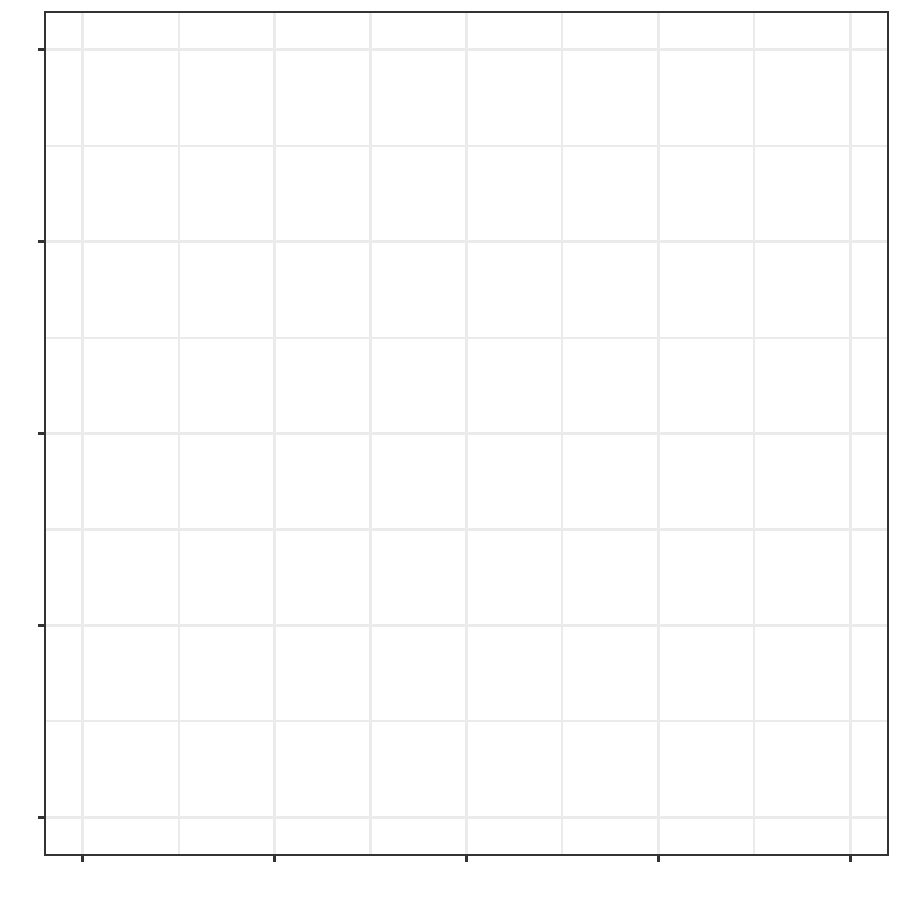
\includegraphics[width=\maxwidth]{img/desc-01-1} 

}


 
\clearpage
% -----------------------------------------------------------------------

\section{Aufgabe \hfill (7 Punkte)}

%% --------------------------------------------------------------------
\hfill\href{https://youtu.be/vXnLttRL_VI}{
\includegraphics[width =
  2cm]{img/youtube}}\\[1Ex]
%% --------------------------------------------------------------------

Nach einem Gew{\"a}chshausexperiment mit drei Bew{\"a}sserungstypen ($low$, $mid$
und $high$) ergibt sich die folgende Datentabelle mit dem gemessenen
Frischgewicht (\textit{freshmatter}).

\begin{table}[!h]
\centering
\begin{tabular}{cc}
\toprule
water\_type & freshmatter\\
\midrule
low & 22\\
high & 25\\
mid & 24\\
low & 21\\
low & 20\\
\addlinespace
low & 21\\
high & 20\\
mid & 27\\
high & 17\\
mid & 22\\
\bottomrule
\end{tabular}
\end{table}



\begin{enumerate}
\item Zeichnen Sie in \textit{einer} Abbildung die Barplots f{\"u}r die
  Bew{\"a}sserungstypen! Beschriften Sie die Achsen entsprechend!  \textbf{(4
    Punkte)}
\item Beschriften Sie \textit{einen} Barplot mit den g{\"a}ngigen
  statistischen Ma{\ss}zahlen! \textbf{(2 Punkte)}
\item Wenn Sie \textit{keinen Effekt} zwischen der Bew{\"a}sserungstypen
  erwarten w{\"u}rden, wie sehen dann die Barplots aus? \textbf{(1 Punkt)}
\end{enumerate} 
\clearpage
% -----------------------------------------------------------------------

\section{Aufgabe \hfill (6 Punkte)}

%% --------------------------------------------------------------------
\hfill\href{https://youtu.be/MiD42k4l5Ag}{
\includegraphics[width =
  2cm]{img/youtube}}\\[1Ex]
%% --------------------------------------------------------------------



\begin{enumerate}
\item Skizieren Sie in die unten stehenden, freien Abbildungen die
  Verteilungen, die sich nach der Abbildungs{\"u}berschrift ergeben! \textbf{(4
    Punkte)}
\item Achten Sie auf die entsprechende Skalierung der beiden Verteilungen
  in der ersten Abbildung! \textbf{(2 Punkte)}
\end{enumerate}



{\centering 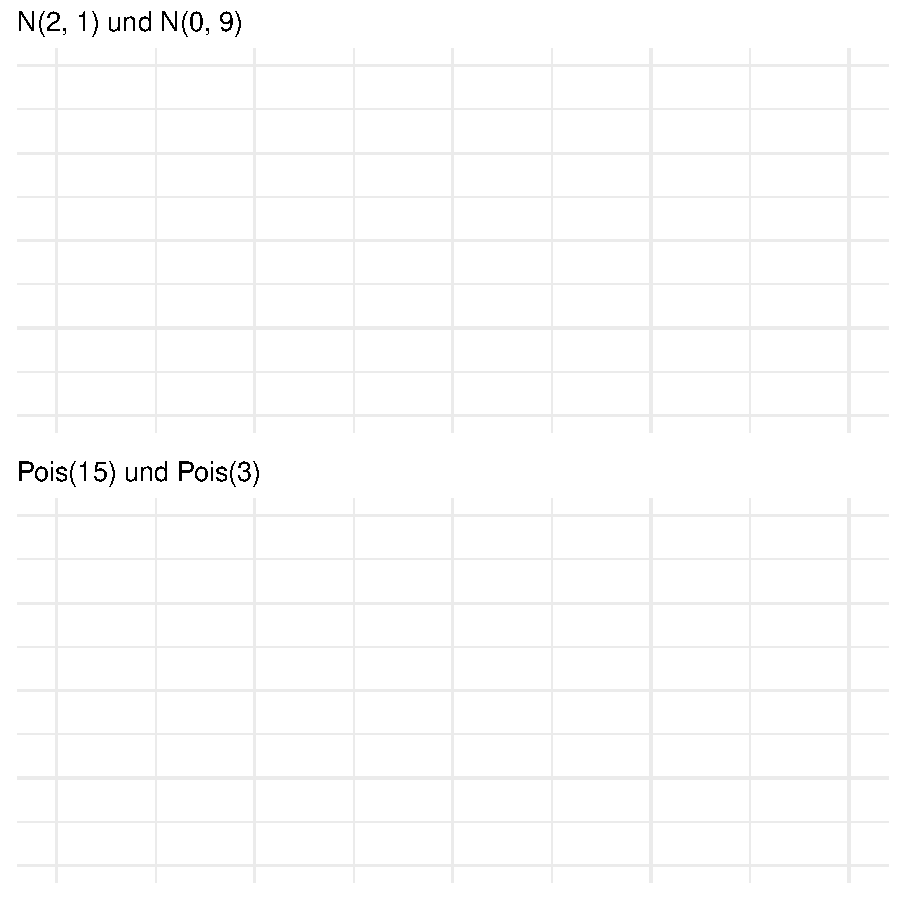
\includegraphics[width=\maxwidth]{img/histogram-01-1} 

}



 
\clearpage
% -----------------------------------------------------------------------

\section{Aufgabe \hfill (6 Punkte)}

%% --------------------------------------------------------------------
\hfill\href{https://youtu.be/ZrJhn2wPbq4}{
\includegraphics[width =
  2cm]{img/youtube}}\\[1Ex]
%% --------------------------------------------------------------------



\begin{enumerate}
\item Skizieren Sie $4$ Normalverteilungen \textit{in einer
    Abbildung} mit $\bar{y}_1 \neq \bar{y}_2 \neq \bar{y}_3 \neq \bar{y}_4$ und $s_1 = s_2 = s_3 = s_4$! \textbf{(2 Punkte)}
\item Beschriften Sie die Normalverteilungen mit den entsprechenden
  Parametern! \textbf{(2 Punkte)}
\item Liegt Varianzhomogenit{\"a}t oder Varianzheterogenit{\"a}t vor? Begr{\"u}nden Sie
  Ihre Antwort! \textbf{(2 Punkte)}
\end{enumerate}

 
\clearpage
% -----------------------------------------------------------------------

\section{Aufgabe \hfill (6 Punkte)}

%% --------------------------------------------------------------------
\hfill\href{https://youtu.be/aXvxGC4YLqk}{
\includegraphics[width =
  2cm]{img/youtube}}\\[1Ex]
%% --------------------------------------------------------------------



Nach einem Experiment z{\"a}hlen Sie folgende Anzahl an L{\"a}sionen auf den
Bl{\"a}ttern von Sonnenblumen nach einer durchgestandenen Infektion. 

\begin{center}
$2, 3, 3, 1, 3, 5, 6, 5, 2, 3, 3, 6, 5, 5$
\end{center}

\begin{enumerate}
\item Zeichen Sie ein Histogramm um die Verteilung der Daten zu visualiseren! (\textbf{3 Punkte})
\item Beschriften Sie die Achsen der Abbildung! (\textbf{2 Punkte})
\item Erg{\"a}nzen Sie die relativen H{\"a}ufigkeiten in der Abbildung! \textbf{(1
    Punkt)}  
\end{enumerate}

 
\clearpage
% -----------------------------------------------------------------------

\section{Aufgabe \hfill (8 Punkte)}

%% --------------------------------------------------------------------
\hfill\href{https://youtu.be/ORHSPTCdfeY}{
\includegraphics[width =
  2cm]{img/youtube}}\\[1Ex]
%% --------------------------------------------------------------------



Nach einem Experiment z{\"a}hlen Sie folgende Trockengewichte von Sonnenblumen nach einer durchgestandenen Infektion. 

\begin{center}
$11.5, 7.1, 11.2, 8.4, 9.8, 10.6, 10.1, 11.6, 11, 9.6, 14.1, 11.4, 9.8, 14, 8.1$
\end{center}

\begin{enumerate}
\item Zeichen Sie ein Histogramm um die Verteilung der Daten zu
  visualiseren! (\textbf{3 Punkte})
 \item Erl{\"a}utern Sie Ihr Vorgehen um ein Histogramm f{\"u}r kontinuierliche
  Daten zu zeichnen!  (\textbf{2 Punkte})
\item Beschriften Sie die Achsen der Abbildung! (\textbf{2 Punkte})
\item Erg{\"a}nzen Sie die relativen H{\"a}ufigkeiten in der Abbildung! \textbf{(1
    Punkt)}  
\end{enumerate}

 
\clearpage
% -----------------------------------------------------------------------

\section{Aufgabe \hfill (9 Punkte)}

%% --------------------------------------------------------------------
\hfill\href{https://youtu.be/0xc0jIPeiyw}{
\includegraphics[width =
  2cm]{img/youtube}}\\[1Ex]
%% --------------------------------------------------------------------


Nach einem Feldexperiment mit zwei D{\"u}ngestufen (A und B) ergibt sich die
folgende Datentabelle mit dem gemessenen Trockengewicht (\textit{drymatter}). 

\begin{table}[!h]
\centering
\begin{tabular}{cc}
\toprule
trt & drymatter\\
\midrule
A & 13.8\\
A & 7.5\\
B & 15.3\\
A & 7.7\\
A & 9.4\\
\addlinespace
A & 9.4\\
A & 1.8\\
B & 12.6\\
B & 20.6\\
A & 14.8\\
\addlinespace
B & 12.0\\
B & 14.9\\
B & 11.9\\
B & 12.8\\
A & 10.6\\
\addlinespace
A & 9.4\\
A & 14.7\\
A & 9.8\\
\bottomrule
\end{tabular}
\end{table}



\begin{enumerate}
\item Zeichnen Sie in \textit{einer} Abbildung die beiden Boxplots f{\"u}r die
  zwei D{\"u}ngestufen A und B! Beschriften Sie die Achsen entsprechend!
  \textbf{(6 Punkte)}
\item Beschriften Sie \textit{einen} der beiden Boxplots mit den g{\"a}ngigen
  statistischen Ma{\ss}zahlen! \textbf{(2 Punkte)}
\item Wenn Sie \textit{keinen Effekt} zwischen den D{\"u}ngestufen erwarten
  w{\"u}rden, wie sehen dann die beiden Boxplots aus? \textbf{(1 Punkt)}
\end{enumerate} 
\clearpage
% -----------------------------------------------------------------------

\section{Aufgabe \hfill (9 Punkte)}

%% --------------------------------------------------------------------
\hfill\href{https://youtu.be/VX4Hs81h8_A}{
\includegraphics[width =
  2cm]{img/youtube}}\\[1Ex]
%% --------------------------------------------------------------------

Nach einem Feldexperiment mit mehreren D{\"u}ngestufen stellt sich die Frage,
ob die D{\"u}ngestufe \textit{low} im Bezug auf das Trockengewicht
normalverteilt sei. Sie erhalten folgende Datentabelle.

\begin{table}[!h]
\centering
\begin{tabular}{cc}
\toprule
fertilizer & drymatter\\
\midrule
low & 24\\
low & 17\\
low & 22\\
low & 23\\
low & 19\\
\addlinespace
low & 25\\
low & 21\\
\bottomrule
\end{tabular}
\end{table}



\begin{enumerate}
\item Zeichnen Sie eine passende Abbildung in der Sie visuell {\"u}berpr{\"u}fen
  k{\"o}nnen, ob eine Normalverteilung des Trockengewichts vorliegt! \textbf{(4
    Punkte)}
\item Beschriften Sie die Achsen und erg{\"a}nzen Sie die statistischen
  Ma{\ss}zahlen. \textbf{(3 Punkte)}
\item Entscheiden Sie, ob eine Normalveteilung vorliegt. Begr{\"u}nden Sie Ihre
  Antwort. \textbf{(2 Punkte)}
\end{enumerate} 
\clearpage
% -----------------------------------------------------------------------

\section{Aufgabe \hfill (4 Punkte)}

%% --------------------------------------------------------------------
\hfill\href{https://youtu.be/Op-gjzASH9I}{
\includegraphics[width =
  2cm]{img/youtube}}\\[1Ex]
%% --------------------------------------------------------------------



\begin{enumerate}
\item Zeichnen Sie {\"u}ber den untenstehenden Boxplot die entsprechende
  zugeh{\"o}rige Verteilung! \textbf{(2 Punkte)} 
\item Zeichnen Sie unter den untenstehenden Boxplot die entsprechende
  zugeh{\"o}rige Beobachtungen! \textbf{(2 Punkte)}
\end{enumerate}

\vspace*{8cm}

\begin{center}
  
\includegraphics[width=10cm]{/Users/kruppajo/Documents/GitHub/exam/question/img/boxplot-03-c.png}
\end{center}



 
\clearpage
% -----------------------------------------------------------------------

\section{Aufgabe \hfill (9 Punkte)}

%% --------------------------------------------------------------------
\hfill\href{https://youtu.be/lXI_H6m26HE}{
\includegraphics[width =
  2cm]{img/youtube}}\\[1Ex]
%% --------------------------------------------------------------------


In einem Experiment mit zwei D{\"u}ngestufen f{\"u}r den Ertrag von Kichererbsen
ergibt sich folgende Abbildung. 





{\centering 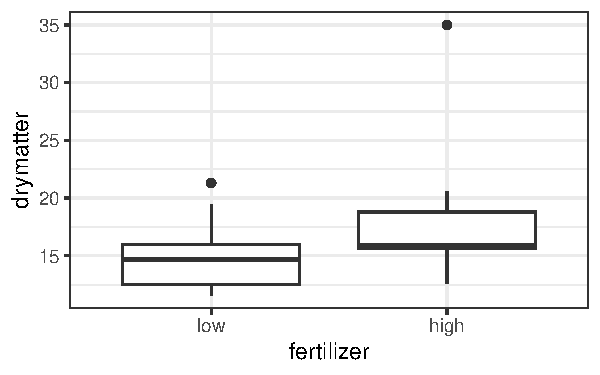
\includegraphics[width=\maxwidth]{img/boxplot-4b-1} 

}




\begin{enumerate}
\item Tragen Sie in die untenstehende Tabelle die g{\"a}ngigen Ma{\ss}zahlen des
  Boxplots und die abgesch{\"a}tzen Werte aus den obigen Boxplots ein! \textbf{(4 Punkte)}
\end{enumerate}

\begin{center}
  \large
  \begin{tabular}[c]{c|c|c}
    Statistische Ma{\ss}zahl  & \multicolumn{2}{c}{Abgesch{\"a}tzter Wert}  \strut\\
    & low & high \\
    \hline
    \hspace{2cm} & \hspace{2cm} & \hspace{2cm} \strut\\
    \hline
    \hspace{2cm} & \hspace{2cm} & \hspace{2cm} \strut\\
    \hline
    \hspace{2cm} & \hspace{2cm} & \hspace{2cm} \strut\\
    \hline
    \hspace{2cm} & \hspace{2cm} & \hspace{2cm} \strut\\
    \hline
    \hspace{2cm} & \hspace{2cm} & \hspace{2cm} \strut\\
    \hline
  \end{tabular}
\end{center}


\begin{enumerate}
  \setcounter{enumi}{1}
\item Erg{\"a}nzen Sie den Mittelwert f{\"u}r beide Level des D{\"u}ngers in die
  Abbildung der Boxplots! Begr{\"u}nden Sie Ihre Antwort! \textbf{(2 Punkte)}
\item Erg{\"a}nzen Sie in der untenstehenden Tabelle die $p$-Werte f{\"u}r den
  Shapiro-Wilk-Test auf Normalverteilung und den Levene-Test auf
  Varianzhomogenit{\"a}t. Beachten Sie die unterschiedliche, angenommene
  Fallzahl $n_g$ der beiden Level des D{\"u}ngers! \textbf{(3 Punkte)}
\end{enumerate}

\begin{center}
  \large
  \begin{tabular}[c]{l|c|c}
  Fallzahl  & Shapiro-Wilk-Test & Levene-Test \strut\\ 
    \hline
    \textbf{$n_g = 5$} & \hspace{4cm} & \hspace{4cm} \strut\\
    \hline
    \textbf{$n_g = 20$} & \hspace{4cm} & \hspace{4cm} \strut\\
    \hline
    \textbf{$n_g > 50$} & \hspace{4cm} & \hspace{4cm} \strut\\
    \hline
  \end{tabular}
\end{center} 
\clearpage
% -----------------------------------------------------------------------

\section{Aufgabe \hfill (6 Punkte)}

%% --------------------------------------------------------------------
\hfill\href{https://youtu.be/knAziLLQGb0}{
\includegraphics[width =
  2cm]{img/youtube}}\\[1Ex]
%% --------------------------------------------------------------------

Nach einer Bonitur von Schnittlauch mit einer Kontrolle und drei Pestiziden (ctrl, pestKill, roundUp, zeroX) ergibt sich die folgende Datentabelle mit den Boniturnoten (\textit{grade}). 

\begin{table}[!h]
\centering
\begin{tabular}{cc}
\toprule
pesticide & grade\\
\midrule
roundUp & 2\\
ctrl & 6\\
roundUp & 3\\
ctrl & 5\\
zeroX & 2\\
\addlinespace
zeroX & 2\\
pestKill & 3\\
ctrl & 6\\
zeroX & 2\\
ctrl & 6\\
\addlinespace
pestKill & 2\\
roundUp & 5\\
pestKill & 1\\
zeroX & 1\\
roundUp & 2\\
\bottomrule
\end{tabular}
\end{table}



\begin{enumerate}
\item Zeichnen Sie in \textit{einer} Abbildung die Dotplots f{\"u}r die
  vier Pestizidlevel! Beschriften Sie die Achsen entsprechend!
  \textbf{(4 Punkte)}
\item Erg{\"a}nzen Sie die Dotplots mit der g{\"a}ngigen
  statistischen Ma{\ss}zahl. \textbf{(1 Punkt)}
\item Wenn Sie \textit{keinen Effekt} zwischen den Pestizidlevel erwarten
  w{\"u}rden, wie sehen dann die Dotplots aus? \textbf{(1 Punkt)}
\end{enumerate} 
\clearpage
% -----------------------------------------------------------------------

\section{Aufgabe \hfill (8 Punkte)}

%% --------------------------------------------------------------------
\hfill\href{https://youtu.be/t_1KL77mfmg}{
\includegraphics[width =
  2cm]{img/youtube}}\\[1Ex]
%% --------------------------------------------------------------------

Nach einem Feldexperiment mit zwei Pestiziden (\textit{RoundUp} und
\textit{OutEx}) ergibt sich die folgende Datentabelle mit dem jeweiligen
beobachteten Infektionsstatus.

\begin{table}[!h]
\centering
\begin{tabular}{cc}
\toprule
pesticide & infected\\
\midrule
RoundUp & yes\\
OutEx & no\\
OutEx & yes\\
RoundUp & no\\
RoundUp & yes\\
\addlinespace
RoundUp & yes\\
RoundUp & yes\\
OutEx & no\\
OutEx & no\\
RoundUp & yes\\
\addlinespace
OutEx & yes\\
RoundUp & yes\\
RoundUp & no\\
RoundUp & yes\\
OutEx & no\\
\addlinespace
RoundUp & yes\\
OutEx & no\\
OutEx & no\\
OutEx & yes\\
OutEx & yes\\
\addlinespace
RoundUp & yes\\
OutEx & yes\\
\bottomrule
\end{tabular}
\end{table}



\begin{enumerate}
\item Stellen Sie in einer 2x2 Tafel den Zusammenhang zwischen dem
  Pesizid und dem Infektionsstatus dar! \textbf{(4 Punkte)}
\item Zeichnen Sie den zugeh{\"o}rigen Mosaic-Plot. Berechnen Sie das
  Verh{\"a}ltnis pro Spalte! \textbf{(2 Punkte)}
\item Wenn das Pesizid keine Auswirkung auf den Infektionsstatus h{\"a}tte, wie
  sehe dann der Mosaic-Plot aus? \textbf{(2 Punkte)}
\end{enumerate} 
\clearpage
% -----------------------------------------------------------------------

\section{Aufgabe \hfill (10 Punkte)}

%% --------------------------------------------------------------------
\hfill\href{https://youtu.be/VAqiUdV4WQ0}{
\includegraphics[width =
  2cm]{img/youtube}}\\[1Ex]
%% --------------------------------------------------------------------

In einem Feldexperiment f{\"u}r die Bodendurchl{\"a}ssigkeit wurde der Niederschlag
pro Parzelle sowie der durchschnittliche Ertrag gemessen. Es ergibt sich
folgende Datentabelle. 

\begin{table}[!h]
\centering
\begin{tabular}{cc}
\toprule
water & drymatter\\
\midrule
20 & 15\\
17 & 17\\
32 & 21\\
31 & 24\\
22 & 18\\
\bottomrule
\end{tabular}
\end{table}



\begin{enumerate}
\item Erstellen Sie den Scatter-Plot f{\"u}r die Datentabelle. Beschriften Sie
  die Achsen entsprechend! \textbf{(4 Punkte)}
\item Zeichnen Sie eine Gerade durch die Punkte! \textbf{(1 Punkt)}
\item Beschriften Sie die Gerade mit den g{\"a}ngigen statistischen Ma{\ss}zahlen! \textbf{(3 Punkte)}
\item Wenn kein Effekt von dem Niederschlag auf das Trockengewicht
  vorhanden w{\"a}re, wie w{\"u}rde die Gerade verlaufen und welche Werte w{\"u}rden die
  statistischen Ma{\ss}zahlen annehmen? \textbf{(2 Punkt)}
\end{enumerate} 
\clearpage
% -----------------------------------------------------------------------
\begin{graybox}{Statistisches Testen}
Mehr Informationen zu den Aufgaben in den folgenden Kapiteln aus dem Skript Bio Data Science.
  \begin{itemize}
  \item \href{https://jkruppa.github.io/preface.html#lernziel-3-falsifikationsprinzip}{Kapitel 3 - Falsifikationsprinzip}
  \item \href{https://jkruppa.github.io/stat-tests-basic.html}{Kapitel 19 - Die Testentscheidung}
  \item \href{https://jkruppa.github.io/stat-tests-theorie.html}{Kapitel 20 - Die Testtheorie}
  \end{itemize}
\end{graybox}
\clearpage
% -----------------------------------------------------------------------  

\section{Aufgabe \hfill (6 Punkte)}

%% --------------------------------------------------------------------
\hfill\href{https://youtu.be/1S-FuQisTpE}{
\includegraphics[width =
  2cm]{img/youtube}}\\[1Ex]
%% --------------------------------------------------------------------

\begin{enumerate}
\item Erkl{\"a}ren Sie den Zusammenhang zwischen Stichprobe und Grundgesamtheit
  an einem Schaubild! \textbf{(3 Punkte)}
\item Was ist der Unterschied zwischen $\mu$ und $\sigma$ und $\bar{y}$ und
  $s$ im Kontext der Stichprobe und Grundgesamtheit? \textbf{(2 Punkte)}
\item Warum m{\"u}ssen wir {\"u}berhaupt zwischen einer Stichprobe und einer
  Grundgesamtheit unterscheiden? \textbf{(1 Punkt)}
\end{enumerate} 
\clearpage
% -----------------------------------------------------------------------

\section{Aufgabe \hfill (8 Punkte)}

%% --------------------------------------------------------------------
\hfill\href{https://youtu.be/3DfWs9NNrCk}{
\includegraphics[width =
  2cm]{img/youtube}}\\[1Ex]
%% --------------------------------------------------------------------




Geben ist folgende 2x2 Kreuztabelle. 

\begin{center}
  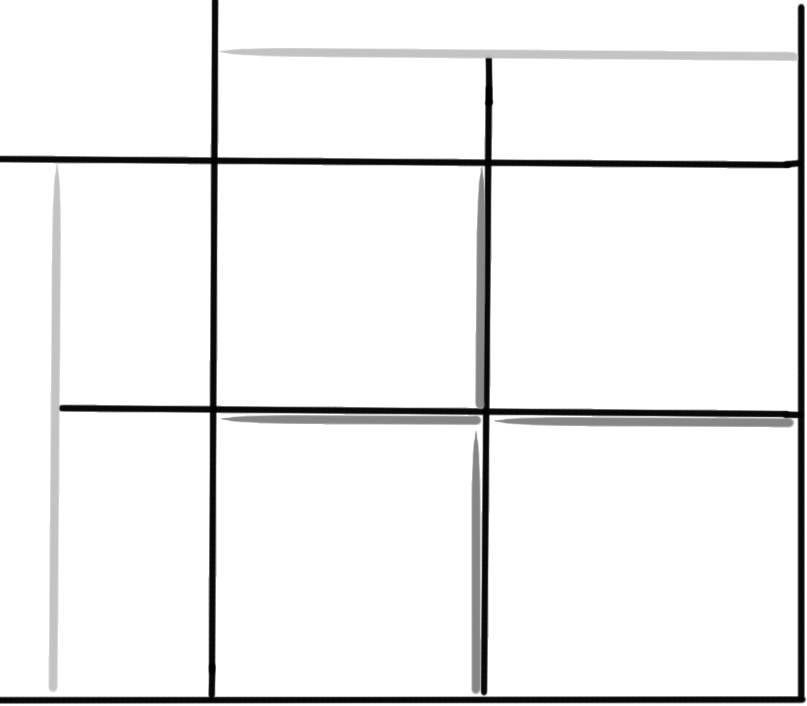
\includegraphics[width = 13cm]{/Users/kruppajo/Documents/GitHub/exam/question/img/text-error-cross-table}
\end{center}

\begin{enumerate}
\item Tragen Sie folgende Fachbegriffe korrekt in die 2x2 Kreuztabelle ein! \textbf{(4 Punkte)}
  \begin{itemize}
  \item (Unbekannte) Wahrheit	
  \item H$_0$ wahr
  \item H$_0$ falsch
  \item H$_0$ abgelehnt
  \item H$_0$ beibehalten
  \item Testentscheidung
  \item $\alpha$-Fehler
  \item $\beta$-Fehler
  \item Richtige Entscheidung
  \item 5\%
  \item 20\%
  \end{itemize}
\item In der Analogie des Feuermelders, wie lauetet der $\alpha$-Fehler? \textbf{(1 Punkt)}
\item In der Analogie des Feuermelders, wie lauetet der $\beta$-Fehler? \textbf{(1 Punkt)}
\item Wenn der Feuermelder einmal pro Tag messen w{\"u}rde, wie oft w{\"u}rde der
  Feuermelder mit einem $\alpha$ von 5\% in einem Monat Alarm schlagen?
  Begr{\"u}nden Sie Ihre Antwort! \textbf{(2 Punkte)}
\end{enumerate}



 
\clearpage
% -----------------------------------------------------------------------

\section{Aufgabe \hfill (8 Punkte)}

%% --------------------------------------------------------------------
\hfill\href{https://youtu.be/32JjH1eyuTU}{
\includegraphics[width =
  2cm]{img/youtube}}\\[1Ex]
%% --------------------------------------------------------------------



Im folgenden ist eine t-Verteilung abgebildet. Erg{\"a}nzen Sie die Abbildung wie folgt.

\begin{enumerate}
\item Zeichnen Sie das Signifikanzniveau $\alpha$ in die Abbildung! \textbf{(2 Punkte)} 
\item Zeichnen Sie einen signifikant p-Wert in die Abbildung! \textbf{(2 Punkte)} 
\item Erg{\"a}nzen Sie "`$\bar{y}_1 = \bar{y}_2$"'! \textbf{(1 Punkt)} 
\item Erg{\"a}nzen Sie "`$A = 0.95$"'! \textbf{(1 Punkt)}
\item Zeichnen Sie $T_{\alpha=5\%}$ in die Abbildung! \textbf{(1 Punkt)} 
\item Zeichnen Sie $+T_{calc}$ in die Abbildung! \textbf{(1 Punkt)} 
\end{enumerate}



{\centering 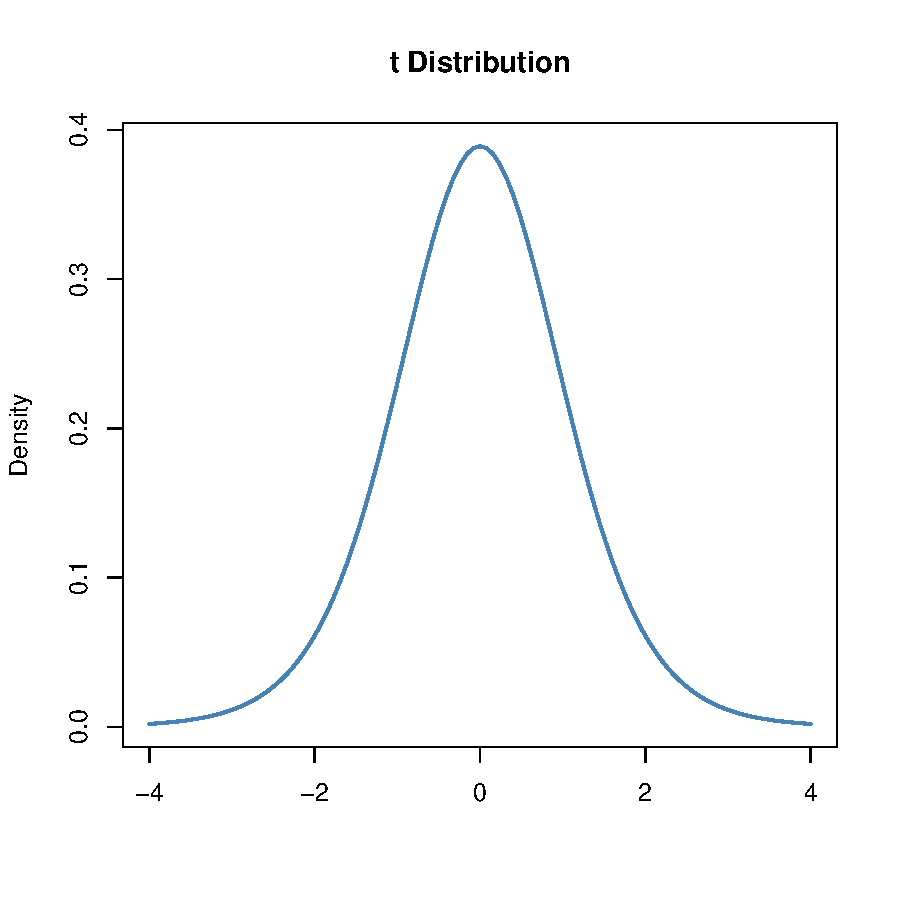
\includegraphics[width=\maxwidth]{img/statistisches-testen-3-1} 

}


 
\clearpage
% -----------------------------------------------------------------------

\section{Aufgabe \hfill (10 Punkte)}

%% --------------------------------------------------------------------
\hfill\href{https://youtu.be/CN_O4fYPbhs}{
\includegraphics[width =
  2cm]{img/youtube}}\\[1Ex]
%% --------------------------------------------------------------------



Sie rechnen einen t-Test f{\"u}r Gruppenvergleiche. Sie sch{\"a}tzen den Unterschied
zwischen dem mittleren Trockengewicht nach D{"u}ngergabe. 

\begin{enumerate}
\item Beschriften Sie die untenstehende Abbildung mit der
  Signifikanzschwelle! Begr{\"u}nden Sie Ihre Antwort! \textbf{(2 Punkte)}
\item Erg{\"a}nzen Sie eine \textit{in den Kontext passende} Relevanzschwelle!
  Begr{\"u}nden Sie Ihre Antwort! \textbf{(2 Punkte)} 
\item Skizieren Sie in die
  untenstehende Abbildung sechs einzelne Konfidenzintervalle (a-f) mit den
  jeweiligen Eigenschaften! \textbf{(6 Punkte)}
  \begin{itemize}
  \item[(a)] Ein signifikantes, nicht relevantes 95\%-Konfidenzintervall 	
  \item[(b)] Ein signifikantes, relevantes 95\%-Konfidenzintervall 	
  \item[(c)] Ein 95\%-Konfidenzintervall mit niedriger Varianz $s_p$ in der Stichprobe als der Rest 95\%-der Konfidenzintervalle 	
  \item[(d)] Ein 95\%-Konfidenzintervall mit h{"o}herer Varianz $s_p$ in der Stichprobe als der Rest der 95\%-Konfidenzintervalle 
  \item[(e)] Ein nicht signifikantes, nicht relevantes 95\%-Konfidenzintervall
  \item[(f)] Ein signifikantes, relevantes 90\%-Konfidenzintervall.
  \end{itemize}
\end{enumerate}

\begin{center}
  
\includegraphics[height = 8cm]{/Users/kruppajo/Documents/GitHub/exam/question/img/statistisches-testen-04}
\end{center}


 
\clearpage
% -----------------------------------------------------------------------

\section{Aufgabe \hfill (6 Punkte)}

%% --------------------------------------------------------------------
\hfill\href{https://youtu.be/bc1m7rkXld4}{
\includegraphics[width =
  2cm]{img/youtube}}\\[1Ex]
%% --------------------------------------------------------------------

Gegeben ist die vereinfachte Formel f{\"u}r den Zweistichproben t-Test mit der
gepoolten Standardabweichung $s_p$ und gleicher Gruppengr{\"o}sse $n_g$ der
beiden Sample.

\begin{equation*}
  \label{eq:1}
  T = \cfrac{\bar{y}_1 - \bar{y}_2}{s_p \cdot \sqrt{\tfrac{2}{n_g}}}
\end{equation*}

Welche Auswirkung hat die {\"A}nderungen der jeweiligen statistischen Masszahl
auf den T-Wert und damit auf die \textit{vermutliche} Signifikanz? F{\"u}llen
Sie hierzu die untenstehende Tabelle aus! \textbf{(6 Punkte)}

\begin{center}
  \large
  \begin{tabular}[c]{l|l|l|l|l|l|l|l}
    & T Statistik & $Pr(D|H_0)$ & $KI_{1-\alpha}$ & & T Statistik & $Pr(D|H_0)$ & $KI_{1-\alpha}$\strut\\ 
    \hline
    \textbf{$\Delta\; \uparrow$} & \hspace{2cm} & \hspace{2cm}  & \hspace{2cm} & \textbf{
                                                          $\Delta\; \downarrow$} &
                                                                          \hspace{2cm} & \hspace{2cm}  & \hspace{2cm}\strut\\
    \hline
        \textbf{$s\; \uparrow$} & \hspace{2cm} & \hspace{2cm}  & \hspace{2cm} & \textbf{
                                                          $s\; \downarrow$} &
                                                                          \hspace{2cm}
                                                & \hspace{2cm}  & \hspace{2cm}\strut\\
    \hline
        \textbf{$n\; \uparrow$} & \hspace{2cm} & \hspace{2cm}  & \hspace{2cm} & \textbf{
                                                          $n\; \downarrow$} &
                                                                          \hspace{2cm}
                                                & \hspace{2cm}  & \hspace{2cm}\strut\\
    \hline
  \end{tabular}
\end{center}
 
\clearpage
% -----------------------------------------------------------------------

\section{Aufgabe \hfill (8 Punkte)}

%% --------------------------------------------------------------------
\hfill\href{https://youtu.be/gQwvMuZ-Sjs}{
\includegraphics[width =
  2cm]{img/youtube}}\\[1Ex]
%% --------------------------------------------------------------------



Sie haben folgende Aussage gegeben.

\begin{center}
  \Large\textbf{Bin ich im Winter?}
\end{center}

\begin{enumerate}
\item Erkl{\"a}ren Sie den Gedankengang der Testtheorie sowie des Falsifikationsprinzips an der Aussage! \textbf{(4 Punkte)}
\item Erkl{\"a}ren Sie Ihre Entscheidung zu der Aussage! \textbf{(3 Punkte)}
\item Sch{\"a}tzen Sie den p-Wert zu der Aussage ab! \textbf{(1 Punkt)}
\end{enumerate}

 
\clearpage
% -----------------------------------------------------------------------
\begin{graybox}{Der t-Test}
Mehr Informationen zu den Aufgaben in den folgenden Kapiteln aus dem Skript Bio Data Science.
  \begin{itemize}
  \item \href{https://jkruppa.github.io/stat-tests-ttest.html}{Kapitel 22 - Der t-Test}
  \end{itemize}
\end{graybox}
\clearpage
% -----------------------------------------------------------------------

\section{Aufgabe \hfill (12 Punkte)}

%% --------------------------------------------------------------------
\hfill\href{https://youtu.be/Cq_rF_z4xOk}{
\includegraphics[width =
  2cm]{img/youtube}}\\[1Ex]
%% --------------------------------------------------------------------

Nach einem Experiment mit zwei Pestiziden (\textit{RoundUp} und
\textit{GoneEx}) ergibt sich die folgende Datentabelle mit dem gemessenen
Trockengewicht (\textit{drymatter}) von Weizen.

\begin{table}[!h]
\centering
\begin{tabular}{cc}
\toprule
pesticide & drymatter\\
\midrule
RoundUp & 17\\
GoneEx & 15\\
RoundUp & 16\\
RoundUp & 18\\
GoneEx & 19\\
\addlinespace
GoneEx & 18\\
GoneEx & 16\\
RoundUp & 17\\
RoundUp & 17\\
RoundUp & 15\\
\addlinespace
GoneEx & 17\\
RoundUp & 16\\
\bottomrule
\end{tabular}
\end{table}



\begin{enumerate}
  \item Formulieren Sie die wissenschaftliche Fragestellung! \textbf{(1 Punkt)}
  \item Formulieren Sie das statistische Hypothesenpaar! \textbf{(2
      Punkte)}
  \item Bestimmen Sie die Teststatistik $T_{calc}$ eines Student t-Tests f{\"u}r den
  Vergleich der beiden Pestizide. Geben Sie den Rechenweg und die Formeln
  mit an! \textbf{(5 Punkte)}
\item Treffen Sie mit $T_{\alpha = 5\%} = 2.04$ und dem berechneten $T_{calc}$ eine Aussage
  zur Nullhypothese! \textbf{(2 Punkte)}
\item Wenn Sie keinen Unterschied zwischen den beiden Pestiziden erwarten
  w{\"u}rden, wie gro{\ss}e w{\"a}re dann die Teststatistik $T_{calc}$? Begr{\"u}nden Sie Ihre
  Antwort! \textbf{(2 Punkte)}
\end{enumerate} 
\clearpage
% -----------------------------------------------------------------------

\section{Aufgabe \hfill (13 Punkte)}

%% --------------------------------------------------------------------
\hfill\href{https://youtu.be/QR90zyn0Iz8}{
\includegraphics[width =
  2cm]{img/youtube}}\\[1Ex]
%% --------------------------------------------------------------------


Das Gewicht von K{\"u}ken wurde \textit{vor} der Behandlung mit STARTex und 1
Woche \textit{nach} der Behandlung gemessen. Es ergibt sich die folgende
Datentabelle.

\begin{table}[!h]
\centering
\begin{tabular}{ccc}
\toprule
animal\_id & before & after\\
\midrule
1 & 10 & 14\\
2 & 12 & 11\\
3 & 5 & 15\\
4 & 22 & 10\\
5 & 13 & 12\\
\addlinespace
6 & 18 & 10\\
7 & 11 & 12\\
8 & 17 & 13\\
9 & 8 & 11\\
\bottomrule
\end{tabular}
\end{table}



\begin{enumerate}
\item Formulieren Sie die Fragestellung! \textbf{(1 Punkt)}
\item Formulieren Sie das statistische Hypothesenpaar! \textbf{(2
    Punkte)}
\item Bestimmen Sie die Teststatistik $T_{calc}$ eines gepaarten t-Tests f{\"u}r den
  Vergleich der beiden Zeitpunkte. Geben Sie den Rechenweg und die Formeln
  mit an! \textbf{(4 Punkte)}
\item Treffen Sie mit $T_{\alpha = 5\%} = 2.04$ und dem berechneten $T_{calc}$ eine Aussage
  zur Nullhypothese! \textbf{(2 Punkte)}
\item Wenn Sie keinen Unterschied zwischen den beiden Zeitpunkten erwarten
  w{\"u}rden, wie gro{\ss}e w{\"a}re dann die Teststatistik $T_{calc}$? Begr{\"u}nden Sie Ihre
  Antwort! \textbf{(2 Punkte)}
\item Sch{\"a}tzen Sie $Pr(D|H_0)$ ab. Begr{\"u}nden Sie Ihre Antwort! \textbf{(2
    Punkte)}
\end{enumerate} 
\clearpage
% -----------------------------------------------------------------------

\section{Aufgabe \hfill (10 Punkte)}

%% --------------------------------------------------------------------
\hfill\href{https://youtu.be/exDo7AyHl4Q}{
\includegraphics[width =
  2cm]{img/youtube}}\\[1Ex]
%% --------------------------------------------------------------------

Sie erhalten folgende \Rlogo Ausgabe der Funktion \texttt{t.test()}.

\begin{knitrout}
\definecolor{shadecolor}{rgb}{0.969, 0.969, 0.969}\color{fgcolor}\begin{kframe}
\begin{verbatim}
## 
## 	Two Sample t-test
## 
## data:  waterintake by infusion
## t = -0.70711, df = 10, p-value = 0.4956
## alternative hypothesis: true difference in means between group high and group low is not equal to 0
## 95 percent confidence interval:
##  -3.558055  1.843769
## sample estimates:
## mean in group ctrl mean in group trt1 
##           17.14286           18.00000
\end{verbatim}
\end{kframe}
\end{knitrout}


\begin{enumerate}
  \item Formulieren Sie das statistische Hypothesenpaar! \textbf{(2
Punkte)}
\item Liegt ein signifikanter Unterschied zwischen den Gruppen vor?
  Begr{\"u}nden Sie Ihre Antwort! \textbf{(2 Punkte)}
\item Skizieren Sie eine Abbildung in der Sie $T_{calc}$, $Pr(D|H_0)$, $A=0.95$,
  sowie $T_{\alpha=5\%} = |2.23|$ einzeichnen! \textbf{(4 Punkte)}
\item Beschriften Sie die Abbildung entsprechend! \textbf{(2 Punkte)}  
\end{enumerate} 
\clearpage
% -----------------------------------------------------------------------

\section{Aufgabe \hfill (8 Punkte)}

%% --------------------------------------------------------------------
\hfill\href{https://youtu.be/wJqsNV1hOW8}{
\includegraphics[width =
  2cm]{img/youtube}}\\[1Ex]
%% --------------------------------------------------------------------

Sie erhalten folgende \Rlogo Ausgabe der Funktion \texttt{t.test()}.

\begin{knitrout}
\definecolor{shadecolor}{rgb}{0.969, 0.969, 0.969}\color{fgcolor}\begin{kframe}
\begin{verbatim}
## 
## 	Two Sample t-test
## 
## data:  freshmatter by N
## t = 2.5664, df = 12, p-value = 0.02471
## alternative hypothesis: true difference in means between group high and group low is not equal to 0
## 95 percent confidence interval:
##  0.5571471 6.8206307
## sample estimates:
## mean in group ctrl  mean in group low 
##           17.80000           14.11111
\end{verbatim}
\end{kframe}
\end{knitrout}


\begin{enumerate}
  \item Formulieren Sie das statistische Hypothesenpaar! \textbf{(2
Punkte)}
\item Liegt ein signifikanter Unterschied zwischen den Gruppen vor?
  Begr{\"u}nden Sie Ihre Antwort! \textbf{(2 Punkte)}
\item Skizieren Sie das sich ergebende 95\% Konifidenzintervall! \textbf{(2 Punkte)}
\item Beschriften Sie die Abbildung und
  das 95\% Konfidenzintervall entsprechend! \textbf{(2 Punkte)}  
\end{enumerate} 
\clearpage
% -----------------------------------------------------------------------

\section{Aufgabe \hfill (8 Punkte)}

%% --------------------------------------------------------------------
\hfill\href{https://youtu.be/w62HJlbN28U}{
\includegraphics[width =
  2cm]{img/youtube}}\\[1Ex]
%% --------------------------------------------------------------------

Sie erhalten folgende \Rlogo Ausgabe der Funktion \texttt{t.test()}.

\begin{knitrout}
\definecolor{shadecolor}{rgb}{0.969, 0.969, 0.969}\color{fgcolor}\begin{kframe}
\begin{verbatim}
## 
## 	Two Sample t-test
## 
## data:  waterintake by infusion
## t = -0.94868, df = 8, p-value = 0.3706
## alternative hypothesis: true difference in means between group high and group low is not equal to 0
## 95 percent confidence interval:
##  -4.11689  1.71689
## sample estimates:
## mean in group high mean in group trt2 
##               16.6               17.8
\end{verbatim}
\end{kframe}
\end{knitrout}


\begin{enumerate}
  \item Formulieren Sie das statistische Hypothesenpaar! \textbf{(2
Punkte)}
\item Liegt ein signifikanter Unterschied zwischen den Gruppen vor?
  Begr{\"u}nden Sie Ihre Antwort! \textbf{(2 Punkte)}
\item Skizieren Sie die sich ergebenden Boxplots! Welche Annahmen an die Daten haben Sie getroffen? Begr{\"u}nden Sie Ihre Antwort! \textbf{(4 Punkte)} 
\end{enumerate}
 
\clearpage
% -----------------------------------------------------------------------

\section{Aufgabe \hfill (8 Punkte)}

%% --------------------------------------------------------------------
\hfill\href{https://youtu.be/kHmfEmU6lrk}{
\includegraphics[width =
  2cm]{img/youtube}}\\[1Ex]
%% --------------------------------------------------------------------


Sie erhalten folgende \Rlogo Ausgabe der Funktion \texttt{t.test()}.

\begin{knitrout}
\definecolor{shadecolor}{rgb}{0.969, 0.969, 0.969}\color{fgcolor}\begin{kframe}
\begin{verbatim}
## 
## 	Paired t-test
## 
## data:  waterintake by infusion
## t = -2.4087, df = 4, p-value = 0.07366
## alternative hypothesis: true mean difference is not equal to 0
## 95 percent confidence interval:
##  -13.777198   0.977198
## sample estimates:
## mean difference 
##            -6.4
\end{verbatim}
\end{kframe}
\end{knitrout}


\begin{enumerate}
  \item Formulieren Sie die wissenschaftliche Fragestellung! \textbf{(2
Punkte)}
\item Liegt ein signifikanter Unterschied zwischen den Gruppen vor?
  Begr{\"u}nden Sie Ihre Antwort! \textbf{(2 Punkte)}
\item Skizzieren Sie den sich ergebenden Datensatz mit $n = 4$
  Beobachtungen! Die Daten m{\"u}ssen \textit{nicht} die Mittelwertsdifferenz
  $d$ erf{\"u}llen! \textbf{(2 Punkte)} 
\item Skizieren Sie den sich ergebenden Boxplot der Differenzen! Welche Annahmen an die Daten haben Sie getroffen? Begr{\"u}nden Sie Ihre Antwort! \textbf{(2 Punkte)} 
\end{enumerate}
 
\clearpage
% -----------------------------------------------------------------------
\begin{graybox}{Die ANOVA}
Mehr Informationen zu den Aufgaben in den folgenden Kapiteln aus dem Skript Bio Data Science.
  \begin{itemize}
  \item \href{https://jkruppa.github.io/stat-tests-anova.html}{Kapitel 23 - Die ANOVA}
  \end{itemize}
\end{graybox}
\clearpage
% -----------------------------------------------------------------------

\section{Aufgabe \hfill (8 Punkte)}

%% --------------------------------------------------------------------
\hfill\href{https://youtu.be/Q7xtQJoOmQI}{
\includegraphics[width =
  2cm]{img/youtube}}\\[1Ex]
%% --------------------------------------------------------------------

In einem Experiment wurde der Ertrag von Erbsen unter drei verschiedenen
Pestizid-Dosen 0.5 g/l, 1.5 g/l und 2.5 g/l gemessen. Unten stehenden sehen
Sie die Visualisierung des Datensatzes.

\begin{knitrout}
\definecolor{shadecolor}{rgb}{0.969, 0.969, 0.969}\color{fgcolor}

{\centering 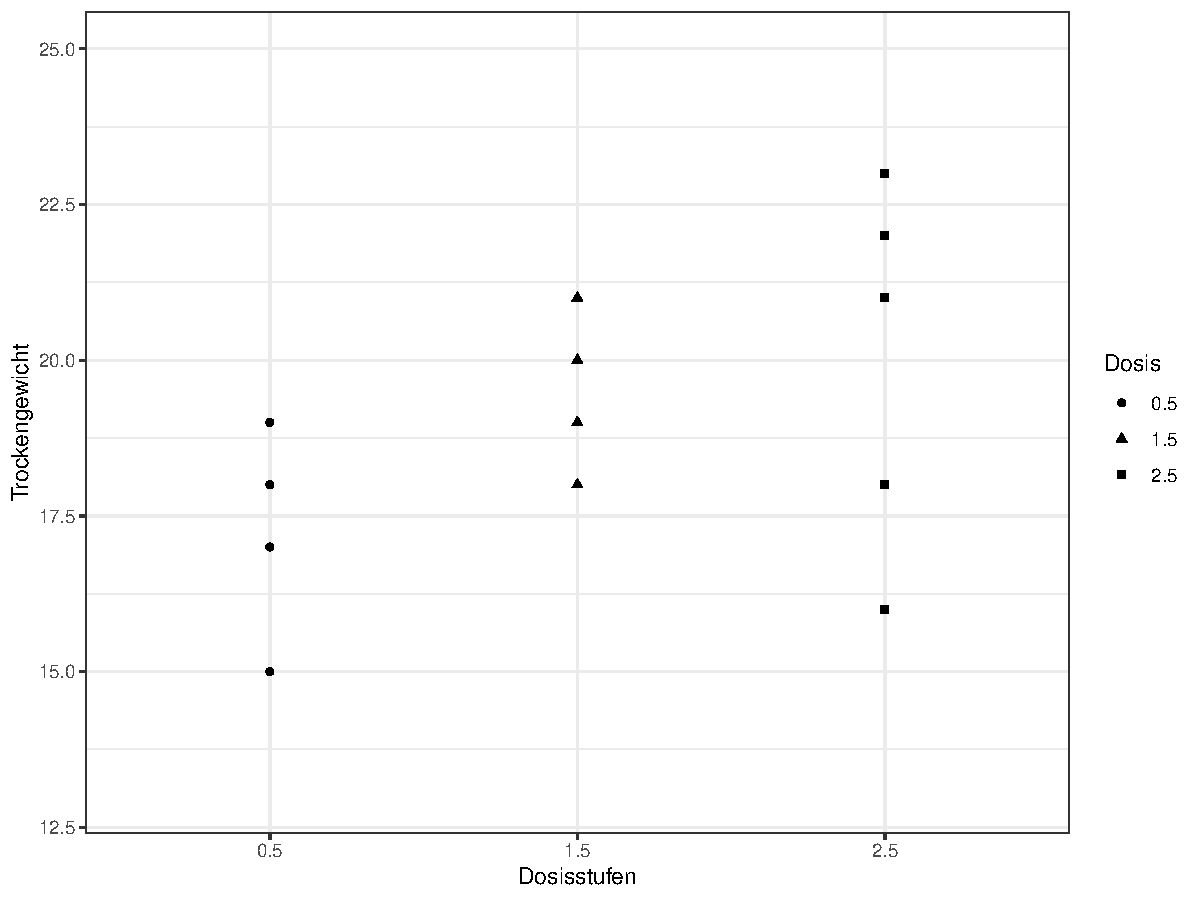
\includegraphics[width=\maxwidth]{img/anova-01-a-1} 

}


\end{knitrout}

\begin{enumerate}
\item Zeichnen Sie folgende statistischen Masszahlen in die Abildung ein!
  Beschriften Sie die statistischen Ma{\ss}zahlen! \textbf{(6 Punkte)}
  \begin{itemize}
  \item Total (grand) mean: $\beta_0$
  \item Mittelwerte der Dosen: $\bar{y}_{0.5}$, $\bar{y}_{1.5}$ und $\bar{y}_{2.5}$
  \item Effekt der einzelnen Level der Dosen: $\beta_{0.5}$, $\beta_{1.5}$,
    und $\beta_{2.5}$
  \item Residuen oder Fehler: $\epsilon$
  \end{itemize}
\item Liegt ein \textit{vermutlicher} signifikanter Unterschied zwischen
  den Dosisstufen vor? Begr{\"u}nden Sie Ihre Antwort! \textbf{(2 Punkte)}
\end{enumerate}
 
\clearpage
% -----------------------------------------------------------------------

\section{Aufgabe \hfill (13 Punkte)}

%% --------------------------------------------------------------------
\hfill\href{https://youtu.be/49hvImMwVyE}{
\includegraphics[width =
  2cm]{img/youtube}}\\[1Ex]
%% --------------------------------------------------------------------


Der Datensatz \texttt{plant\_growth\_tbl} enth{\"a}lt das Gewicht der Kohlk{\"o}pfe
(\textit{weight}), die unter einer Kontrolle und zwei verschiedenen
Behandlungsbedingungen erzielt wurden -- dem Faktor \textit{group} mit den
Faktorstufen \textit{ctrl}, \textit{trt1}, \textit{trt2}.



\begin{enumerate}
\item F{\"u}llen Sie die unterstehende einfaktorielle ANOVA Ergebnistabelle aus
  mit den gegebenen Informationen von \texttt{Df} und \texttt{Sum Sq}!
  \textbf{(4 Punkte)}
\item Sch{\"a}tzen Sie den p-Wert der Tabelle mit der Information von
  $F_{\alpha = 5\%} = 3.4$ ab. Begr{\"u}nden Sie Ihre
  Antwort! \textbf{(2 Punkte)}
\end{enumerate}

\vspace{1Ex}

\begin{center}
  \Large
  \begin{tabular}{l|c|c|c|c|c}
     & \textbf{Df} & \textbf{Sum Sq} & \textbf{Mean Sq} & \textbf{F value} & \textbf{Pr(>F)} \strut\\
    \hline
   \textbf{group}  & 2 & 29.85 &  &  &  \strut\\
    \hline
   \textbf{Residuals}  & 24 & 65.33 &  &  &  \strut\\
  \end{tabular}
\end{center}

\vspace{1Ex}

\begin{enumerate}
  \setcounter{enumi}{2}
\item Was bedeutet ein signifikantes Ergebnis in einer einfaktoriellen
  ANOVA im Bezug auf die m{\"o}glichen Unterschiede zwischen den Gruppen? Beziehen Sie sich auf den obigen Fragetext bei Ihrer Antwort!
  \textbf{(2 Punkte)}
\item Berechnen Sie \textit{einen} Student t-Test mit f{\"u}r den \textit{vermutlich}
  signifikantesten Gruppenvergleich anhand der untenstehenden Tabelle mit
  $T_{\alpha = 5\%} = 2.03$. Begr{\"u}nden Sie Ihre Auswahl! \textbf{(3 Punkte)}
\end{enumerate}

\begin{knitrout}
\definecolor{shadecolor}{rgb}{0.969, 0.969, 0.969}\color{fgcolor}\begin{table}[!h]
\centering
\begin{tabular}{cccc}
\toprule
group & n & mean & sd\\
\midrule
ctrl & 9 & 18.56 & 0.88\\
trt1 & 9 & 19.56 & 1.74\\
trt2 & 9 & 21.11 & 2.09\\
\bottomrule
\end{tabular}
\end{table}

\end{knitrout}

\begin{enumerate}
  \setcounter{enumi}{4}
\item Gegebenen der ANOVA Tabelle war das Ergebnis des t-Tests zu erwarten?
  Begr{\"u}nden Sie Ihre Antwort! \textbf{(2 Punkte)}
\end{enumerate}

 
\clearpage
% -----------------------------------------------------------------------

\section{Aufgabe \hfill (9 Punkte)}

%% --------------------------------------------------------------------
\hfill\href{https://youtu.be/d4CFR2MKX7I}{
\includegraphics[width =
  2cm]{img/youtube}}\\[1Ex]
%% --------------------------------------------------------------------

Der Datensatz \textit{crop\_tbl} enth{\"a}lt das Trockengewicht der
Maispflanzen (\textit{drymatter}), die unter drei 
verschiedenen D{\"u}ngerbedingungen erzielt wurden. Die D{\"u}ngerbedingungen sind in dem Faktor
\textit{trt} mit den Faktorstufen \textit{A},  \textit{trt1} und
 \textit{trt2} codiert. Sie erhalten folgenden Output in \Rlogo.

\begin{knitrout}
\definecolor{shadecolor}{rgb}{0.969, 0.969, 0.969}\color{fgcolor}\begin{kframe}
\begin{verbatim}
## Analysis of Variance Table
## 
## Response: drymatter
##           Df Sum Sq Mean Sq F value Pr(>F)
## trt        2 16.589  8.2946  2.4777  0.107
## Residuals 22 73.651  3.3478
\end{verbatim}
\end{kframe}
\end{knitrout}

\begin{enumerate}
\item Stellen Sie die statistische $H_0$ und $H_A$ Hypothese f{\"u}r die obige
  einfaktorielle ANOVA auf! \textbf{(2 Punkte)}
\item Interpretieren Sie das Ergebnis der einfaktoriellen ANOVA! \textbf{(2 Punkt)} 
\item Berechen Sie den Effektsch{\"a}tzer $\eta^2$. Was sagt Ihnen der Wert von
  $\eta^2$ aus? \textbf{(2 Punkte)}
\item Skizieren Sie eine Abbildung, der dem obigen Ergebnis der
  einfaktoriellen ANOVA n{\"a}herungsweise entspricht! \textbf{(3 Punkte)}
\end{enumerate}

 
\clearpage
% -----------------------------------------------------------------------

\section{Aufgabe \hfill (6 Punkte)}

%% --------------------------------------------------------------------
\hfill\href{https://youtu.be/zDK2dhgtFt0}{
\includegraphics[width =
  2cm]{img/youtube}}\\[1Ex]
%% --------------------------------------------------------------------


Sie haben ein Experiment mit drei Behandlungen (A, B und C) und vier
Bl{\"o}cken (I, II, III und IV) durchgef{\"u}hrt. Insgesamt haben Sie die Wuchsh{\"o}he
von zw{\"o}lf Sonnenblumen bestimmt. Im Folgenden sehen Sie die Wuchsh{\"o}hen in
[cm] aus dem Experiment.


\begin{knitrout}
\definecolor{shadecolor}{rgb}{0.969, 0.969, 0.969}\color{fgcolor}\begin{kframe}
\begin{verbatim}
##  [1] 111 111 119 107 105 109 140 131 146 148 141 134
\end{verbatim}
\end{kframe}
\end{knitrout}

Erstellen Sie vier Zeichnungen des experimentellen Designs und beachten
Sie folgende Angaben zu der Quelle der erkl{\"a}rten Varianz. 

\begin{enumerate}
\item Ordnen Sie die Pflanzen so in den vier Bl{\"o}cken und drei Behandlungen an,
  \begin{enumerate}
  \item[(1)] dass die Bl{\"o}cke \textit{kaum} Varianz erkl{\"a}ren. \textbf{(1 Punkt)}
  \item[(2)] dass die Bl{\"o}cke \textit{viel} Varianz erkl{\"a}ren. \textbf{(1 Punkt)}  
  \item[(3)] dass die Behandlungen \textit{kaum} Varianz erkl{\"a}ren. \textbf{(1 Punkt)}
  \item[(4)] dass die Behandlungen \textit{viel} Varianz erkl{\"a}ren. \textbf{(1 Punkt)}
  \end{enumerate}
\item Wenn Sie ein geplantes Experiment durchf{\"u}hren, wie viel Varianz soll dann von
  den Bl{\"o}cken und den Behandlungen jeweils erkl{\"a}rt werden? Begr{\"u}nden Sie
  Ihre Antwort! \textbf{(2 Punkte)}
\end{enumerate}
 
\clearpage
% -----------------------------------------------------------------------

\section{Aufgabe \hfill (12 Punkte)}

%% --------------------------------------------------------------------
\hfill\href{https://youtu.be/8Pb2sKUIMyk}{
\includegraphics[width =
  2cm]{img/youtube}}\\[1Ex]
%% --------------------------------------------------------------------



Der Datensatz \textit{tooth\_tbl} enth{\"a}lt Daten aus einer Studie zur
Bewertung der Wirkung von Vitamin C auf das Zahnwachstum bei
Meerschweinchen. Der Versuch wurde an verschiedenen Schweinen durchgef{\"u}hrt,
wobei jedes Tier eine von 4 Vitamin-C-Dosen \textit{dose}
{\"u}ber eine von 3 Verabreichungsmethoden \textit{supp}
erhielt. Die Zahnl{\"a}nge wurde als normalverteiltes Outcome gemessen.



\begin{enumerate}
\item F{\"u}llen Sie die unterstehende zweifaktorielle ANOVA Ergebnistabelle aus
  mit den gegebenen Informationen von \texttt{Df} und \texttt{Sum Sq}!
  \textbf{(4 Punkte)}
\item Sch{\"a}tzen Sie den p-Wert der Tabelle mit der Information von den
  kritischen F-Werten mit
  $F_{supp} = 4.03$ und
  $F_{dose} = 2.78$ sowie
  $F_{supp:dose} = 2.78$ ab. Begr{\"u}nden Sie Ihre
  Antwort! \textbf{(4 Punkte)}
\end{enumerate}

\vspace{1Ex}

\begin{center}
  \Large
  \begin{tabular}{l|c|c|c|c|c}
     & \textbf{Df} & \textbf{Sum Sq} & \textbf{Mean Sq} & \textbf{F value} & \textbf{Pr(>F)} \strut\\
    \hline
   \textbf{supp}  & 1 & 290.07 &  &  &  \strut\\
    \hline
    \textbf{dose}  & 3 & 422.31 &  &  &  \strut\\
    \hline
    \textbf{supp:dose}  & 3 & 44.12 &  &  &  \strut\\
    \hline
   \textbf{Residuals}  & 52 & 649.02 &  &  &  \strut\\
  \end{tabular}
\end{center}

\vspace{1Ex}

\begin{enumerate}
  \setcounter{enumi}{2}
\item Was bedeutet ein signifikantes Ergebnis in einer zweifaktoriellen
  ANOVA im Bezug auf die m{\"o}glichen Unterschiede zwischen den Gruppen?
  Beziehen Sie sich dabei einmal auf den Faktor \textit{supp} und einmal
  auf den Faktor \textit{dose}! \textbf{(2 Punkte)}
\item Was sagt der Term \textit{supp:dose} aus? Interpretieren Sie das
  Ergebnis des abgesch{\"a}tzten p-Wertes! \textbf{(2 Punkte)}
\end{enumerate}
 
\clearpage
% -----------------------------------------------------------------------

\section{Aufgabe \hfill (8 Punkte)}

%% --------------------------------------------------------------------
\hfill\href{https://youtu.be/rWTyHXXlYjY}{
\includegraphics[width =
  2cm]{img/youtube}}\\[1Ex]
%% --------------------------------------------------------------------


Der Datensatz \textit{pig\_gain\_weight\_tbl} enth{\"a}lt Daten aus einer Studie zur Bewertung
der Wirkung vom Vitamin Selen auf das Wachstum bei Mastschweinen. Der
Versuch wurde an 60 Mastschweinen durchgef{\"u}hrt, wobei
jedes Tier eine von drei Selen-Dosen $dose$ (0.5 ng/Tag, 1 ng/Tag und 5 ng/Tag)
{\"u}ber eine von zwei Verabreichungsmethoden $form$ erhielt (Wasser oder
Festnahrung). Sie erhalten folgenden Output in \Rlogo.

\begin{knitrout}
\definecolor{shadecolor}{rgb}{0.969, 0.969, 0.969}\color{fgcolor}\begin{kframe}
\begin{verbatim}
## Analysis of Variance Table
## 
## Response: gain
##           Df Sum Sq Mean Sq F value    Pr(>F)
## dose       2 488.26 244.128 23.9527 8.456e-06
## form       1  25.14  25.144  2.4670    0.1337
## dose:form  2   8.46   4.232  0.4152    0.6663
## Residuals 18 183.46  10.192
\end{verbatim}
\end{kframe}
\end{knitrout}

\begin{enumerate}
\item Stellen Sie die statistische $H_0$ und $H_A$ Hypothese f{\"u}r die obige
  zweifaktorielle ANOVA f{\"u}r den Faktor form
  auf! \textbf{(2 Punkte)}
\item Interpretieren Sie das Ergebnis der zweifaktoriellen ANOVA. Gehen Sie
  im besonderen auf den Term $dose:form$ ein! \textbf{(2 Punkte)}
\item Zeichnen Sie eine Abbildung, der dem obigen Ergebnis der
  zweifaktoriellen ANOVA n{\"a}herungsweise entspricht! \textbf{(4 Punkte)}
\end{enumerate}
 
\clearpage
% -----------------------------------------------------------------------

\section{Aufgabe \hfill (8 Punkte)}


%% --------------------------------------------------------------------
\hfill\href{https://youtu.be/FjjJXkFJfIY}{
\includegraphics[width =
  2cm]{img/youtube}}\\[1Ex]
%% --------------------------------------------------------------------


In der untenstehenden Tabelle ist die Formel f{\"u}r den F-Test aus der ANOVA
und die Formel f{\"u}r den Student t-Test dargestellt. In der ANOVA berechnen
Sie die F-Statistik $F_{calc}$ und in dem Student t-Test die T-Statistik
$T_{calc}$.

\begin{center}
  \begin{tabular}{cc}
    $F_{calc} = \cfrac{MS_{treatment}}{MS_{error}}$ & $T_{calc} = \cfrac{\bar{y}_1 - \bar{y}_2}{s_p \cdot \sqrt{2/n_g}}$\\
  \end{tabular}
\end{center}


\begin{enumerate}
\item Erkl{\"a}ren Sie den konzeptionellen Zusammenhang zwischen der $F_{calc}$
  Statistik und $T_{calc}$ Statistik! \textbf{(2 Punkte)}
\item Visualisieren Sie eine nicht signifikante $F_{calc}$ Statistik sowie
  eine signifikante $F_{calc}$ Statistik anhand von $MS_{treatment}$ und
  $MS_{error}$! Beschriften Sie die Abbildung! \textbf{(2 Punkte)}
\item Erkl{\"a}ren Sie an der Formel des F-Tests sowie an der Abbildung warum
  das Minimum der F-Statistik 0 ist! \textbf{(2 Punkte)}
\item Wenn die F-Statistik 0 ist, spricht dies eher f{\"u}r oder gegen die
  Nullhypothese? Begr{\"u}nden Sie Ihre Antwort! \textbf{(2 Punkte)}
\end{enumerate}

 
\clearpage
% -----------------------------------------------------------------------

\section{Aufgabe \hfill (6 Punkte)}

%% --------------------------------------------------------------------
\hfill\href{https://youtu.be/2qG1Dws0MJo}{
\includegraphics[width =
  2cm]{img/youtube}}\\[1Ex]
%% --------------------------------------------------------------------


Sie rechnen eine zweifaktorielle ANOVA und erhalten einen signifikanten
Interaktionseffekt zwischen den beiden Faktoren $f_1$ und $f_2$. Der Faktor
$f_1$ hat drei Level. Der Faktor $f_2$ hat dagegen nur zwei Level.




\begin{enumerate}
\item Visualisieren Sie in zwei getrennten Abbildungen eine
  schwache und eine mittelere Interaktion zwischen
  den Faktoren $f_1$ und $f_2$! \textbf{(2 Punkte)}
\item Erkl{\"a}ren Sie den Unterschied zwischen den beiden St{\"a}rken der Interaktion!
  \textbf{(2 Punkte)}
\item Wenn eine signifikante Interaktion in den Daten vorliegt, wie ist
  dann das weitere Vorgehen bei einem Posthoc-Test?
  \textbf{(2 Punkte)}
\end{enumerate}

 
\clearpage
% -----------------------------------------------------------------------

\section{Aufgabe \hfill (7 Punkte)}

%% --------------------------------------------------------------------
\hfill\href{https://youtu.be/M9Uhm67ndxM}{
\includegraphics[width =
  2cm]{img/youtube}}\\[1Ex]
%% --------------------------------------------------------------------




Sie rechnen eine einfaktorielle ANOVA mit einem Faktor $f_1$ mit
drei Leveln. Nachdem Sie die einfaktorielle ANOVA gerechnet
haben, erhalten Sie einen p-Wert von $0.078$ und eine F Statistik mit
$F_{calc} = 1.2$. Als Sie sich die Boxplots der Behandlungen anschauen,
stellen Sie fest, dass es eigentlich einen Mittelwertsunterschied zwischen
dem dritten und zweiten Level geben m{\"u}sste. Die
$IQR$-Bereiche {\"u}berlappen sich nicht und die Mediane liegen auch weit vom
globalen Mittel entfernt.


\begin{enumerate}
\item Erkl{\"a}ren Sie die Annahme der Normalverteilung und die Annahme der
  Varianzhomogenit{\"a}t f{\"u}r eine ANOVA an einer passenden Abbildung! \textbf{(2 Punkte)}
\item Visualisieren Sie die Berechnung von $F_{calc}$ am obigen Beispiel!
  \textbf{(2 Punkte)}
\item Erkl{\"a}ren Sie das Ergebnis der obigen einfaktoriellen ANOVA unter der
  Ber{\"u}cksichtigung der Annahmen an eine ANOVA! \textbf{(3 Punkte)}
\end{enumerate}

 
\clearpage
% -----------------------------------------------------------------------
  \begin{graybox}{Der $\mathcal{X}^2$-Test \& Der diagnostische Test}
Mehr Informationen zu den Aufgaben in den folgenden Kapiteln aus dem Skript Bio Data Science.
  \begin{itemize}
  \item \href{https://jkruppa.github.io/stat-tests-chi-test.html}{Kapitel 28 - Der $\mathcal{X}^2$-Test}
  \item \href{https://jkruppa.github.io/stat-tests-diagnostic.html}{Kapitel 29 - Der diagnostische Test}
  \end{itemize}
\end{graybox}
\clearpage
% -----------------------------------------------------------------------

\section{Aufgabe \hfill (10 Punkte)}

%% --------------------------------------------------------------------
\hfill\href{https://youtu.be/PVUK0zdkZkk}{
\includegraphics[width =
  2cm]{img/youtube}}\\[1Ex]
%% --------------------------------------------------------------------




Nach einem Experiment ergibt sich die folgende 2x2 Datentabelle mit einem
Pestizid (ja/nein), dargestellt in den Zeilen. Im Weiteren mit dem
infizierten Pflanzenstatus (ja/nein) in den Spalten. Insgesamt wurden
$n = 142$ Pflanzen untersucht.
\vspace{5Ex}

\begin{center}
  \Large
  \begin{tabular}{c|c|c|c}
     & \textbf{Erkrankt (ja)} & \textbf{Erkrankt (nein)} &  \strut\\
    \hline
    \textbf{Pestizid (ja)} & 56  & 19  &     \strut\\
    \hline
    \textbf{Pestizid (nein)} & 23  & 44  &      \strut\\
    \hline
     \phantom{100} & \phantom{100}  & \phantom{100}  &  \phantom{100}  \strut\\
  \end{tabular}
\end{center}

\vspace{5Ex}

\begin{enumerate}
\item Erg{\"a}nzen Sie die Tabelle um die Randsummen! \textbf{(1 Punkt)} 
\item Formulieren Sie die Fragestellung! \textbf{(1 Punkt)}
\item Formulieren Sie das Hypothesenpaar! \textbf{(2 Punkte)}
\item Berechnen Sie die Teststatistik eines Chi-Quadrat-Test auf der 2x2
  Tafel. Geben Sie Formeln und Rechenweg mit an! \textbf{(4 Punkte)}
\item Treffen Sie eine Entscheidung im Bezug zu der Nullhypothese gegeben
  einem $\mathcal{X}^2_{\alpha = 5\%} = 3.841$! \textbf{(1 Punkt)}
\item Skizzieren Sie eine 2x2 Tabelle mit
  $n = 26$ Pflanzen in dem \textit{vermutlich}
  die Nullhypothese nicht abgelehnt werden kann! \textbf{(1 Punkt)}
\end{enumerate} 
\clearpage
% -----------------------------------------------------------------------

\section{Aufgabe \hfill (7 Punkte)}

%% --------------------------------------------------------------------
\hfill\href{https://youtu.be/jakM7fHyZfU}{\includegraphics[width =
  2cm]{img/youtube}}\\[1Ex]
%% --------------------------------------------------------------------




Gegeben sind folgende Randsummen in einer 2x2 Kreuztabelle aus einem
Experiment mit $n = 124$ Sauen. In dem Experiment wurde gemessen,
ob eine Sau nach einer Behandlung mit einem Medikament (ja/nein)
mehr als 30 Ferkel pro Jahr bekommen konnte (ja/nein).

\vspace{5Ex}

\begin{center}
  \Large
  \begin{tabular}{c|c|c|c}
     & \textbf{>30 Ferkel (ja)} & \textbf{$\leq$30 Ferkel (nein)} &  \strut\\
    \hline
    \textbf{Medikament (ja)} & \phantom{100}  & \phantom{100}  &   63  \strut\\
    \hline
    \textbf{Medikament (nein)} & \phantom{100}  & \phantom{100}  &   61   \strut\\
    \hline
     &  74 &  50 &  124  \strut\\
  \end{tabular}
\end{center}



\vspace{5Ex}

\begin{enumerate}
\item Erg{\"a}nzen Sie die Felder innerhalb der 2x2 Kreuztabelle in dem Sinne,
  dass \textit{ein} signifikanter Effekt zu erwarten w{\"a}re!
  \textbf{(2 Punkte)}
\item Erkl{\"a}ren und Begr{\"u}nden Sie Ihr Vorgehen an der Formel des
  Chi-Quadrat-Tests mit
  \begin{equation*}
  \mathcal{X}^2 = \sum\tfrac{(O - E)^2}{E}.  
  \end{equation*}
  Sie k{\"o}nnen dies an einem Beispiel erkl{\"a}ren! \textbf{(2 Punkte)}
\item Was ist die Mindestanzahl an Beobachtungen je Zelle? Wenn in einer
  der Zellen weniger Beobachtungen auftreten, welchen Test k{\"o}nnen Sie
  anstatt des "`normalen"' Chi-Quadrat-Tests anwenden? \textbf{(2 Punkte)}
\item Warum hat die obige Vierfeldertafel einen Freiheitsgrad von $df=1$?
  \textbf{(1 Punkt)}
\end{enumerate} 
\clearpage
% -----------------------------------------------------------------------

\section{Aufgabe \hfill (11 Punkte)}

%% --------------------------------------------------------------------
\hfill\href{https://youtu.be/VQlNl8hvRII}{\includegraphics[width =
  2cm]{img/youtube}}\\[1Ex]
%% --------------------------------------------------------------------


Die Pr{\"a}valenz von Klauenseuche bei Wollschweinen wird mit
4\% angenommen. In 75\% der F{\"a}lle ist ein Test positiv, wenn das Wollschwein erkrankt
ist. In 8\% der F{\"a}lle ist ein Test positiv,
wenn das Wollschwein \textit{nicht} erkrankt ist und somit gesund ist. Sie
werten 1000 Wollschweine mit einem
diagnostischen Test auf Klauenseuche aus.



\begin{enumerate}
\item F{\"u}llen und beschriften Sie den untenstehenden Doppelbaum! Beschriften
  Sie auch die {\"A}ste des Doppelbaumes, mit denen Ihnen bekannten
  Informationen!  \textbf{(8 Punkte)}
\item Berechnen Sie die Wahrscheinlichkeit $Pr(K^+|T^+)$! \textbf{(2 Punkte)}
\item Was sagt Ihnen die Wahrscheinlichkeit $Pr(K^+|T^+)$ aus? \textbf{(1 Punkt)}
\end{enumerate}

\vspace{1cm}

\begin{center}
  \includegraphics[width=17cm]{/Users/kruppajo/Documents/GitHub/exam/question/img/diag-doppelbaum}
\end{center}



 
\clearpage
% -----------------------------------------------------------------------

\section{Aufgabe \hfill (12 Punkte)}


%% --------------------------------------------------------------------
\hfill\href{https://youtu.be/_7s44pbOc00}{\includegraphics[width =
  2cm]{img/youtube}}\\[1Ex]
%% --------------------------------------------------------------------





Folgender diagnostischer Doppelbaum nach der Testung auf Klauenseuche bei
Fleckvieh ist gegeben.

\begin{enumerate}
\item F{\"u}llen und beschriften Sie den untenstehenden Doppelbaum! \textbf{(4
    Punkte)}
\item Berechnen Sie die Wahrscheinlichkeit $Pr(K^+|T^+)$! \textbf{(2 Punkte)}
\item Berechnen Sie die Pr{\"a}valenz f{\"u}r Klauenseuche! \textbf{(2 Punkte)}
\item Berechnen Sie die Sensifit{\"a}t und Spezifit{\"a}t des diagnostischen Tests
  f{\"u}r Klauenseuche! Erstellen Sie daf{\"u}r zun{\"a}chst eine 2x2 Kreuztabelle aus
  dem ausgef{\"u}llten Doppelbaum!
  \textbf{(4 Punkte)}
\end{enumerate}

\vspace{1cm}
 
\begin{tikzpicture}
  \node (image) at (0,0) {
    \includegraphics[width=\textwidth]{/Users/kruppajo/Documents/GitHub/exam/question/img/diag-doppelbaum}
  };
  \node[] at (-4.8,0) {\huge 180};
  \node[] at (-1.7,0) {\huge 40};
  \node[] at (1.7,0) {\huge 850};
  \node[] at (4.75,0) {\huge 1600};
\end{tikzpicture}




 
\clearpage
% -----------------------------------------------------------------------

\section{Aufgabe \hfill (10 Punkte)}

%% --------------------------------------------------------------------
\hfill\href{https://youtu.be/G-_r2KplGTI}{\includegraphics[width =
  2cm]{img/youtube}}\\[1Ex]
%% --------------------------------------------------------------------


Beim diagnostischen Testen erhalten Sie \textit{True Positives (TP)},
\textit{True Negatives (TN)}, \textit{False Positives (FP)} und
\textit{False Negatives (FN)}. Erkl{\"a}ren Sie den Zusammenhang wir folgt.

\begin{enumerate}
\item Tragen Sie \textit{TP}, \textit{TN}, \textit{FP} und \textit{FN} in
  eine 2x2 Kreuztablle ein. Beschriften Sie die Tabelle entsprechend!
  \textbf{(2 Punkte)}
\item Visualisieren Sie \textit{TP}, \textit{TN}, \textit{FP} und
  \textit{FN} in einer Abbildung. Beschriften Sie die Abbildung und die
  Achsen entsprechend! \textbf{(4 Punkte)}
\item Erkl{\"a}ren Sie an einem numerischen Beispiel und der Abbildung die
  Berechnung der Pr{\"a}valenz!  \textbf{(2 Punkte)}
\item Erkl{\"a}ren Sie an einem Schaubild den Unterschied zwischen Inzidenz und
  Pr{\"a}valenz!  \textbf{(2 Punkte)}
\end{enumerate}





 
\clearpage
% -----------------------------------------------------------------------
\begin{graybox}{Simple lineare Regression}
Mehr Informationen zu den Aufgaben in den folgenden Kapiteln aus dem Skript Bio Data Science.
  \begin{itemize}
  \item \href{https://jkruppa.github.io/stat-linear-reg-basic.html}{Kapitel 32 - Simple lineare Regression}
  \item \href{https://jkruppa.github.io/stat-linear-reg-quality.html}{Kapitel 33 - Maßzahlen der Modelgüte}
  \item \href{https://jkruppa.github.io/stat-linear-reg-corr.html}{Kapitel 34 - Korrelation}
  \end{itemize}
\end{graybox}
\clearpage
% -----------------------------------------------------------------------

\section{Aufgabe \hfill (7 Punkte)}

%% --------------------------------------------------------------------
\hfill\href{https://youtu.be/2dUJcYK9RgU}{\includegraphics[width =
  2cm]{img/youtube}}\\[1Ex]
%% --------------------------------------------------------------------

In einer Studie zur "`Arbeitssicherheit auf dem Feld"' wurde gemessen wie viele
Stunden auf einem Feld gefahren wurden und wie oft der Fahrer dabei drohte
einzunicken. Es ergab sich folgende Abbildung. 



{\centering \includegraphics[width=\maxwidth]{img/scatter-02-1} 

}




\begin{enumerate}
\item Erstellen Sie die Regressionsgleichung aus der obigen Abbildung in
  der Form $y \sim \beta_0 + \beta_1 \cdot x$! \textbf{(2 Punkte)}
\item Beschriften Sie die Gerade mit den Parametern der linearen
  Regressionsgleichung! \textbf{(2 Punkte)}
\item Liegt ein Zusammenhang zwischen der Anzahl an gefahrenen Runden und
  der M{\"u}digkeit vor? Begr{\"u}nden Sie Ihre Antwort! \textbf{(2 Punkte)}
\item Wenn kein Zusammenhang zu beobachten w{\"a}re, wie w{\"u}rde die Gerade aussehen? \textbf{(1 Punkt)}
\end{enumerate} 
\clearpage
% -----------------------------------------------------------------------

\section{Aufgabe \hfill (10 Punkte)}

%% --------------------------------------------------------------------
\hfill\href{https://youtu.be/lJp8rFmMnrs}{\includegraphics[width =
  2cm]{img/youtube}}\\[1Ex]
%% --------------------------------------------------------------------



In einem Stallexperiment mit $n = 40$ Ferkeln wurde der
Gewichtszuwachs unter bestimmten Lichtverh{\"a}ltnissen gemessen. Sie erhalten
den \Rlogo Output der Funktion \texttt{tidy()} einer simplen Gaussian linearen
Regression sieben Wochen nach der ersten Messung.

\begin{table}[!h]
\centering\begingroup\fontsize{14}{16}\selectfont

\begin{tabular}{ccccc}
\toprule
term & estimate & std.error & t statistic & p-value\\
\midrule
(Intercept) & 22.08 & 2.33 &  & \\
light & 1.28 & 0.24 &  & \\
\bottomrule
\end{tabular}
\endgroup{}
\end{table}



\begin{enumerate}
\item Berechnen Sie die t Statistik f{\"u}r \textit{(Intercept)} und
  \textit{light}! \textbf{(2 Punkte)}
\item Sch{\"a}tzen Sie den p-Wert f{\"u}r \textit{(Intercept)} und
  \textit{light} mit $T_{\alpha = 5\%} = 1.96$ ab. Was sagt Ihnen der p-Wert aus?
  Begr{\"u}nden Sie Ihre Antwort! \textbf{(3 Punkte)}
\item Zeichnen Sie die Gerade aus der obigen Tabelle in ein Koordinatenkreuz! \textbf{(1 Punkt)}
\item Beschriften Sie die Abbildung und die Gerade mit den statistischen
  Kenngr{\"o}{\ss}en! \textbf{(2 Punkte)}
\item Formulieren Sie die Regressionsgleichung! \textbf{(2 Punkte)}
\end{enumerate} 
\clearpage
% -----------------------------------------------------------------------

\section{Aufgabe \hfill (6 Punkte)}

%% --------------------------------------------------------------------
\hfill\href{https://youtu.be/tNNzcndrpSk}{\includegraphics[width =
  2cm]{img/youtube}}\\[1Ex]
%% --------------------------------------------------------------------

Sie erhalten folgende R Ausgabe der Funktion lm() nach einem Experiment mit
zwei Behandlungen (A und B) sowie dem Ertragsgewicht von Weizen.

\begin{knitrout}
\definecolor{shadecolor}{rgb}{0.969, 0.969, 0.969}\color{fgcolor}\begin{kframe}
\begin{verbatim}
## 
## Call:
## lm(formula = weight ~ trt, data = data_tbl)
## 
## Residuals:
##     Min      1Q  Median      3Q     Max 
## -3.6000 -1.8286 -0.5857  2.4071  4.4286 
## 
## Coefficients:
##             Estimate Std. Error t value Pr(>|t|)
## (Intercept)   18.600      1.334  13.948 7.02e-08
## trtB          -4.029      1.746  -2.307   0.0437
## 
## Residual standard error: 2.982 on 10 degrees of freedom
## Multiple R-squared:  0.3474,	Adjusted R-squared:  0.2822 
## F-statistic: 5.324 on 1 and 10 DF,  p-value: 0.04371
\end{verbatim}
\end{kframe}
\end{knitrout}


\begin{enumerate}
\item Ist die Annahme der Normalverteilung an das Outcome \textit{rsp} erf{\"u}llt?
  Begr{\"u}nden Sie die Antwort! \textbf{(2 Punkte)}
\item Wie gro{\ss} ist der Effekt des \textit{Trt}? Liegt ein signifikanter
  Effekt vor? Begr{\"u}nden Sie Ihre Antwort! \textbf{(2 Punkte)}
\item Schreiben Sie das Ergebnis der \Rlogo Ausgabe in einen Satz nieder, der die
  Information zum Effekt und der Signifikanz enth{\"a}lt! \textbf{(2 Punkte)} 
\end{enumerate}
 
\clearpage
% -----------------------------------------------------------------------

\section{Aufgabe \hfill (8 Punkte)}

%% --------------------------------------------------------------------
\hfill\href{https://youtu.be/C_a8aOMI7GE}{\includegraphics[width =
  2cm]{img/youtube}}\\[1Ex]
%% --------------------------------------------------------------------



\begin{enumerate}
\item Skizieren Sie in die unten stehenden, freien Abbildungen ein kausales
  und ein pr{\"a}diktives Modell mit $n = 5$
  Beobachtungen! \textbf{(4 Punkte)}
\item Beachten Sie bei der Erstellung der Skizze, ob ein Effekt von X
  vorliegt oder nicht! \textbf{(2 Punkte)}
\item Beschriften Sie die Abbildung mit "`Trainingsdaten"' und "`Testdaten"'!  \textbf{(2 Punkte)}
\end{enumerate}



{\centering \includegraphics[width=\maxwidth]{img/modeling-01-1} 

}



 
\clearpage
% -----------------------------------------------------------------------

\section{Aufgabe \hfill (9 Punkte)}

%% --------------------------------------------------------------------
\hfill\href{https://youtu.be/fB6nF4dxodA}{\includegraphics[width =
  2cm]{img/youtube}}\\[1Ex]
%% --------------------------------------------------------------------


Im folgenden sehen Sie drei leere Scatterplots. F{\"u}llen Sie diese
Scatterplots nach folgenden Anweisungen.

\begin{enumerate}
\item Zeichnen Sie f{\"u}r die angegebene $\rho$-Werte eine Gerade in die
  entsprechende Abbildung! \textbf{(3 Punkte)}
\item Zeichnen Sie f{\"u}r die angegebenen $R^2$-Werte die entsprechende
  Punktewolke um die Gerade. \textbf{(3 Punkte)}
\item Sie rechnen ein statistisches Modell. Was sagen Ihnen die $R^2$-Werte
  {\"u}ber das jeweilige Modell? \textbf{(3 Punkte)}
\end{enumerate}




{\centering \includegraphics[width=\maxwidth]{img/correlation-01-1} 

}



 
\clearpage
% -----------------------------------------------------------------------

\section{Aufgabe \hfill (9 Punkte)}

%% --------------------------------------------------------------------
\hfill\href{https://youtu.be/2QJa19ZwLls}{\includegraphics[width =
  2cm]{img/youtube}}\\[1Ex]
%% --------------------------------------------------------------------

Im folgenden sehen Sie vier Scatterplots. Erg{\"a}nzen Sie die {\"U}berschriften
der jeweiligen Scatterplots.


\begin{enumerate}
\item Sch{\"a}tzen Sie die $\rho$-Werte in der entsprechenden
  Abbildung! \textbf{(4 Punkte)}
\item Sch{\"a}tzen Sie die $R^2$-Werte in der entsprechenden
  Punktewolke um die Gerade! \textbf{(4 Punkte)}
\item Sie rechnen ein statistisches Modell. Was sagen Ihnen die $R^2$-Werte
  {\"u}ber das jeweilige Modell? \textbf{(1 Punkt)}
\end{enumerate}




{\centering \includegraphics[width=\maxwidth]{img/correlation-02-1} 

}



 
\clearpage
% -----------------------------------------------------------------------

\section{Aufgabe \hfill (12 Punkte)}

%% --------------------------------------------------------------------
\hfill\href{https://youtu.be/C9skfFRTHhI}{\includegraphics[width =
   2cm]{img/youtube}}\\[1Ex]
%% --------------------------------------------------------------------

Sie erhalten folgende \Rlogo Ausgabe der Funktion \texttt{cor.test()}.

\begin{knitrout}
\definecolor{shadecolor}{rgb}{0.969, 0.969, 0.969}\color{fgcolor}\begin{kframe}
\begin{verbatim}
## 
## 	Spearman's correlation
## 
## data:  height and food
## t = 1.7094, df = 8, p-value = 0.1258
## alternative hypothesis: true correlation is not equal to 0
## 95 percent confidence interval:
##  -0.1666774  0.8651197
## sample estimates:
##       cor 
## 0.5172292
\end{verbatim}
\end{kframe}
\end{knitrout}


\begin{enumerate}
  \item Formulieren Sie das statistische Hypothesenpaar! \textbf{(1
Punkt)}
\item Nennen Sie die zwei Eigenschaften des Korrelationskoeffizienten!
  Erkl{\"a}ren Sie \textit{eine} der Eigenschaften an einem Beispiel! \textbf{(3
    Punkte)}
\item Sind die Variablen \texttt{height and food} normalverteilt?
  Begr{\"u}nden Sie Ihre Antwort! \textbf{(2 Punkte)}
\item Interpretieren Sie den Korrelationskoefizienten hinsichtlich des
  Effekts und der Signifikanz! Begr{\"u}nden Sie
  Ihre Antwort! \textbf{(3 Punkte)}
\item Visualisieren Sie die Teststatistik und den p-Wert! Beschriften Sie die Abbildung! \textbf{(3 Punkte)} 
\end{enumerate} 
\clearpage
% -----------------------------------------------------------------------

\section{Aufgabe \hfill (6 Punkte)}

%% --------------------------------------------------------------------
\hfill\href{https://youtu.be/EK7JEtdZbnw}{\includegraphics[width =
  2cm]{img/youtube}}\\[1Ex]
%% --------------------------------------------------------------------




\begin{enumerate}
\item Skizieren Sie in die unten stehenden, freien Abbildungen die
  Abbildung, die sich nach der {\"U}berschrift ergibt! \textbf{(4 Punkte)}
\item Beschriften Sie die Achsen entsprechend! \textbf{(2 Punkte)}
\end{enumerate}



{\centering \includegraphics[width=\maxwidth]{img/regression-03-1} 

}



 
\clearpage
% -----------------------------------------------------------------------

\section{Aufgabe \hfill (7 Punkte)}

%% --------------------------------------------------------------------
\hfill\href{https://youtu.be/cYyvOXR4qa8}{\includegraphics[width =
  2cm]{img/youtube}}\\[1Ex]
%% --------------------------------------------------------------------




\begin{enumerate}
\item Skizieren Sie in die unten stehenden, freien Abbildungen die
  Abbildung, die sich nach der {\"U}berschrift ergibt! \textbf{(4 Punkte)}
\item Beschriften Sie die Achsen entsprechend! \textbf{(3 Punkte)}
\end{enumerate}



{\centering \includegraphics[width=\maxwidth]{img/regression-04-1} 

}



 
\clearpage
% -----------------------------------------------------------------------

\section{Aufgabe \hfill (10 Punkte)}

%% --------------------------------------------------------------------
\hfill\href{https://youtu.be/dyQlYV9nOqY}{\includegraphics[width =
  2cm]{img/youtube}}\\[1Ex]
%% --------------------------------------------------------------------

Sie rechnen eine lineare Regression um nach einem Feldexperiment den
Zusammenhang zwischen Trockengewicht kg/m$^2$ (\textit{drymatter}) und
Wassergabe l/m$^2$ (\textit{water}) bei Spargel zu bestimmen. Sie erhalten
folgende Datentabelle.

\begin{knitrout}
\definecolor{shadecolor}{rgb}{0.969, 0.969, 0.969}\color{fgcolor}\begin{table}[!h]
\centering\begingroup\fontsize{12}{14}\selectfont

\begin{tabular}{ccccc}
\toprule
.id & drymatter & water & .fitted & .resid\\
\midrule
1 & 30.4 & 12.5 & 29.1 & \\
2 & 33.4 & 11.7 & 27.8 & \\
3 & 33.1 & 15.0 & 32.8 & \\
4 & 17.8 & 5.2 & 18.4 & \\
5 & 33.8 & 16.4 & 34.9 & \\
\addlinespace
6 & 23.5 & 11.0 & 26.8 & \\
7 & 40.1 & 20.8 & 41.3 & \\
8 & 20.7 & 6.9 & 20.9 & \\
9 & 15.9 & 4.1 & 16.8 & \\
\bottomrule
\end{tabular}
\endgroup{}
\end{table}

\end{knitrout}

\begin{enumerate}
\item Erg{\"a}nzen Sie die Werte in der Spalte \texttt{.resid} in der obigen
  Tabelle. Geben Sie den Rechenweg und Formel mit an! \textbf{(4 Punkte)}
\item Zeichnen Sie den sich aus der obigen Tabelle ergebenden
  Residualplot. Beschriften Sie die Abbildung! \textbf{(4 Punkte)}
\item Gibt es auff{\"a}llige Werte anhand des Residualplots? Begr{\"u}nden Sie Ihre
  Antwort! \textbf{(2 Punkte)}
\end{enumerate}
 
\clearpage
% -----------------------------------------------------------------------
\begin{graybox}{Multiple lineare Regression}
Mehr Informationen zu den Aufgaben in den folgenden Kapiteln aus dem Skript Bio Data Science.
  \begin{itemize}
  \item \href{https://jkruppa.github.io/stat-modeling-basic.html}{Kapitel 35 - Multiple lineare Regression}
  \item \href{https://jkruppa.github.io/stat-modeling-gaussian.html}{Kapitel 40 - Gaussian Regression}
  \item \href{https://jkruppa.github.io/stat-modeling-poisson.html}{Kapitel 41 - Poisson Regression}
  \item \href{https://jkruppa.github.io/stat-modeling-logistic.html}{Kapitel 43 - Logistische Regression}
  \item \href{https://jkruppa.github.io/stat-modeling-mixed.html}{Kapitel 44 - Lineare gemischte Modelle}
  \end{itemize}
\end{graybox}
\clearpage
% -----------------------------------------------------------------------

\section{Aufgabe \hfill (12 Punkte)}

%% --------------------------------------------------------------------
\hfill\href{https://youtu.be/lHzRgm7hPw0}{\includegraphics[width =
  2cm]{img/youtube}}\\[1Ex]
%% --------------------------------------------------------------------



\begin{enumerate}
\item Zeichen Sie in die drei untenstehenden, leeren Abbilungen die Zeile des
  Regressionskreuzes der Normalverteilung. W{\"a}hlen Sie die Beschriftung der
  y-Achse sowie der x-Achse entsprechend aus! \textbf{(6 Punkte)}
\item Erg{\"a}nzen Sie die jeweiligen statistischen Methoden zu der Abbildung! \textbf{(2 Punkte)}
\item Welchen Effektsch{\"a}tzer erhalten Sie aus der entsprechend linearen
  Regression bzw. den Gruppenvergleich? Geben Sie ein Beispiel! \textbf{(2 Punkte)}
\item Wenn Sie keinen Effekt erwarten, welchen \textit{Zahlenraum} nimmt dann
  der Effektsch{\"a}tzer ein? Geben Sie ein Beispiel! \textbf{(2 Punkte)}
\end{enumerate}



{\centering \includegraphics[width=\maxwidth]{img/regression-01-1} 

}



 
\clearpage
% -----------------------------------------------------------------------

\section{Aufgabe \hfill (9 Punkte)}

%% --------------------------------------------------------------------
\hfill\href{https://youtu.be/AwQEcQWLFCw}{\includegraphics[width =
  2cm]{img/youtube}}\\[1Ex]
%% --------------------------------------------------------------------



Ein Feldexperiment wurde mit $n = 200$ Pflanzen durchgef{\"u}hrt. Folgende
Einflussvariablen ($x$) wurden erhoben: region, height und dry. Als m{\"o}gliche Outcomevariablen stehen Ihnen nun
folgende gemessene Endpunkte zu Verf{\"u}gung: drymatter, yield, count, quality\_score und dead.

\begin{enumerate}
\item W{\"a}hlen Sie ein Outcome was zu der Verteilungsfamilie
  \textit{Gaussian} geh{\"o}rt! \textbf{(1 Punkt)}
\item Schreiben Sie das Modell in der Form $y \sim x$ wie es in \Rlogo in
  der Funktion \texttt{glm()}
  {\"u}blich ist \textit{ohne Interaktionsterm}! \textbf{(3 Punkte)}
\item Schreiben Sie das Modell in der Form $y \sim x$ wie es in \Rlogo
  {\"u}blich ist und erg{\"a}nzen Sie \textit{einen} Interaktionsterm nach Wahl! \textbf{(1 Punkt)} 
\item Zeichen Sie eine \textit{starke}
  Interaktion in die Abbildung unten f{\"u}r den Endpunkt
  \textit{yield}. Erg{\"a}nzen Sie eine aussagekr{\"a}ftige Legende. Wie erkennen
  Sie eine Interaktion? Begr{\"u}nden Sie Ihre Antwort! \textbf{(4 Punkte)}
\end{enumerate}



{\centering \includegraphics[width=\maxwidth]{img/modeling-R-01-1} 

}


 
\clearpage
% -----------------------------------------------------------------------

\section{Aufgabe \hfill (9 Punkte)}

%% --------------------------------------------------------------------
\hfill\href{https://youtu.be/NSMrpAYzOcs}{\includegraphics[width =
  2cm]{img/youtube}}\\[1Ex]
%% --------------------------------------------------------------------



Maispflanzen sollen auf die ertragssteigerende Wirkung von verschiedenen
Einflussfaktoren untersucht werden. Gemessen wurde als Outcome die
Trockenmasse in kg/m$^2$. Daf{\"u}r wurde f{\"u}r jede Maispflanze gemessen wieviel
Wasser (l/m$^2$) die Pflanze erhalten hat oder ob die Pflanze ein
neuartiges Lichtregime (0 = alt, 1 = neu) erhalten hatte. Zus{\"a}tzlich wurde
die Anzahl an Nematoden im Boden bestimmt sowie der Eisen- und
Phosphorgehalt ($\mu$g/kg) des Bodens. Es ergibt sich folgender Auszug aus
den Daten.

\begin{knitrout}
\definecolor{shadecolor}{rgb}{0.969, 0.969, 0.969}\color{fgcolor}\begin{table}[!h]
\centering
\begin{tabular}{lrrrrr}
\toprule
water & light & P & Fe & drymatter & nematodes\\
\midrule
10.43 & 0 & 9.40 & 102.03 & 73.30 & 7\\
8.60 & 0 & 12.21 & 102.94 & 69.92 & 10\\
10.51 & 0 & 10.07 & 101.92 & 71.88 & 12\\
10.18 & 0 & 9.82 & 102.02 & 72.66 & 8\\
\bottomrule
\end{tabular}
\end{table}

\end{knitrout}

Sie rechnen nun eine Gaussian lineare Regression auf den Daten und erhalten
folgenden \Rlogo Output.

{\small
\begin{knitrout}
\definecolor{shadecolor}{rgb}{0.969, 0.969, 0.969}\color{fgcolor}\begin{kframe}
\begin{verbatim}
## 
## Call:
## lm(formula = reformulate(response = "drymatter", termlabels = wanted_vec), 
##     data = data_tbl)
## 
## Residuals:
##     Min      1Q  Median      3Q     Max 
## -6.6180 -1.6186  0.1147  1.6270  6.0515 
## 
## Coefficients:
##             Estimate Std. Error t value Pr(>|t|)
## (Intercept)  0.14720    8.07515   0.018   0.9855
## water       -0.08613    0.14792  -0.582   0.5616
## light        1.18437    0.48965   2.419   0.0173
## Fe           0.70371    0.07797   9.025 1.01e-14
## 
## Residual standard error: 2.329 on 104 degrees of freedom
## Multiple R-squared:  0.4782,	Adjusted R-squared:  0.4632 
## F-statistic: 31.77 on 3 and 104 DF,  p-value: 1.165e-14
\end{verbatim}
\end{kframe}
\end{knitrout}
}


\begin{enumerate}
\item Sind die Residuals approximativ Normalverteilt? Begr{\"u}nden Sie Ihre Antwort! \textbf{(3 Punkte)}  
\item Welche der Einflussfaktoren sind signifikant? Begr{\"u}nden Sie Ihre
  Antwort! \textbf{(3 Punkte)}
\item Interpretieren Sie die Spalte \textit{estimate} im Bezug auf den
  Ertrag in Trockenmasse der Maispflanzen! \textbf{(3 Punkte)}
\end{enumerate}
 
\clearpage
% -----------------------------------------------------------------------

\section{Aufgabe \hfill (10 Punkte)}

%% --------------------------------------------------------------------
\hfill\href{https://youtu.be/K_28Ne6ladI}{\includegraphics[width =
  2cm]{img/youtube}}\\[1Ex]
%% --------------------------------------------------------------------




In verschiedenen Fl{\"u}{\ss}en (\textit{stream}) wurde die Anzahl an
Knochenhechten (\textit{longnose}) gez{\"a}hlt. Daneben wurden noch andere
Eigenschaften der entspechenden Fl{\"u}sse gemessen. Es ergibt sich folgender
Auszug aus den Daten. 


\begin{knitrout}
\definecolor{shadecolor}{rgb}{0.969, 0.969, 0.969}\color{fgcolor}\begin{table}[!h]
\centering
\begin{tabular}{lrrrrr}
\toprule
stream & longnose & no3 & so4 & temp & maxdepth\\
\midrule
BENNETT\_CR & 2 & 2.26 & 8.81 & 12.9 & 51\\
MUDLICK\_RUN & 8 & 0.84 & 16.30 & 21.0 & 51\\
CABIN\_JOHN\_CR & 21 & 1.57 & 16.09 & 15.0 & 103\\
\bottomrule
\end{tabular}
\end{table}

\end{knitrout}


Sie rechnen nun eine Poisson lineare Regression auf den Daten und erhalten
folgenden \Rlogo Output.

{\small
\begin{knitrout}
\definecolor{shadecolor}{rgb}{0.969, 0.969, 0.969}\color{fgcolor}\begin{kframe}
\begin{verbatim}
## 
## Call:
## glm(formula = reformulate(response = "longnose", termlabels = wanted_vec), 
##     family = quasipoisson, data = data_tbl)
## 
## Deviance Residuals: 
##     Min       1Q   Median       3Q      Max  
## -9.9102  -4.2335  -1.5553   0.9666  15.3263  
## 
## Coefficients:
##             Estimate Std. Error t value Pr(>|t|)
## (Intercept) 1.756108   0.972085   1.807   0.0770
## no3         0.168715   0.071106   2.373   0.0216
## so4         0.002451   0.021400   0.115   0.9093
## temp        0.015189   0.043355   0.350   0.7276
## maxdepth    0.013090   0.004252   3.079   0.0034
## 
## (Dispersion parameter for quasipoisson family taken to be 37.99172)
## 
##     Null deviance: 2058.6  on 53  degrees of freedom
## Residual deviance: 1540.9  on 49  degrees of freedom
## AIC: NA
## 
## Number of Fisher Scoring iterations: 5
\end{verbatim}
\end{kframe}
\end{knitrout}
}

\begin{enumerate}
\item Erkl{\"a}ren Sie warum eine Quasipoisson-Regression gerechnet wurde! \textbf{(2 Punkte)}
\item Erkl{\"a}ren Sie den Effekt der alternativen Verwendung einer Poisson-Regression auf
  den obigen \Rlogo Output!  \textbf{(2 Punkte)}
\item K{\"o}nnen Sie die \textit{Estimate} der einzelnen Einflussvariablen
  direkt interpretieren? Begr{\"u}nden Sie Ihre Antwort! \textbf{(2 Punkte)}
\item Interpretieren Sie den Effekt von \textit{do2} auf die Anzahl an Knochenhechten! Liegt ein
  signifikanter Effekt vor? Begr{\"u}nden Sie Ihre Antwort! \textbf{(4 Punkte)}
\end{enumerate}
 
\clearpage
% -----------------------------------------------------------------------

\section{Aufgabe \hfill (10 Punkte)}


%% --------------------------------------------------------------------
\hfill\href{https://youtu.be/PVUK0zdkZkk}{\includegraphics[width =
  2cm]{img/youtube}}\\[1Ex]
%% --------------------------------------------------------------------




Auf einer Erdbeerplantage treten unerwartet h{\"a}ufig infizierte
Erdbeerpflanzen auf. In einem Versuch sollen verschiedende Einflussfaktoren
auf den Infektionsstatus betrachtet werden. Daf{\"u}r wurde f{\"u}r jede
Erdbeerpflanze gemessen, wieviel Wasser die Pflanze erhalten hat oder ob
die Pflanze ein neuartiges Lichtregime erhalten hatte. Zus{\"a}tzlich wurde die
Anzahl an Nematoden im Boden bestimmt. Es ergibt sich folgender Auszug aus
den Daten.

\begin{knitrout}
\definecolor{shadecolor}{rgb}{0.969, 0.969, 0.969}\color{fgcolor}\begin{table}[!h]
\centering
\begin{tabular}{lrrr}
\toprule
infected & water & light & nematodes\\
\midrule
0 & 11.32 & 0 & 0\\
1 & 9.09 & 0 & 2\\
1 & 11.91 & 1 & 2\\
1 & 11.51 & 1 & 5\\
\bottomrule
\end{tabular}
\end{table}

\end{knitrout}

Sie rechnen nun eine logistische lineare Regression auf den Daten und erhalten
folgenden \Rlogo Output.

\begin{knitrout}
\definecolor{shadecolor}{rgb}{0.969, 0.969, 0.969}\color{fgcolor}\begin{kframe}
\begin{verbatim}
## # A tibble: 3 x 4
##   term        std.error statistic p.value
##   <chr>           <dbl>     <dbl>   <dbl>
## 1 (Intercept)     0.429     0.965  0.335 
## 2 nematodes       0.184    -1.61   0.108 
## 3 light           0.591     2.26   0.0239
\end{verbatim}
\end{kframe}
\end{knitrout}


\begin{enumerate}
\item Die Spalte \textit{estimate} wurde gel{\"o}scht. Berechnen Sie die Werte
  der Spalte \textit{estimate} aus den \Rlogo Output! \textbf{(2 Punkte)}
\item Welche Einflussfaktoren sind protektiv, welche ein Risiko? Berechnen
  Sie hierf{\"u}r zun{\"a}chst das OR aus der Spalte \textit{estimate}! \textbf{(4 Punkte)}
\item Interpretieren Sie die Spalte \textit{estimate} im Bezug auf den
  Infektionsstatus der Erdbeerpflanzen! \textbf{(2 Punkte)}
\item Was ist der Unterschied zwischen einem OR und einem RR? Geben Sie ein
  numerisches Beispiel! \textbf{(2 Punkte)}
\end{enumerate}
 
\clearpage
% -----------------------------------------------------------------------

\section{Aufgabe \hfill (11 Punkte)}

%% --------------------------------------------------------------------
\hfill\href{https://youtu.be/ysai7umvPoA}{\includegraphics[width =
  2cm]{img/youtube}}\\[1Ex]
%% --------------------------------------------------------------------


In einem Experiment zur Steigerung der Milchleistung (\textit{gain}) in $dl/h$ von
K{\"u}hen wurden zwei Arten von Musik in den St{\"a}llen gespielt. Zum einen ruhige
Musik (\textit{calm}) und eher flotte Musik (\textit{pop}). Die Messungen
wurden an jeder Kuh (\textit{subject}) wiederholt durchgef{\"u}hrt. Dar{\"u}ber
hinaus wurden verschiedene St{\"a}lle (\textit{barn}) mit der Musik bespielt.

\begin{knitrout}
\definecolor{shadecolor}{rgb}{0.969, 0.969, 0.969}\color{fgcolor}\begin{kframe}
\begin{verbatim}
## Linear mixed model fit by REML ['lmerMod']
## Formula: gain ~ attitude + (1 | subject) + (1 | barn)
##    Data: data_tbl
## 
## REML criterion at convergence: 804.4
## 
## Scaled residuals: 
##     Min      1Q  Median      3Q     Max 
## -2.2605 -0.4637 -0.0910  0.5338  3.4658 
## 
## Random effects:
##  Groups   Name        Variance Std.Dev.
##  barn     (Intercept)  205.4   14.33   
##  subject  (Intercept) 3937.1   62.75   
##  Residual              757.2   27.52   
## Number of obs: 83, groups:  barn, 7; subject, 6
## 
## Fixed effects:
##             Estimate Std. Error t value
## (Intercept)  202.338     26.525   7.628
## attitudepop  -20.462      6.046  -3.384
## 
## Correlation of Fixed Effects:
##             (Intr)
## attitudepop -0.112
\end{verbatim}
\end{kframe}
\end{knitrout}


\begin{enumerate}
\item Ist die Annahme der Normalverteilung an das Outcome \textit{gain} erf{\"u}llt?
  Begr{\"u}nden Sie Ihre Antwort! \textbf{(2 Punkte)}
\item Wie gro{\ss} ist der Effekt der Musikart \textit{attitude}? Liegt ein signifikanter
  Effekt vor? Sch{\"a}tzen Sie den p-Wert mit einem kritischen t-Wert von $T_k
  = 1.96$ ab. Begr{\"u}nden und visualisieren Sie Ihre Antwort und
  Entscheidung! \textbf{(3 Punkte)}
\item Was ist der Unterschied zwischen einem "`random"' und "`fixed"'
  Effekt. Gehen Sie in der Begr{\"u}ndung Ihrer Antwort auf dieses konkrete
  Beispiel ein! \textbf{(3 Punkte)}
\item Wie gro{\ss} ist die Varianz, die durch die zuf{\"a}lligen Effekte erkl{\"a}rt wird? \textbf{(1 Punkt)}
\item Schreiben Sie das Ergebnis der \Rlogo Ausgabe in einen Satz nieder, der die
  Information zum Effekt und der Signifikanz enth{\"a}lt! \textbf{(2 Punkte)}
\end{enumerate}
 
\clearpage
% -----------------------------------------------------------------------
\begin{graybox}{Nicht parametrische Tests}
Mehr Informationen zu den Aufgaben in den folgenden Kapiteln aus dem Skript Bio Data Science.
  \begin{itemize}
  \item \href{https://jkruppa.github.io/stat-tests-utest.html}{Kapitel 25 - Der Wilcoxon-Mann-Whitney-Test}
  \item \href{https://jkruppa.github.io/stat-tests-kruskal.html}{Kapitel 26 - Der Kruskal-Wallis-Test}
  \end{itemize}
\end{graybox}
\clearpage
% -----------------------------------------------------------------------

\section{Aufgabe \hfill (12 Punkte)}

%% --------------------------------------------------------------------
\hfill\href{https://youtu.be/ArHA6MZOEOw}{\includegraphics[width =
  2cm]{img/youtube}} %%youtube
\hspace{2Ex}
%% --------------------------------------------------------------------


Die Anzahl an Nematoden wurde vor und nach einer Behandlung mit einem
bioaktiven D{\"u}nger gez{\"a}hlt. Es ergibt sich folgende Datentabelle.

\begin{table}[!h]
\centering
\begin{tabular}{ccccccc}
\toprule
Vorher & Nachher & Differenz & Vorzeichen & Rang & Positiv Rang & Negativ Rang\\
\midrule
8 & 14 &  &  &  &  & \\
11 & 11 &  &  &  &  & \\
8 & 16 &  &  &  &  & \\
9 & 15 &  &  &  &  & \\
10 & 14 &  &  &  &  & \\
\addlinespace
9 & 11 &  &  &  &  & \\
11 & 13 &  &  &  &  & \\
13 & 14 &  &  &  &  & \\
10 & 11 &  &  &  &  & \\
8 & 10 &  &  &  &  & \\
\addlinespace
11 & 9 &  &  &  &  & \\
12 & 9 &  &  &  &  & \\
8 & 11 &  &  &  &  & \\
7 & 10 &  &  &  &  & \\
10 & 7 &  &  &  &  & \\
\bottomrule
\end{tabular}
\end{table}



\begin{enumerate}
\item Erg{\"a}nzen Sie die obige Tabelle mit den notwendigen Informationen, die
  Sie ben{\"o}tigen um einen Wilcoxon-Vorzeichen-Rang-Test zu rechnen!
  \textbf{(4 Punkte)}
\item Bestimmen Sie die Teststatistik $W$ mit $W = \min(T_{-}; T_{+})$ und
  berechnen Sie den erwarteten Wert $\mu_W = \cfrac{n_{!0} \cdot (n_{!0} + 1)}{4}$!
  \textbf{(2 Punkte)}
\item Berechnen Sie anschlie{\ss}end den $z$-Wert mit $z = \cfrac{W -
    \mu_W}{15.93}$! \textbf{(2 Punkte)}
\item Liegt mit einer Signifikanzschwelle von $z_{\alpha = 5\%} =
  1.96$ ein Unterschied zwischen den beiden Zeitpunkten vor? Begr{\"u}nden Sie
  Ihre Antwort! \textbf{(2 Punkte)} 
\item Berechnen Sie die Effektst{\"a}rke mit $r = |\frac{z}{\sqrt{n}}| $ und
  interpretieren Sie die Effektst{\"a}rke! \textbf{(2 Punkte)} 
\end{enumerate} 
\clearpage
% ----------------------------------------------------------------------- 

\section{Aufgabe \hfill (8 Punkte)}

%% --------------------------------------------------------------------
\hfill\href{https://youtu.be/5tiJFxuZcco}{\includegraphics[width =
  2cm]{img/youtube}} %%youtube
\hspace{2Ex}
%% --------------------------------------------------------------------




Nach einer Behandlung mit RootsGoneX wurde die mittelere Anzahl an Wurzeln
an der invasiven Lupine (\textit{Lupinus polyphyllus}) gez{\"a}hlt. Es ergab sich
folgender Datensatz an mittleren Wurzelanzahl.

\begin{knitrout}
\definecolor{shadecolor}{rgb}{0.969, 0.969, 0.969}\color{fgcolor}\begin{table}[!h]
\centering
\begin{tabular}{cc}
\toprule
Treatment & Count\\
\midrule
RootsGoneX & 14.1\\
RootsGoneX & 9.4\\
Kontrolle & 9.4\\
Kontrolle & 9.3\\
Kontrolle & 5.1\\
\addlinespace
RootsGoneX & 15.4\\
RootsGoneX & 14.1\\
RootsGoneX & 14.4\\
Kontrolle & 4.7\\
Kontrolle & 10.8\\
\addlinespace
Kontrolle & 6.8\\
RootsGoneX & 9.2\\
Kontrolle & 4.7\\
\bottomrule
\end{tabular}
\end{table}

\end{knitrout}

Rechnen Sie einen Mann-Whitney-U-Test auf den obigen Daten.

\begin{enumerate}
\item Bestimmen Sie hierf{\"u}r $U_c$ mit $U_c = n_1n_2 +
  \cfrac{n_1(n_1+1)}{2}-R_1$! \textbf{(4 Punkte)} 
\item Geben Sie eine Aussage {\"u}ber die Signifikanz von $U_c$ durch
  $z = \cfrac{U_c -
    \cfrac{n_1n_2}{2}}{\sqrt{\cfrac{n_1n_2(n_1+n_2+1)}{12}}}$ und dem
  kritischen Wert von $z_{\alpha = 5\%} = 1.96$. Begr{\"u}nden Sie Ihre
  Antwort! \textbf{(2 Punkte)}
\item Berechnen Sie die Effektst{\"a}rke mit $r = |\frac{z}{\sqrt{n}}| $ und
  interpretieren Sie die Effektst{\"a}rke! \textbf{(2 Punkte)} 
\end{enumerate} 
\clearpage
% -----------------------------------------------------------------------  

\section{Aufgabe \hfill (10 Punkte)}

%% --------------------------------------------------------------------
\hfill\href{https://youtu.be/gC0SXiIG2wQ}{\includegraphics[width =
  2cm]{img/youtube}} %%youtube
\hspace{2Ex}
%% --------------------------------------------------------------------




Die Anzahl an Bl{\"u}ten der Vanilleplanze pro Box wurde nach der Gabe von
zus{\"a}tzlichen Phosporl{\"o}sung (Kontrolle, Dosis 20 und Dosis 40) bestimmt. Es
ergeben sich folgende nach der Anzahl der Bl{\"u}ten geordnete Daten.

\begin{knitrout}
\definecolor{shadecolor}{rgb}{0.969, 0.969, 0.969}\color{fgcolor}\begin{table}[!h]
\centering
\begin{tabular}{ccccc}
\toprule
Treatment & Count & Rang Kontrolle & Rang Dosis 20 & Rang Dosis 40\\
\midrule
Kontrolle & 4.6 &  &  & \\
Kontrolle & 9.6 &  &  & \\
Dosis 20 & 12.1 &  &  & \\
Dosis 40 & 13.5 &  &  & \\
Dosis 40 & 7.8 &  &  & \\
\addlinespace
Dosis 20 & 11.8 &  &  & \\
Dosis 40 & 7.0 &  &  & \\
Kontrolle & 4.6 &  &  & \\
Kontrolle & 6.3 &  &  & \\
Dosis 20 & 11.1 &  &  & \\
\addlinespace
Dosis 40 & 9.2 &  &  & \\
Kontrolle & 7.7 &  &  & \\
Dosis 20 & 12.9 &  &  & \\
Dosis 40 & 7.6 &  &  & \\
Dosis 40 & 7.7 &  &  & \\
\addlinespace
Dosis 20 & 10.9 &  &  & \\
Dosis 20 & 11.9 &  &  & \\
\bottomrule
\end{tabular}
\end{table}

\end{knitrout}

Rechnen Sie einen Kruskal-Wallis-Test auf den obigen Daten.

\begin{enumerate}
\item Bestimmen Sie hierf{\"u}r $H_c$ mit $H_c =
  \cfrac{12}{n(n+1)}\left(\cfrac{R_1^2}{n_1}+\cfrac{R_2^2}{n_2}
    + \cfrac{R_3^2}{n_3}\right)
  - 3(n+1)$! \textbf{(6 Punkte)} 
\item Geben Sie eine Aussage {\"u}ber die Signifikanz von $H_c$ durch
  den kritischen Wert von $H_{\alpha = 5\%} = 5.99$! \textbf{(1 Punkt)}
\item Wie lautet die statistische Nullhypothese die Sie mit dem Kruskal-Wallis-Test
  {\"u}berpr{\"u}fen? \textbf{(1 Punkt)}
\item Was sagt ein signifikantes Ergebnis des Kruskal-Wallis-Test in Bezug
  auf die einzelnen Gruppenvergleiche aus? \textbf{(1 Punkt)}
\item Nennen Sie das statistische Verfahren, welches Sie als Posthoc Test
  nach einem signifikanten Kruskal-Wallis-Test durchf{\"u}hren w{\"u}rden! \textbf{(1 Punkt)}
\end{enumerate} 
\clearpage
% -----------------------------------------------------------------------
\begin{graybox}{Multiple Gruppenvergleiche}
Mehr Informationen zu den Aufgaben in den folgenden Kapiteln aus dem Skript Bio Data Science.
  \begin{itemize}
  \item \href{https://jkruppa.github.io/stat-tests-theorie.html#sec-statistisches-testen-alpha-adjust}{Kapitel 20.3 Adjustierung für multiple Vergleiche}
  \item \href{https://jkruppa.github.io/stat-tests-posthoc.html#sec-compact-letter}{Kapitel 31.7 Compact letter display}
  \end{itemize}
\end{graybox}
\clearpage
% ----------------------------------------------------------------------- 

\section{Aufgabe \hfill (8 Punkte)}


%% --------------------------------------------------------------------
 \hfill\href{https://youtu.be/hr_jPd1hpKY}{\includegraphics[width =
   2cm]{img/youtube}}\\[1Ex]
%% --------------------------------------------------------------------


In einem Experiment zur Dosiswirkung wurden verschiedene Dosisstufen mit
einer Kontrollgruppe vergleichen. Es wurden vier t-Test f{\"u}r den
Mittelwertsvergleich gerechnet und es ergab sich folgende Tabelle mit den
rohen p-Werten.



\begin{center}
  \Large
  \begin{tabular}{c|c|c|c}
    \textbf{Vergleich} & \textbf{Raw p-val} & \textbf{Adjusted p-val} &
                                                                        \textbf{Reject $\boldsymbol{H_0}$} \strut\\
    \hline
    dose 10 - ctrl  & 0.060 &  &\strut\\
    \hline
    dose 15 - ctrl  & 0.012 & &\strut\\
    \hline
    dose 20 - ctrl  & 0.030 & &\strut\\
    \hline
    dose 40 - ctrl  & 0.340 & &\strut\\
  \end{tabular}
\end{center}

\begin{enumerate}
\item F{\"u}llen Sie die Spalte "`adjustierte p-Werte"' mit den adjustierten
  p-Werten nach Bonferoni aus! \textbf{(4 Punkte)}
\item Entscheiden Sie, ob nach der Adjustierung die Nullhypothese weiter
  abglehnt werden kann. Tragen Sie Ihre Entscheidung in die obige Tabelle
  ein. Begr{\"u}nden Sie Ihre Antwort! \textbf{(2 Punkte)}
\item Erkl{\"a}ren Sie warum die p-Werte bei multiplen Vergleichen
  adjustiert werden m{\"u}ssen! \textbf{(2 Punkte)}
\end{enumerate}

\vspace{1Ex}

 
\clearpage
% ----------------------------------------------------------------------- 

\section{Aufgabe \hfill (9 Punkte)}

%% --------------------------------------------------------------------
 \hfill\href{https://youtu.be/RagTFFKFbFg}{\includegraphics[width =
   2cm]{img/youtube}}\\[1Ex]
%% --------------------------------------------------------------------


In einem Experiment mit vier Dosisstufen (ctrl, low, mid und high) erhalten Sie
folgende Matrix als \Rlogo Ausgabe mit den rohen, unadjustierten $p$-Werten. 



\begin{knitrout}
\definecolor{shadecolor}{rgb}{0.969, 0.969, 0.969}\color{fgcolor}\begin{kframe}
\begin{verbatim}
##           ctrl      high       low       mid
## ctrl 1.0000000 0.0045746 0.3997592 0.0007876
## high 0.0045746 1.0000000 0.0004595 0.0000001
## low  0.3997592 0.0004595 1.0000000 0.0074863
## mid  0.0007876 0.0000001 0.0074863 1.0000000
\end{verbatim}
\end{kframe}
\end{knitrout}

Im Weiteren erhalten Sie folgende Informationen {\"u}ber die Fallzahl $n$, den
Mittelwert $mean$ und die Standardabweichung $sd$ in den jeweiligen Dosisstufen.

\begin{knitrout}
\definecolor{shadecolor}{rgb}{0.969, 0.969, 0.969}\color{fgcolor}\begin{table}[!h]
\centering
\begin{tabular}{cccc}
\toprule
trt & n & mean & sd\\
\midrule
ctrl & 9 & 5.86 & 2.43\\
high & 9 & 2.89 & 1.97\\
low & 9 & 6.69 & 2.00\\
mid & 9 & 9.47 & 1.82\\
\bottomrule
\end{tabular}
\end{table}

\end{knitrout}


\begin{enumerate}
\item Zeichnen Sie in eine Abbildung, die sich ergebenden Barplots! \textbf{(2 Punkte)}
\item Adjustieren Sie die rohen $p$-Werte nach Bonferroni. Begr{\"u}nden Sie Ihre Antwort! \textbf{(3 Punkte)}
\item Erg{\"a}nzen Sie das \textit{Compact letter display (CLD)} zu der
  Abbildung! \textbf{(2 Punkte)}
\item Interpretieren Sie das \textit{Compact letter display (CLD)}! \textbf{(2 Punkte)} 
\end{enumerate}

 
\clearpage
% ----------------------------------------------------------------------- 

\section{Aufgabe \hfill (8 Punkte)}


%% --------------------------------------------------------------------
 \hfill\href{https://youtu.be/xq29O8qDrg0}{\includegraphics[width =
   2cm]{img/youtube}}\\[1Ex]
%% --------------------------------------------------------------------


In einem Experiment mit f{\"u}nf Dosisstufen (A, B, C, D und E) erhalten Sie
folgendes \textit{Compact letter display (CLD)} als \Rlogo Ausgabe aus den rohen, unadjustierten $p$-Werten. 



\begin{knitrout}
\definecolor{shadecolor}{rgb}{0.969, 0.969, 0.969}\color{fgcolor}\begin{kframe}
\begin{verbatim}
##   A   B   C   D   E 
## "a" "a" "b" "c" "c"
\end{verbatim}
\end{kframe}
\end{knitrout}

\begin{enumerate}
\item Erstellen Sie eine Matrix mit den paarweisen $p$-Werten, die sich
  n{\"a}herungsweise aus dem \textit{Compact letter display (CLD)} ergeben w{\"u}rde! Begr{\"u}nden Sie Ihre Antwort! \textbf{(3 Punkte)}
\item Zeichnen Sie eine Abbildung, der sich ergebenden Barplots! \textbf{(2 Punkte)}
\item Erg{\"a}nzen Sie das \textit{Compact letter display (CLD)} zu der
  Abbildung! \textbf{(1 Punkt)}
\item Erkl{\"a}ren Sie \textit{einen} Vorteil und \textit{einen} Nachteil des \textit{Compact letter display (CLD)}! \textbf{(2 Punkte)}
\end{enumerate}

 
\clearpage
% -----------------------------------------------------------------------
\begin{graybox}{R Programmierung}
Mehr Informationen zu den Aufgaben in den folgenden Kapiteln aus dem Skript Bio Data Science.
  \begin{itemize}
  \item \href{https://jkruppa.github.io/programing-preface.html}{Kapitel 9ff. Programmieren in R}
  \end{itemize}
In der Klausur zu dem Modul \textbf{Mathematik \& Statistik} wird \textit{eine Aufgabe} aus den folgenden Aufgaben zur R Programmierung ausgewählt. \\

In der Klausur zu dem Modul \textbf{Statistik} wird \textit{eine Aufgabe} aus den folgenden Aufgaben zur R Programmierung ausgewählt.  \\

In der Klausur zu dem Modul \textbf{Angewandte Statistik für Bioverfahrenstechnik} wird \textit{eine Aufgabe} aus den folgenden Aufgaben zur R Programmierung ausgewählt.  \\

In der Klausur zu dem Modul \textbf{Angewandte Statistik und Versuchswesen} wird \textit{eine Aufgabe} aus den folgenden Aufgaben zur R Programmierung ausgewählt.  \\

In der Klausur zu dem Modul \textbf{Biostatistik} wird \textit{eine Aufgabe} aus den folgenden Aufgaben zur R Programmierung ausgewählt.  \\

\end{graybox}
\clearpage
% -----------------------------------------------------------------------  

\section{Aufgabe \hfill (8 Punkte)}

%% --------------------------------------------------------------------
\hfill\href{https://youtu.be/Bo0VOhBhJmA}{\includegraphics[width =
  2cm]{img/youtube}}\\[1Ex]
%% --------------------------------------------------------------------



Bearbeiten Sie folgenden Aufgaben mit Bezug zu \Rlogo! 

\begin{enumerate}
\item Erkl{\"a}ren Sie den Pipe-Operator am Beispiel der Berechnung des Mittelwertes
mit der Funktion \texttt{mean} und den Zahlen 13, 6, 8, 5 und 14!  \textbf{(2 Punkte)} 
\item Erkl{\"a}ren Sie den Unterschied zwischen einer Funktion und einem Objekt
  in R an einem Beispiel! \textbf{(2 Punkte)} 
\item Erkl{\"a}ren Sie den Vorteil der Verwendung der Funktion \texttt{p\_load()} an
einem Beispiel. Was ist das alternative Vorgehen zu der Verwendung der
Funktion? \textbf{(2 Punkte)} 
\item Erkl{\"a}ren Sie die Verwendung des Operators \texttt{::} am Beispiel der
Funktion \texttt{select()} und \texttt{p\_load()}! \textbf{(2 Punkte)} 
\end{enumerate}


 
\clearpage
% -----------------------------------------------------------------------

\section{Aufgabe \hfill (8 Punkte)}

%% --------------------------------------------------------------------
\hfill\href{https://youtu.be/xP9xjcLIbDE}{\includegraphics[width =
  2cm]{img/youtube}}\\[1Ex]
%% --------------------------------------------------------------------




Bearbeiten Sie folgenden Aufgaben mit Bezug zu \Rlogo! 

\begin{enumerate}
  \item Erkl{\"a}ren Sie den Pfeil-Operator am Beispiel eines Zahlenvektors mit der
Funktion \texttt{c()} und den Zahlen 8, 7, 11, 9 und 9! \textbf{(2 Punkte)}
\item Erkl{\"a}ren Sie den Nutzen des R Paketes \texttt{conflicted} am Beispiel der
  Funktion \texttt{select()}! \textbf{(2 Punkte)} 
\item Erkl{\"a}ren Sie den Unterschied zwischen einer \texttt{library} und
  einem \texttt{package} in R an einem Beispiel! \textbf{(2 Punkte)} 
\item Erkl{\"a}ren Sie den Unterschied zwischen \texttt{"mean"}, \texttt{mean}
  und \texttt{mean()}! \textbf{(2 Punkte)} 
\end{enumerate}


 
\clearpage
% -----------------------------------------------------------------------  

\section{Aufgabe \hfill (10 Punkte)}

%% --------------------------------------------------------------------
\hfill\href{https://youtu.be/WIgK_Oj_NW0}{\includegraphics[width =
  2cm]{img/youtube}}
\hspace{2Ex}
\href{https://youtu.be/JCdL7JrZo9o}{\includegraphics[width =
  2cm]{img/youtube_R}}\\[1Ex]
%% --------------------------------------------------------------------


Sie wollen eine explorative Datenananalyse auf dem folgenden, in \Rlogo schon geladenen, Datensatz \texttt{leaf\_tbl} durchf{\"u}hren.



\begin{knitrout}
\definecolor{shadecolor}{rgb}{0.969, 0.969, 0.969}\color{fgcolor}\begin{kframe}
\begin{alltt}
\hlstd{leaf_tbl}
\end{alltt}
\begin{verbatim}
## # A tibble: 10 x 3
##    treatment block  leaf
##        <dbl> <int> <dbl>
##  1         1     1     8
##  2         1     2     9
##  3         1     3     8
##  4         1     4    12
##  5         1     5    16
##  6         2     1     9
##  7         2     2    12
##  8         2     3    11
##  9         2     4    11
## 10         2     5     9
\end{verbatim}
\end{kframe}
\end{knitrout}

\begin{enumerate}
\item Welche \Rlogo Pakete ben{\"o}tigen Sie f{\"u}r die explorative Datenanalyse?
  \textbf{(2 Punkte)} 
\item Skizzieren Sie den \Rlogo Code f{\"u}r die Erstellung eines
  Boxplots unter der Verwendung des Pipe-Operators! \textbf{(4 Punkte)}
\item Nehmen Sie an, dass Sie die Funktion \texttt{as\_factor()}
  verwenden. Wozu ben{\"o}tigen Sie die Funktion? Begr{\"u}nden Sie Ihre Antwort!
  \textbf{(2 Punkte)}
\item Erl{\"a}utern Sie Ihr weiteres Vorgehen nachdem Sie eine explorative
  Datenanalyse durchgef{\"u}hrt haben! \textbf{(2 Punkte)}
\end{enumerate}


 
\clearpage
% -----------------------------------------------------------------------  

\section{Aufgabe \hfill (8 Punkte)}

%% --------------------------------------------------------------------
\hfill\href{https://youtu.be/f5fHm_jCHe4}{\includegraphics[width =
  2cm]{img/youtube}}
\hspace{2Ex}
\href{https://youtu.be/_EGebjrOCUQ}{\includegraphics[width =
  2cm]{img/youtube_R}}\\[1Ex]
%% --------------------------------------------------------------------


Sie wollen einen multiplen, paarweisen Gruppenvergleich auf dem folgenden, in \Rlogo schon geladenen, Datensatz \texttt{leaf\_tbl} durchf{\"u}hren.



\begin{knitrout}
\definecolor{shadecolor}{rgb}{0.969, 0.969, 0.969}\color{fgcolor}\begin{kframe}
\begin{alltt}
\hlstd{leaf_tbl}
\end{alltt}
\begin{verbatim}
## # A tibble: 25 x 3
##    treatment block  leaf
##    <fct>     <fct> <dbl>
##  1 1         1        13
##  2 1         2        11
##  3 1         3        13
##  4 1         4         8
##  5 1         5        11
##  6 2         1        11
##  7 2         2        10
##  8 2         3         9
##  9 2         4        10
## 10 2         5        12
## # ... with 15 more rows
\end{verbatim}
\end{kframe}
\end{knitrout}

\begin{enumerate}
\item Welche \Rlogo Pakete ben{\"o}tigen Sie f{\"u}r den multipen Vergleich?
  \textbf{(2 Punkte)} 
\item Skizzieren Sie den \Rlogo Code f{\"u}r die Erstellung einer
  Berechnung eines multiplen Vergleiches unter der Verwendung des
  Pipe-Operators! Nutzen Sie hierf{\"u}r folgende Funktionen in der passenden
  Reihenfolge: \texttt{emmeans()},  \texttt{cld()},
  \texttt{lm()},  \texttt{anova()},  \texttt{ggplot()}!  \textbf{(4 Punkte)}
\item Erkl{\"a}ren Sie den Unterschied zwischen der Funktion
  \texttt{contrast()} und \texttt{cld()}!
  \textbf{(2 Punkte)}
\end{enumerate}


 
\clearpage
% -----------------------------------------------------------------------  

\section{Aufgabe \hfill (9 Punkte)}

%% --------------------------------------------------------------------
\hfill\href{https://youtu.be/Oxa97uqNyCQ}{\includegraphics[width =
  2cm]{img/youtube}}
\hspace{2Ex}
\href{https://youtu.be/ymFfBkWyb8s}{\includegraphics[width =
  2cm]{img/youtube_R}}\\[1Ex]
%% --------------------------------------------------------------------




Sie wollen einen Datensatz aus Excel in \Rlogo laden. In Ihrem Experiment haben Sie
die Behandlungen eins bis vier sowie die Bl{\"o}cke I bis IV
vorliegen. Sie messen die Outcomes freshmatter, P und Fe an vier verschiedenen Messterminen.

\begin{enumerate}
\item Welches \Rlogo Paket ben{\"o}tigen Sie f{\"u}r das Einlesen einer Excel Datei?
  \textbf{(1 Punkt)} 
\item Skizzieren Sie den sich ergebenden Datensatz als Datentabelle im
  Long-Format, so dass Sie die Daten erfolgreich \Rlogo laden k{\"o}nnen!
  \textbf{(3 Punkte)}
\item Skizzieren Sie den \Rlogo Code, den Sie ben{\"o}tigen um die Daten aus
  Excel in \Rlogo zu laden! Nutzen Sie hierf{\"u}r die Funktion
  \texttt{pivot\_longer()} aus dem \Rlogo Paket \texttt{tidyr}! \textbf{(3
    Punkte)}
\item Skizzieren Sie die Anwendung der Funktion \texttt{mutate()}!
  Begr{\"u}nden Sie die Anwendung! \textbf{(2 Punkte)}
\end{enumerate}


 
\clearpage
% ----------------------------------------------------------------------- 
\begin{graybox}{Mathematik}
Mehr Informationen zu den Aufgaben in den \href{https://jkruppa.github.io/math/}{Skript Mathematik} und den entsprechenden Kapiteln.\\

In der Klausur zu dem Modul \textbf{Mathematik \& Statistik} werden \textit{zwei bis drei Aufgaben} aus den folgenden Aufgaben zur Mathematik ausgewählt. \\
\end{graybox}
\clearpage
% -----------------------------------------------------------------------  

\section{Aufgabe \hfill (12 Punkte)}

\textit{Geben Sie grunds{\"a}tzlich Formeln und Rechenweg zur L{\"o}sung der
  Teilaufgaben mit an!} \\[1Ex]

%% --------------------------------------------------------------------
\hfill\href{https://youtu.be/Fu8kN0Uj13Y}{\includegraphics[width =
  2cm]{img/youtube}} %%youtube
\hspace{2Ex}
%% --------------------------------------------------------------------

\paragraph{Herodot – der Schimmel aus Ivenack}

W{\"a}hrend der Besetzung Mecklenburgs durch die Franzosen kamen Napoleon die
Geschichten des ber{\"u}hmten Apfelschimmels Herodot aus Ivenack zu
Geh{\"o}r. Herodot lief zwar niemals Rennen, war aber eines der ber{\"u}hmtesten
Pferde dieser Zeit. Napoleon selbst gab den Auftrag, diesen
Schimmel durch die Armee nach Frankreich zu bringen. Der Legende nach
sollen Arbeiter den Schimmel im hohlen Stamm einer 1000-j{\"a}hrigen Eiche aus Ivenack vor
den Franzosen versteckt haben. Doch Herodot verriet sein Versteck durch
lautes Wiehern, woraufhin die franz{\"o}sische Armee den Schimmel
beschlagnahmte und nach Frankreich f{\"u}hrte. \\



\textit{Forschungsfrage: "Konnten die Ivenacker den Apfelschimmel Herodot
  vor dem Zugriff von Napoleon in der 1000-j{\"a}hrigen Eiche verstecken?"} \\

Gehen Sie von einem radialen Wachstum der 1000-j{\"a}hrigen Eiche von
$1mm$ pro Jahr aus. Es ist bekannt, dass die Eiche im
Jahr 2022 einen Umfang von $12.5m$ in Brusth{\"o}he hatte.

\begin{enumerate}
\item Wie gro{\ss} war der Durchmesser der Eiche im Jahr $1815$ als
  Herodot in der Eiche versteckt werden sollte?
  \textbf{(3 Punkte)}
\item Skizzieren Sie in einer Abbildung einen linearen Zusammenhang und einen
exponentiellen Zusammenhang f{\"u}r das Wachstum der 1000-j{\"a}hrigen Eiche. Erkl{\"a}ren Sie die
Auswirkungen der Entscheidung f{\"u}r linear oder exponentiell auf Ihre
Berechnungen! \textbf{(2 Punkte)}
\end{enumerate}
 
Herodot hatte eine Schulterh{\"o}he von $185$cm, eine Breite von
$85$cm sowie eine L{\"a}nge von  $240$cm.

\begin{enumerate}
  \setcounter{enumi}{2}
\item Berechnen Sie das effektive Volumen von Herodot in $m^3$, welches
  Herodot in der 1000-j{\"a}hrigen Eiche einnehmen w{\"u}rde! \textbf{(2 Punkte)}
\end{enumerate}

Es wurde berichtet, dass sich Herodot in der 1000-j{\"a}hrigen Eiche
$m{"u}hsam$ um die eigene Achse drehen konnte.

\begin{enumerate}
  \setcounter{enumi}{3}
\item Berechnen Sie die Dicke der Eichenwand in cm! Verdeutlichen Sie Ihre
  Berechnungen an einer aussagekr{\"a}ftigen Skizze f{\"u}r Pferd und Eiche! \textbf{(3 Punkte)} 
\item Unter einer Dicke der Eichenwand von $20cm$ bricht
  die Eiche zusammen. Beantworten Sie die Forschungsfrage! Begr{\"u}nden Sie
  Ihre Antwort! \textbf{(2 Punkte)} 
\end{enumerate}
 
\clearpage
% ----------------------------------------------------------------------- 

\section{Aufgabe \hfill (10 Punkte)}

\textit{Geben Sie grunds{\"a}tzlich Formeln und Rechenweg zur L{\"o}sung der
  Teilaufgaben mit an!} \\[1Ex]

%% --------------------------------------------------------------------
\hfill\href{https://youtu.be/57B-yYoFSk0}{\includegraphics[width =
  2cm]{img/youtube}} %%youtube
\hspace{2Ex}
%% --------------------------------------------------------------------

\paragraph{Von T{\"o}pfen auf Tischen}



In einem Experiment wollen Sie die Wuchsh{\"o}he von 120
Sonnenblumen bestimmen. Bevor Sie {\"u}berhaupt mit dem Experiment beginnen
k{\"o}nnen, gibt es aber ein paar Absch{\"a}tzungen {\"u}ber die Kosten und den Aufwand
zu treffen. Zum einen m{\"u}ssen Sie die Sonnenblumen einpflanzen und m{\"u}ssen
daf{\"u}r Substrat bestellen. Zum anderen m{\"u}ssen Sie die Sonnenblumen auch
bewegen und in ein Gew{\"a}chshaus platzieren. Die T{\"o}pfe f{\"u}r die Keimung haben
einen Radius von 4cm und eine H{\"o}he von 9cm. Der
Kubikmeterpreis f{\"u}r Torf liegt bei 290 EUR.

\begin{enumerate}
\item Skizzieren Sie den Versuchsplan auf \textit{einem} Tisch im
  Gew{\"a}chshaus! \textbf{(2 Punkte)}
\item Berechnen Sie die ben{\"o}tigten T{\"o}pfe, wenn Sie Randpflanzen mit
  ber{\"u}cksichtigen wollen! \textbf{(1 Punkt)}
\item Welche Fl{\"a}che in $m^2$ gegeben der Anzahl an T{\"o}pfen ben{\"o}tigen Sie im
  Gew{\"a}chshaus am Anfang der Keimungsphase? \textbf{(3 Punkte)}
\item Berechnen Sie die ben{\"o}tigte Menge an Torf und die Kosten f{\"u}r Ihre
  Pflanzung! Gehen Sie von einem Zylinder aus! \textbf{(2 Punkte)}
\item Nach dem Bef{\"u}llen der T{\"o}pfe haben Sie noch Torf {\"u}brig. Erkl{\"a}ren Sie
  den Sachstand! Wie gehen Sie zuk{\"u}nftig vor? \textbf{(2 Punkte)}
\end{enumerate}


 
\clearpage
% ----------------------------------------------------------------------- 

\section{Aufgabe \hfill (10 Punkte)}

\textit{Geben Sie grunds{\"a}tzlich Formeln und Rechenweg zur L{\"o}sung der
  Teilaufgaben mit an!} \\[1Ex]

%% --------------------------------------------------------------------
\hfill\href{https://youtu.be/1B53cVFIU7Q}{\includegraphics[width =
  2cm]{img/youtube}} %%youtube
\hspace{2Ex}
%% --------------------------------------------------------------------

\paragraph{Nelken von den Molukken}



In der Ausstellung "`Europa und das Meer"' im Deutschen Historischen Museum in
Berlin gab es folgendes Zitat {\"u}ber die Probleme der fr{\"u}hen Hochseeschifffahrt.

\begin{quote}
  >>Ohne ausreichende Zufuhr von Vitamin C stellen sich nach 40 Tagen die
  ersten Symptome ein; die ersten Toten sind nach 65 Tagen zu beklagen;
  nach 100 Tagen rafft die Skorbut eine ganze Schiffsbesatzung dahin<<
\end{quote}

Ferdinand Magellan stach im Jahre 1519 in See um eine Passage durch den
s{\"u}damerikanischen Kontinent zu finden. Zu seiner Flotte geh{\"o}rten
f{\"u}nf Schiffe - das Flaggschiff Trinidad, die San Antonio, die Victoria, die
Concepci{\'o}n und die Santiago - mit einer Besatzung von insgesamt
218 Mann. 

\begin{enumerate}
\item Stellen Sie den Verlauf der Skorbuterkrankung auf einem Schiff der
  Flotte dar! Beschriften Sie die Achsen! \textbf{(4 Punkte)} 
\item Sch{\"a}tzen Sie die {\"U}berlebenswahrscheinlichkeit nach 100 Tagen
  aus Ihrer Abbildung ab! \textbf{(1 Punkt)} 
\end{enumerate}


Der Chronist an Bord der Trinidad, Antonio Pigafetta, schrieb in seinem
Bericht "`[...] Um nicht Hungers zu sterben, a{\ss}en wir das Leder, mit dem
die gro{\ss}e Rahe zum Schutz der Taue umwunden war."' Insbesondere die
Mannschaft der Concepci{\'o}n erlitt gro{\ss}e Verluste durch die Skrobut bei der
{\"U}berquerung des Pazifiks, da durch Erkundungsfahrten weniger Zeit blieb, um
wilden Sellerie aufzunehmen. Wilder Sellerie enth{\"a}lt
$8000\mu g/100g$ Vitamin C. Der Bedarf liegt bei
$115mg$ pro Tag f{\"u}r M{\"a}nner.

\begin{enumerate}
  \setcounter{enumi}{2}
\item Berechnen Sie die notwendige Menge an aufzunehmenden wilden Sellerie
  auf die Concepci{\'o}n f{\"u}r die ununterbrochene Fahrt von drei Monate und 18
  Tage {\"u}ber den Pazifik! \textbf{(3 Punkte)}
\item Skizzieren Sie die {\"U}berlebenszeitkurve f{\"u}r die Concepci{\'o}n im
  Vergleich zu der {\"U}berlebenszeitkurve der Trinidad! Beschriften Sie die
  Achsen! \textbf{(2 Punkte)}
\end{enumerate}


 
\clearpage
% -----------------------------------------------------------------------

\section{Aufgabe \hfill (12 Punkte)}

\textit{Geben Sie grunds{\"a}tzlich Formeln und Rechenweg zur L{\"o}sung der
  Teilaufgaben mit an!} \\[1Ex]

%% --------------------------------------------------------------------
\hfill\href{https://youtu.be/q-qYK4Chslg}{\includegraphics[width =
  2cm]{img/youtube}} %%youtube
\hspace{2Ex}
%% --------------------------------------------------------------------

\paragraph{Event Horizon -- Am Rande des Universums}



Die Sonne hat eine aktuelle, angenommene Masse von
$\ensuremath{2\times 10^{30}}$kg. Wenn die Sonne nun am Ende ihrer Lebenszeit zu einem schwarzen Loch mit dem Radius
von $5000$m kollabiert, wird
die Sonne $40$\% der aktuellen Masse verloren haben. Ein
Lichtteilchen mit der Masse $m_f$ und der Fluchtgeschwindigkeit $v_f$ will
dem schwarzen Loch entkommen.  Sie haben folgende Formeln f{\"u}r die
kinetische Energie des Lichtteilchens $E_{kin}$ und der Graviationsenergie des
schwarzen Lochs $E_{grav}$ gegeben.

\begin{center}
  \begin{tabular}{cc}
    $E_{kin} = \cfrac{1}{2}m_fv_f^2$ & $E_{grav} = \cfrac{Gm_sm_f}{r_s}$\\
  \end{tabular}
\end{center}

mit

\begin{itemize}
\item $m_f$, gleich der Masse [kg] des fliehenden Objektes
\item $m_s$, gleich der Masse [kg] des station{\"a}ren Objekts
\item $r_s$, gleich dem Radius [m] des station{\"a}ren Objekts  
\item $G$, gleich der Gravitationskonstante mit $6.674 \cdot 10^{-11}
  \tfrac{m^3}{kg \cdot s^2}$ 
\end{itemize}

Im Folgenden wollen wir uns mit der Frage besch{\"a}ftigen, ob das
Lichtteilchen der Gravitation des schwarzen Lochs entkommen kann.

\begin{enumerate}
\item Geben Sie die Formel f{\"u}r die Fluchtgeschwindigkeit $v_f$ an! 
  \textbf{(2 Punkte)}
\item {\"U}berpr{\"u}fen Sie Ihre umgestellte Formel nach $v_f$ anhand der Einheiten!
  \textbf{(2 Punkte)} 
\item Berechnen Sie die notwendige Fluchtgeschwindigkeit $v_f$ des
  Lichtteilchens mit den angegebenen Informationen! \textbf{(2 Punkte)}
\item Die Lichtgeschwindigkeit ist mit $2.9e+08m/s$ angegeben. Kann das
  Lichtteilchen der Gravitation des schwarzen Lochs entkommen? Begr{\"u}nden
  Sie Ihre Antwort! \textbf{(2 Punkte)}
\item Stellen Sie den Zusammenhang zwischen dem sich verringernden Radius
  $r$ des schwarzen Lochs bei gleichbleibender Masse $m_s$
  und der notwendigen Fluchtgeschwindigkeit $v_f$ in einer Abbildung dar!
  \textbf{(2 Punkte)}
\item Erkl{\"a}ren Sie in diesem Zusammenhang den Begriff
  \textit{Ereignishorizont}! \textbf{(2 Punkte)} 
\end{enumerate}


 
\clearpage
% ----------------------------------------------------------------------- 

\section{Aufgabe \hfill (10 Punkte)}

\textit{Geben Sie grunds{\"a}tzlich Formeln und Rechenweg zur L{\"o}sung der
  Teilaufgaben mit an!} \\[1Ex]

%% --------------------------------------------------------------------
\hfill\href{https://youtu.be/-b4IRu2-EJo}{\includegraphics[width =
  2cm]{img/youtube}} %%youtube
\hspace{2Ex}
%% --------------------------------------------------------------------

\paragraph{Das Fermi Paradoxon}



Der Kernphysiker Enrico Fermi diskutierte 1950 auf dem Weg zum Mittagessen
im Los Alamos National Laboratory mit seinen Kollegen angebliche
UFO-Sichtungen und fragte schlie{\ss}lich: "`Where is everybody?"'. Warum seien
weder Raumschiffe anderer Weltraumbewohner noch andere Spuren
extraterrestrischer Technik zu beobachten? Wie lange w{\"u}rde eine au{\ss}erirdische
Zivilisation ben{\"o}tigen um die gesamte Milchstra{\ss}e zu
besuchen, wenn das maximale Reisetempo die Geschwindigkeit der Voyager 1 Sonde w{\"a}re?\\[-1ex]

Wir treffen folgende Annahmen. Eine au{\ss}erirdische Zivilisation schickt $drei$
Voyager 1 {\"a}hnliche Sonden mit der Geschwindigkeit von $\ensuremath{6.0523\times 10^{4}}km/h$
los um sich auf den erreichten Planeten selbst zu replizieren. Nach
$750$ Jahren ist die Replikation abgeschlossen und wiederum
$drei$ Sonden werden ausgesendet. Gehen Sie von
$5.16$ Lichtjahren als mittlerer Abstand der Sterne in der
Milchstra{\ss}e aus. Es gibt $\ensuremath{2\times 10^{11}}$ Sterne in der Milchstra{\ss}e. Die
Lichtgeschwindigkeit betr{\"a}gt $2.9e+08m/s$.

\begin{enumerate}
\item Skizzieren Sie in einer Abbildung die ersten drei Schritte der
  Vervielf{\"a}ltigung der Sonden in der Galaxie! Beschriften Sie die Abbildung
  mit der Dauer jedes Schrittes! \textbf{(2 Punkte)}
\item Berechnen Sie die Dauer, die eine au{\ss}erirdische Zivilisation
  ben{\"o}tigt, um die ganze Milchstra{\ss}e zu besuchen! \textbf{(3 Punkte)}
\item Bei einem vermutetet Alter der Erde von $\ensuremath{4.1\times 10^{9}}$ Jahren,
  wie oft war dann eine Sonde einer au{\ss}erirdischen Zivilisation schon zu
  Besuch? Korrigieren Sie Ihre Antwort mit dem Wissen, dass sich die
  Kontinentalplatten einmal alle $\ensuremath{10^{8}}$ Jahre vollst{\"a}ndig im
  Erdinneren umgewandelt haben! \textbf{(2 Punkte)}
\item Mit welcher Wahrscheinlichkeit wurde die Menschheit schon von der
  Au{\ss}erirdischen besucht, wenn wir von einem Zivilisationsbeginn der
  Menschheit von vor $\ensuremath{1.2\times 10^{4}}$ Jahren ausgehen? \textbf{(1 Punkt)}
\item Skizzieren Sie in einer Abbildung den Zusammenhang zwischen Zeit $t$
  und Raum $r$. Erg{\"a}nzen Sie den Geschwindigkeitsvektor $\vec{v_t}$ und
  $\vec{v_r}$ einer ruhenden Sonde, einer mit 50\% Lichtgeschwindigkeit und
  mit 99\% Lichtgeschwindigkeit fliegender Sonde! \textbf{(1 Punkt)}
\item Warum ist die Lichtgeschwindigkeit die maximale m{\"o}gliche Geschwindigkeit?
Begr{\"u}nden Sie Ihre Antwort anhand der Abbildung!  \textbf{(1 Punkt)}
\end{enumerate}



 
\clearpage
% ----------------------------------------------------------------------- 

\section{Aufgabe \hfill (10 Punkte)}

\textit{Geben Sie grunds{\"a}tzlich Formeln und Rechenweg zur L{\"o}sung der
  Teilaufgaben mit an!} \\[1Ex]

%% --------------------------------------------------------------------
\hfill\href{https://youtu.be/8Pb2sKUIMyk}{\includegraphics[width =
  2cm]{img/youtube}} %%youtube
\hspace{2Ex}
%% --------------------------------------------------------------------

\paragraph{H{\"o}hlen \& Drachen}



Nachdem Sie sich begeistert in der Serie \textit{Stranger Thinks} verloren
haben, wollen Sie bei einer Ihrer Freundinnen einmal \textit{H{\"o}hlen \& Drachen}
ausprobieren. Um Geld zu sparen, das Zeug kostet echt, wurde etwas an den
Regeln gebastelt. Schnell stellen Sie fest, dass hier ganz sch{\"o}n viele
unterschiedliche W{\"u}rfel durch die Gegend fliegen. Daher m{\"u}ssen Sie sich
jetzt einiges an Fragen stellen. \\%[-1ex]

In dem Spiel haben Sie nun auf einmal 4 zw{"o}lfseitige W{"u}rfel (4d12) zum w{\"u}rfeln in der Hand. Wenn Sie eine 12 w{\"u}rfeln,
haben Sie einen Erfolg.

\begin{enumerate}
\item Berechnen Sie die Wahrscheinlichkeit \textit{genau}
  3 Erfolge zu erzielen!  \textbf{(2 Punkte)}
\item Berechnen Sie die Wahrscheinlichkeit keinen Erfolg zu erzielen!
  \textbf{(1 Punkt)}
\end{enumerate}

Sie betrachten nun aufmerksam die ausufernden Ausr{\"u}stungstabellen. Ihnen
wird aber geholfen und Sie m{\"u}ssen sich jetzt nur zwischen der Axt oder dem
Schwert entscheiden.

\begin{enumerate}
  \setcounter{enumi}{2}
\item W{\"u}rden Sie die Axt mit zwei achtseitigen W{"u}rfeln (2d8) als Schaden oder
  das Schwert mit einem achtseitigen W{"u}rfel plus 5 (1d8+5) als Schaden bevorzugen?
  Begr{\"u}nden Sie Ihre Antwort mathematisch! \textbf{(1 Punkt)}
\end{enumerate}

Jetzt wird es immer wilder, da Sie sich jetzt {\"u}berlegen m{\"u}ssen, wie
wahrscheinlich es ist, dass Ihr Rettungswurf gegen den zaubernden Hexer
funktioniert. Sie haben folgende Wahrscheinlichkeiten gegeben. Die
Wahrscheinlichkeit f{\"u}r das Ereignis $A$, der Rettungswurf ist erfolgreich,
ist $Pr(A) = 0.65$, die Wahrscheinlichkeit f{\"u}r das Ereignis $B$,
der Zauberwurf des Hexers ist erfolgreich, ist $Pr(B) = 0.7$. Sie
haben mitgez{\"a}hlt und festgestellt, dass in $45$ von 100 F{\"a}llen
Ihr Rettungswurf bei einem erfolgeichen Zauber funktioniert hat.  

\begin{enumerate}
  \setcounter{enumi}{3}
\item Erstellen Sie eine 2x2 Kreuztabelle mit den Ereignissen $A$ und $B$
  sowie den Gegenereignissen $\bar{A}$ und $\bar{B}$ mit einen
  $\Omega = 100$. Beachten Sie hierbei die entsprechenden
  Wahrscheinlichkeiten f{\"u}r die Ereignisse $A$ und $B$! \textbf{(2 Punkte)}
\item Bestimmen Sie $Pr(A \cap B)$! \textbf{(1 Punkt)}
\item Erstellen Sie ein Baumdiagramm mit den passenden Informationen aus der 2x2
  Kreuztabelle! \textbf{(2 Punkte)}
\item Bestimmen Sie Wahrscheinlichkeit $Pr(A|B)$, dass Ihr Rettungswurf gelingt, wenn
  der Hexer erfolgreich gezaubert hat! \textbf{(1 Punkt)}
\end{enumerate}

  
\clearpage
% ----------------------------------------------------------------------- 

\section{Aufgabe \hfill (10 Punkte)}

\textit{Geben Sie grunds{\"a}tzlich Formeln und Rechenweg zur L{\"o}sung der
  Teilaufgaben mit an!} \\[1Ex]

%% --------------------------------------------------------------------
\hfill\href{https://youtu.be/aBxLkdF-c4M}{\includegraphics[width =
  2cm]{img/youtube}} %%youtube
\hspace{2Ex}
%% --------------------------------------------------------------------

\paragraph{Solar- \& Biogasanlagen}



Um die Energiekosten Ihres Betriebes zu senken, wollen Sie eine Solaranlage
auf den Schweinestall montieren lassen. Sie messen Ihren Stall und finden
folgende Ma{\ss}e wieder. Die vordere Seite des Schweinestall hat eine H{\"o}he
$h_v$ von $6m$. Die hintere Seite des Schweinestall hat eine
H{\"o}he $h_b$ von $11m$. Der Schweinestall hat eine Tiefe $t$ von
$14m$ und eine Breite $b$ von $40m$.

\begin{enumerate}
\item Skizzieren Sie den Schweinestall auf dem die Solaranlage montiert
  werden soll! Erg{\"a}nzen Sie die Angaben f{\"u}r die H{\"o}hen $h_v$, $h_b$, die
  Tiefe $t$ und die Breite $b$ des Stalls!  \textbf{(2 Punkte)}
\item Berechnen Sie die Fl{\"a}che der schr{\"a}gen, neuen Solaranlage auf dem
  Schweinestall! \textbf{(3 Punkte)}
\end{enumerate}

Ebenfalls planen Sie eine neue Biogasanlage f{\"u}r Ihren Betrieb. Der neue
Methantank hat einen Radius $r$ von $1m$. Leider gibt es ein
paar bauliche Beschr{\"a}nkungen auf dem Grundst{\"u}ck. Ihr Fundament des
zylindrischen Methantanks kann nur ein Gewicht von maximal
$10t$ aushalten bevor der Tank wegbricht. Sie rechnen eine
Sicherheitstoleranz von $15\%$ ein. In fl{\"u}ssiger Form hat
Methan bei $-80^\circ\text{C}$ eine Dichte von
$220kg/m^3$. Bei $-100^\circ\text{C}$ hat Methan eine Dichte
von $270kg/m^3$. Sie betrieben Ihre Anlage bei
$-85^\circ\text{C}$.

\begin{enumerate}
  \setcounter{enumi}{2}
\item Extrapolieren Sie die effektive Dichte des Methans in Ihrem
  Methantank! Welche Annahme haben Sie getroffen? \textbf{(1 Punkt)}
\item Berechnen Sie wie viel Kubikmeter $m^3$ Sie in den Methantank f{\"u}llen
  k{\"o}nnen, bevor das Fundament nachgibt! \textbf{(2 Punkte)}
\item Berechnen Sie die maximale H{\"o}he $h_{max}$ f{\"u}r den gef{\"u}llten
  Methantank mit dem Radius $r$, bevor das Fundament wegbricht! \textbf{(2
    Punkte)}
\end{enumerate}



 
\clearpage
% ----------------------------------------------------------------------- 

\section{Aufgabe \hfill (10 Punkte)}

\textit{Geben Sie grunds{\"a}tzlich Formeln und Rechenweg zur L{\"o}sung der
  Teilaufgaben mit an!} \\[1Ex]

%% --------------------------------------------------------------------
\hfill\href{https://youtu.be/x_MwWJoEsME}{\includegraphics[width =
  2cm]{img/youtube}} %%youtube
\hspace{2Ex}
%% --------------------------------------------------------------------



Sie haben den Vektor $A = \{0, 5, 2\}$ und den Vektor $B = \{4, 4, 3\}$ gegeben.

\begin{enumerate}
\item Addieren Sie die Vektoren $A$ und $B$! \textbf{(1 Punkt)}
\item Transponieren Sie den Vektor $B$!
  \textbf{(1 Punkt)} 
\item Multiplizieren Sie den Vektor $B$ mit
  $10$! \textbf{(1 Punkt)}
\item Erstellen Sie eine stochastische Matrix mit $m \times n$ Dimensionen!
  Legen Sie $m$ und $n$ vorher sinnvoll fest! \textbf{(1 Punkt)}
\item {\"U}bersetzen Sie folgendes linearen Gleichungssystem bestehend aus drei
  Gleichungen in die Matrixschreibweise! \textbf{(2 Punkte)}
\begin{knitrout}
\definecolor{shadecolor}{rgb}{0.969, 0.969, 0.969}\color{fgcolor}\begin{kframe}
\begin{verbatim}
## [1] "5x1 + 7x2 + 10x3 = 1"
## [1] "2x1 + 8x2 + 10x3 = 2"
## [1] "4x1 + 8x2 + 9x3 = 3"
\end{verbatim}
\end{kframe}
\end{knitrout}
\item Multiplizieren Sie folgende gegebene Matrix mit dem Vektor $A$!
  \textbf{(2 Punkte)}
\begin{knitrout}
\definecolor{shadecolor}{rgb}{0.969, 0.969, 0.969}\color{fgcolor}\begin{kframe}
\begin{verbatim}
##      [,1] [,2] [,3]
## [1,]    1    7    7
## [2,]    6    6    2
## [3,]    5    4    2
## [4,]    3    7    7
\end{verbatim}
\end{kframe}
\end{knitrout}
\item Skizzieren Sie den entsprechenden \Rlogo Code f{\"u}r die
  Matrixmultiplikation! \textbf{(2 Punkte)}
\end{enumerate}



 
\clearpage
% -----------------------------------------------------------------------

\section{Aufgabe \hfill (10 Punkte)}

\textit{Geben Sie grunds{\"a}tzlich Formeln und Rechenweg zur L{\"o}sung der
  Teilaufgaben mit an!} \\[1Ex]

%% --------------------------------------------------------------------
\hfill\href{https://youtu.be/paXxVmyfDPs}{\includegraphics[width =
  2cm]{img/youtube}} %%youtube
\hspace{2Ex}
%% --------------------------------------------------------------------

\vspace{1Ex}



\begin{enumerate}
\item Erg{\"a}nzen Sie die logischen Operatoren in \Rlogo in die untenstehende Tabelle!
  \textbf{(2 Punkte)}
  \begin{center}
    \begin{tabular}{c|c}
      \textbf{Ausdruck} & \textbf{Operator} \strut\\ \hline
      GROESSER GLEICH  & \phantom{GROESSER GLEICH}\strut\\ \hline
      KLEINER  & \phantom{KLEINER}\strut\\ \hline
      KLEINER GLEICH  & \phantom{KLEINER GLEICH}\strut\\ \hline
      NICHT  & \phantom{NICHT}\strut\\ 
    \end{tabular}
  \end{center}  
\item Visualisieren Sie folgende logische Aussagen zu der Menge $A$ und der Menge
  $B$ als Mengendiagramme bzw. Venndiagramme!
  \textbf{(2 Punkte)}
  \begin{itemize}
  \item A tritt ein oder B tritt ein
  \item B ist Teilmenge von A
  \item Entweder A tritt ein oder B tritt ein oder keins von beiden
  \item A tritt nicht ein
  \end{itemize}
\item Erg{\"a}nzen Sie zu den Venndiagrammen die mathematische Notation!
  \textbf{(2 Punkte)}
\item Erstellen Sie die \texttt{numeric} \Rlogo Ausgabe f{\"u}r die
  Suche nach der Zeichenfolge \texttt{AT} in folgenden DNA
  Sequenzen! \textbf{(2 Punkte)}
  \begin{itemize}
  \item TCTCTCTC
  \item ATGTGTAT
  \item AACCAACC
  \item ATATACAC
  \end{itemize}
\item Geben ist das \Rlogo Objekt A beinhaltend die Zahl
  10. Erkl{\"a}ren Sie den Unterschied zwischen dem Ausdruck \texttt{A == 10}
  und dem Ausdruck \texttt{A != 10} in \Rlogo! Wie lautet die Ausgabe von \Rlogo
  in beiden F{\"a}llen? \textbf{(2 Punkte)}
\end{enumerate}




  
\clearpage
% -----------------------------------------------------------------------
\end{document}
% -----------------------------------------------------------------------


  
